%% Copyright 2019 Bernd Haberstumpf
%% License: CC BY-NC
% !TeX spellcheck = de_DE
\newchapter{Szenen}

% Armageddon
%% Copyright 2019 Bernd Haberstumpf
%% License: CC BY-NC
% !TeX spellcheck = de_DE
\newsection{Prolog (optional)}

Um die Ermittler in die Geschichte, ihren Charakter und auf die vorherrschende politische Gemengelage vorzubereiten, bietet es sich an, mit jedem der Spieler einzeln eine Einf"uhrungsrunde zu spielen.

\begin{description}
	\item [Cynarian Chefermittler] Der Vertraute des Cynarian Chefermittlers ist \hl{Colonel Scholz}. Er wird den Chefermittler auf das 
		Treffen mit \hl{Vandermool}, mit dem der Ermittler selbst noch nicht viel zu tun hatte, vorbereiten. Er erkl"art, dass sich Vandermool um ein gutes Verh"altnis mit dem Protektorat bem"uht, wird aber bei einer Zusammenarbeit die F"uhrung behalten wollen. Die Zusammenarbeit ist mit Vorsicht zu genie\3en. Es ist derzeit nicht klar, inwieweit die Mutanten in die Anschl"age selbst verwickelt sind. Eventuell sind sogar Kr"afte in der Cynarian Corporation t"atig, die die Autorit"at des Direktors Vandermool zu untergraben versuchen.
	\item [Cynarian assistierender Ermittler] F"ur den Assistenten bietet sich eine Einweisung in die T"atigkeit als Psychonaut an um 
		ihn dabei gleich direkt in die Geschichte einzubinden. Er erh"alt auf dem Mars die Aufgabe einen Agenten der USI, der United Space Industries, dem erl"arten Gegner der Cynarian Corporation zu verh"oren. Der Agent ist bei der R"uckreise vom jovianischen System von Piraten gefangen genommen worden und wurde an Cynarian ausgeliefert. Der Agent ist dabei zuf"alligerweise Erstkontakt zu der von Prof.~Dr.~Naratova betriebenen Neuro Intelligence Forschungseinrichtung.
	\item [Protektorat Chefermittler] Der Vertraute von Avenger trifft sich am Vorabend vor der Einweisung zu den Ermittlungen mit 
		\emph{Artisan}, der rechten Hand des Protektors Avenger. Sie haben sich auf ein Synthbier, ein synthetisch gewonnenes Bier in einer kleinen Bar auf Armageddon verabredet. Artisan erkl"art ihm von den Vorf"allen, die der Ermittler jedoch schon kennt und erkl"art, dass ein Treffen mit Repr"asentanten aus der Cynarian geplant ist, um die Vorkommnisse zu untersuchen. Er warnt den Ermittler davor zu engen Kontakt mit Cynarian Mitarbeitern zu schlie\3en, weil man keinem der Konzerne in der aktuellen Situation trauen k"onne.
	\item [Protektorat assistierender Ermittler] Den Omega Soldat der Gruppe nimmt sein Vorgesetzter \hl{Thunderbolt} zu einem Treffen 
		mit \hl{Blackheart} am Raumhafen von Armageddon  mit. Blackheart ist die Kommandantin des Protektorat-Milit"ars mit dem Rang eines Lord-Marschalls. Sie trifft mit der \emph{Martell} ein, um an der Einweisung der Ermittler vor Ort teilzunehmen. Sie nimmt den Charakter zur Seite und weist ihn an, immer ein waches Auge auf den Ermittlungsvorschrift zu haben da der Cynarian Seite nicht zu trauen w"are und voraussichtlich Informationen vorenthalten werden. Der Ermittler erh"alt den Befehl t"aglich oder bei wichtigen Erkenntnissen Rapport an Thunderbolt zu leisten. In die Szene sollten milit"arische Gepflogenheiten einflie\3en. Auch sollte das Treffen ein Bild von der bereits legend"aren Anf"uhrerin der Protektoratstruppen und deren Adjutanten formen.
\end{description}

\pageimage{images/vandermool_final.png}


\newsection{Einweisung bei Cynarian}

Der Cynarian \hl{Chefermittler} wird durch Eric Vandermool, Colonel Scholz und Dr.~Petrova in einem Konferenzraum der Cynarian Sektion auf Armageddon als erster eingewiesen. Der Charakter wird in die R"aume durch den Sekret"ar Vandermools \emph{Henry Longdale} gebracht. Das B"uro Vandermools ist sehr ger"aumig, schlicht und k"uhl aber erlesen eingerichtet. Vandermool wird das Gespr"ach von seinem Schreibtisch aus f"uhren. Vandermool ist dominant und souver"an in dem Gespr"ach. Scholz und Dr.~Petrova sind als kompetent und zielstrebig effizient bekannt. Scholz ist ein erfahrener Milit"arangeh"origer.

Der Ermittler erf"ahrt von der Sabotage auf der Mine HeM05 vor drei Tagen, der Havarie der Mine HeM03 vor 7 Wochen und der Fehlfunktion der Schlepper-Insel vor 9 Wochen. Nur der Vorfall auf der Mine HeM05 wird bereits als Attentat eingestuft. Es wird aber gemutma\3t, dass es sich auch bei anderen Vorkommnissen um Attentate handelt. Die USI als potenzieller Drahtzieher wird direkt angesprochen. Vandermool ist offen beunruhigt und betont, dass weitere Vorkommnisse nicht tragbar w"aren. Die Ermittlungsergebnisse sind als sensible und vertrauliche Information einzustufen. 

Der Ermittler wird aufgefordert, sich nach der Einweisung bei Protektor Avenger als offiziell f"uhrender Ermittler der Cynarian Corporation zu melden. Er soll Scholz "uber den Stand der Ermittlung jederzeit auf dem Laufenden halten. Kontaktmann des Ermittlers sind also Scholz oder Henry Longdale f"ur den direkten Kontakt zu Vandermool. W"ahrend der Ermittlungen stehen die Cynarian Ermittler im Dienste der inneren Sicherheit von Cynarian. Alle Ergebnisse der Mitarbeiter unterliegen der Geheimhaltung.

Der \hl{Assistent} ist bereits seit dem Gespr"achsbeginn in den R"aumlichkeiten anwesend, h"alt sich aber im Hintergrund. Die Anwesenheit des zweiten Ermittlers kann durch den Spielleiter z.B.~erst am Ende der Erl"auterungen der Gegebenheiten offen gelegt werden, um zu zeigen, dass er bereits eingewiesen wurde und potenziell Wissen besitzt, das dem Chefermittler nicht zug"anglich gemacht werden soll.

Vor der Verabschiedung informiert Henry Longdale den leitenden Ermittler dar"uber, dass f"ur die Ermittlungen ein Shuttle namens "`Dawn of Day"' am Raumdock von Armageddon bereitsteht.


\begin{remarks}	
	Detaillierte R"uckfragen sind bei diesem Gespr"ach unangebracht. Vandermool bittet die Ermittler sich bzgl. Fragen und t"aglichen Berichten an Colonel Scholz zu wenden. Spezielle Auftr"age die den Colonel au\3en vorhalten sollen, l"asst Vandermool "uber Sekret"ar Henry Longdale "ubermitteln. Vandermool ist damit nicht im Zugzwang irgendwelche Informationen selbst bereitzustellen. Vandermool wird nur im Notfall die Ermittler kontaktieren.

	Wie vertraut die Cynarian F"uhrung mit dem Protektorat ist, ist den Ermittlern nicht bekannt. Die grobe Geschichte wie es zur Gr"undung des Protektorats gekommen ist, ist aber allgemein bekannt.

	Das Verh"altnis Vandermools zur F"uhrungsspitze der Cynarian Corporation ist nicht allgemein bekannt. Vandermool ist der Sohn eines der Vorstandmitglieder des Konzerns. Aus diesem Grund und aufgrund der urpl"otzlichen unglaublichen Machtstellung des vorher relativ unwichtigen Unterh"andlers, kann mit Neidern und Feinden im Konzern gerechnet werden.
\end{remarks}


\newsection{Einweisung beim Protektorat}

Der \hl{Chefermittler} des Protektorats wird durch Protektor Avenger, seinen Stellvertreter Artisan und seinen Leibw"achter \hl{Hato} in den Konferenzr"aumen des Protektorats auf Armageddon eingewiesen. Die Atmosph"are ist freundschaftlich. Der Ermittler erf"ahrt von den Vorkommnissen auf den Minen HeM03 und HeM05 und der Explosion beim Anbau der Habitate. Die Havarie der Mine HeM03 und das Habitatsungl"uck werden derzeit als potenzielle Attentate gewertet. N"ahere Information zu den einzelnen Vorf"allen erf"ahrt der Ermittler bei der Einweisung nicht. Er sollte aber von Avenger den Hinweis erhalten, den Unfall bei der Erweiterung Armageddons, als Erstes zu bearbeiten. Der Chefermittler wird gebeten, gewonnene Erkenntnisse an Avenger Stellvertreter Artisan zu berichten und als geheim einzustufen.

Avenger erkl"art, dass die Ermittlung mit Vandermool und Blackheart abgestimmt ist. Im Vertrauen bittet Avenger seinen Ermittler, die Vertreter der Cynarian Corporation mit Vorsicht zu genie\3en, letztendlich ist Cynarian nach wie vor ein Konzern mit undurchsichtigen Agenda. Avenger stellt daraufhin die Ermittler der Cynarian Corporation vor. Die Ermittler der Cynarian Corporation werden daf"ur in den Raum gebeten.

Nach Beendigung des Gespr"achs mit dem Protektor wird der Chefermittler des Protektorats per ComLink von Blackheart aufgefordert, sich alleine im Kommandostand auf Armageddon einzufinden. Beim Eintreffen des Ermittlers bespricht Blackheart gerade Einsatzpl"ane mit zwei anderen Omegas und einer weiteren Person am erh"oht gelegenen "`Kartentisch"'. Nach einer Minute wendet sie sich eher beil"aufig "uber den R"ucken hinweg dem Ermittler zu. Sie fragt nach seinem Auftrag und seinem Vorgehen. Dann wendet sie sich ihm direkt zu und erkl"art ihm unmissverst"andlich, dass die Vorg"ange die Sicherheit des Protektorats gef"ahrden und deshalb als Angriffe auf das Protektorat zu bewerten seien, denen mit milit"arischen Mitteln zu begegnen sei. Aus diesem Grund stellt sie dem Ermittler Team einen weiteren Ermittler aus den Reihen der Protektoratsstreitkr"afte zur Seite. Der \hl{assistierende Ermittler} ist die weitere Person am Kartentisch. F"ur Blackheart ist damit das Gespr"ach beendet und sie wendet sich wieder ohne Verabschiedung ihrem Stab zu.
\vfill

\begin{remarks}
	Die Besprechung mit Avenger kann der Chefermittler zun"achst alleine mit dem Spielleiter spielen. Die Spieler des Cynarian Ermittler Teams werden erst im zweiten Schritt dazu genommen. Der Assistent auf der Seiten des Milit"ars kommt erst beim Treffen mit Blackheart ins Spiel.
	
	Avenger ist zwar Diplomat und Staatslenker, aber im Wesen freundlich kollegial und offen umg"anglich. Sein Leibw"achter Hato ist der Typ japanischer Samurai und h"alt sich unaufdringlich im Hintergrund.
	
	Blackheart ist eine Kommandantin mit aufbrausendem Temperament. Sie k"ampft gegen Avenger um die Kontrolle im Protektorat und setzt mit allen Mitteln ihren Willen durch. Das Treffen im Kommandostand soll zwar einsch"uchternd wirken, ist aber nicht offen feindselig.
	
	Der assistierende Ermittler aus den Reihen der Protektoratsstreitkr"afte ist dem Milit"ar und damit Blackheart verpflichtet. Er hat den Befehl, Thunderbolt auf dem Laufenden zu halten und ggf.~auch gegen den Willen der anderen Ermittler nach eigenem Ermessen oder im Auftrag der Milit"arf"uhrung Ma\3nahmen zu ergreifen.

	Die Ansprechpartner der Ermittler des Protektorats sind ihre beiden Vorgesetzten Artisan und Thunderbolt. Da Artisan im geheimen als F"uhrer der Attent"ater agiert, wird er alle Informationen, die der Aufkl"arung der Attentate dienlich sind, verschweigen oder verf"alschen. Artisan unterbindet, soweit ihm m"oglich, den direkten Kontakt zum Protektor.
\end{remarks}

\pageimage{images/blackheart.png}

%% Copyright 2019 Bernd Haberstumpf
%% License: CC BY-NC
% !TeX spellcheck = de_DE
\newsection{Frachterungl"uck auf Armageddon}

Der n"achstgelegene Ansatzpunkt der Ermittler, aufgrund des Fingerzeigs von Avenger, ist das Frachterungl"uck auf Armageddon.

Der Vorfall vor zwei Wochen ereignete sich beim Anbau eines ausgemusterten Frachters an den Habitatsring von Armageddon. Ansprechpartner hierf"ur ist der Alpha-Mutant \emph{Sunny}, der Bauleiter mit Zust"andigkeit f"ur den sogenannten blauen Sektor, Bauabschnitt 3. Der blaue Sektor umfasst die Wohnbereiche des Habitats und wird aufgrund des st"andigen Stroms von Fl"uchtlingen permanent erweitert.

Von Sunny erf"ahrt die Gruppe, dass der Frachter, der in 15 Kilometern Entfernung von Armageddon f"ur den Einbau vorbereitet wurde, mittels ferngesteuerter Drohnen in die Andockposition gebracht werden sollte. Dabei ist offensichtlich eine der Drohnen au\3er Kontrolle geraten und hat den Frachter in den Armageddon-Ring gerammt. Durch den Unfall wurden 12 Frachtcontainer, die als weitere Quartiere dienen sollten, ein Teil des Frachters und 6 bestehende Wohneinheiten zerst"ort oder stark besch"adigt. Ein Teil des Bauabschnitts 3 wurde dem Vakuum ausgesetzt; zwei Arbeiter starben, und einer der Drohnenpiloten wird vermisst. Die Reparaturarbeiten dauern noch an. Weitere Tote konnten vermieden werden, da die in Konstruktion befindlichen Bereiche weitreichend abgesperrt wurden.

Im Gespr"ach mit Sunny, das immer wieder durch andere Personen unterbrochen wird, erfahren die Charaktere, dass das Einpassen und Andocken des Frachters durch 5 Spezialisten durchgef"uhrt wurde. Diese Spezialisten waren erst rund zwei Wochen vor dem Unfall samt Equipment vom Raumhafen auf Kallisto nach Armageddon versetzt worden, um die Aufbauarbeiten mit neuer Technologie und Drohnen zu unterst"utzen.

Wenn Sunny von den Spezialisten spricht, redet er nur von der \emph{``Cowboybrigade''}. Die Cowboybrigade besteht aus 5 Alpha-Mutanten mit den Namen \emph{Stetson}, \emph{Quickfinger Rod}, \emph{Joe Rider}, \emph{Tom Gunslinger} und \emph{Slingshot}. Die Cowboybrigade wird von Sunny als ein lustiger Haufen bezeichnet, dessen Mitglieder sich wahlweise als betont coole Cowboys (wie aus alten Holos bekannt) geben oder mit allem Werkzeug, das sie gerade in der Hand halten, salutieren. Unabh"angig davon sind sie aber sehr gut ausgebildete und gewissenhafte Techniker.

Die Cowboybrigade war beim Einplatzieren des Frachters mit einem Wartungsshuttle der Armageddon Station unterwegs, um von dort aus die Drohnen fernzusteuern. Seit dem Vorfall wird das Gruppenmitglied \hl{Slingshot} vermisst, ein Vorfall, der den Rest der Gruppe sehr mitgenommen hat. Nachdem die Suche nach Slingshot aufgegeben wurde, hat die Cowboybrigade Armageddon verlassen und ist wieder nach Valhalla auf Kallisto zur"uckgekehrt.

Sunny kann auf R"uckfrage hin die Protokolle der Kommunikation auf dem Shuttle wie auch Kameraaufnahmen vom Shuttle und von der Station bereitstellen. Das Shuttle steht derzeit nicht zur Verf"ugung, da es sich bereits wieder im Einsatz befindet. Laut Sunny kann das Shuttle zum Unfall selbst nicht beigetragen haben.

Aus den Mitschnitten der Funkprotokolle erfahren die Ermittler, dass Slingshot kurz vor dem Andocken des Frachters seine Drohne pl"otzlich maximal beschleunigt hat. Stetson, der versuchte, ihn "uber das Helmmikrofon anzusprechen, bekam zun"achst keine Antwort. Erst eine Minute sp"ater meldete sich Slingshot mit einem panischen Aufschrei zur"uck und versuchte, seine Drohne wieder unter Kontrolle zu bekommen. Er vermeldete, dass seine Drohne eine Fehlfunktion habe. Um den Schaden wieder in Ordnung zu bringen, verlie\3 Slingshot kurze Zeit sp"ater das Shuttle, um zum Frachter "uberzusetzen und die Drohne funktionst"uchtig zu machen. Dabei geriet er aus den Aufnahmebereichen der Kameras und war ab da nicht mehr auffindbar. Kurze Zeit sp"ater rammte der Frachter die Armageddon Station. Die panischen Rufe seiner Kameraden, sich in Sicherheit zu bringen, blieben unbeantwortet.

Such- und Rettungskr"afte konnten den Unfallbereich erst betreten und absichern, nachdem der Hauptanteil der umherschwirrenden Tr"ummer au\3er Reichweite getrieben worden war.

\begin{remarks}
	\underline{Gewonnene Information:}

	\begin{itemize}
		\item Slingshot, ein Mitglied der Cowboybrigade, hat den Unfall verschuldet und ist seitdem verschollen.
		\item Die Cowboybrigade, die den Frachter steuerte, ist nach Kallisto zur"uckgekehrt.		
	\end{itemize}

	\underline{Die KI:}

	Die folgenden Informationen d"urfen zu diesem Zeitpunkt noch nicht weitergegeben werden:

	Slingshot ist einer der Attent"ater, der von einer von der USI bereitgestellten KI "ubernommen wurde. Er ist eine der ersten beiden Versuchspersonen, an denen die neue Technologie im Feld ausprobiert wird. Nach dem "Ubersetzen zum Frachter betritt Slingshot Armageddon ungesehen wieder und taucht mit Unterst"utzung von Artisan, der die Koordination der Attent"ater "ubernommen hat, auf der Station unter.

	\underline{Alternativer Spielverlauf:}

	Wird das Frachterungl"uck auf Armageddon nicht untersucht, sind den Ermittlern weder die Cowboybrigade noch Slingshot als m"ogliche Attent"ater bekannt. In diesem Fall werden die Ermittler direkt nach Hellgate aufbrechen, um dort \cref{sec:hostage} unsanft auf Slingshot zu treffen. Die Ermittler werden bei ihren Untersuchungen auf Kallisto auf die Cowboybrigade sto\3en. Die Zugeh"origkeit Slingshots zur Cowboybrigade ist neben Sunny dort dem Kommandanten der Protektoratsgarnison auf Kallisto (beschrieben \cref{sec:garnison}) und der Chief Officer \emph{Sonja Frost} des Raumhafens auf Valhalla wie \cref{sec:sonjafrost} beschrieben bekannt.
\end{remarks}


%% Copyright 2019 Bernd Haberstumpf
%% License: CC BY-NC
% !TeX spellcheck = de_DE
\newsection{Die n"achsten Schritte}

Von Armageddon aus gibt es zwei m"ogliche n"achste Ziele f"ur die Ermittler:

\begin{description}
	\item [Hellgate] Au\3er dem Frachterungl"uck zeigen alle Hinweise nach Hellgate.
	\item [Kallisto] Die Cowboybrigade ist inzwischen nach Kallisto zur"uckgekehrt.
\end{description}

Der Spielleiter sollte die Gruppe in Richtung Hellgate leiten, um nicht auf einen gro\3en Teil der Geschichte und wichtige Hintergr"unde verzichten zu m"ussen. Die Cowboybrigade lie\3e sich, durch den Kommandanten der Garnison des Protektorats auf Valhalla \textit{Commander Lockhead}, festsetzen. L"asst die Gruppe die Cowboybrigade nicht gefangen nehmen, wird Colonel Scholz die Festnahme selbst veranlassen und die Ermittler entsprechend informieren, nachdem ihn die Gruppe "uber ihre ersten Ermittlungsergebnisse informiert hat.


% Hellgate
%% Copyright 2019 Bernd Haberstumpf
%% License: CC BY-NC
% !TeX spellcheck = de_DE
\newsection{Eintreffen auf Hellgate}

Der Flug von Armageddon dauert rund 10 ereignislose Tage  mit dem Shuttle Dawn of Day w"ahrenddessen sich die Gruppe mit dem Shuttle vertraut machen k"onnen. 

Die HeM05 ist beim Eintreffen der Ermittler an der gigantischen Schlepperinsel der Hellgate Station angedockt. Die Schlepperinsel ist ein 2 Kilometer langes und breites Raumfahrzeug das mit gewaltigen Schubd"usen bis in die "au\3eren Athmosph"arenregionen des Jupiter eintauchen kann um dort die HE-3 Mienen abzusetzen oder einzusammeln. Die Schlepperinstel schwebt beim Anflug auf Hellgate majest"atisch nahe dem Mond Adrastea "uber der gewaltigen Fl"ache des Jupiter. Kleinste Partikel bilden eine Schleier auf diesem niedrigen Orbit von 130'000 km "uber dem Planeten. Hellgate befindet sich bis auf den Anflugtunnel fast vollst"an dig im Inneren des Mondes. Die Station selbst besteht aus dem Raumhafen, technischen Anlagen, Lagerhallen und R"aumen und Wohnquartieren, Lokale, Bars und L"aden. Im Ganzen umfasst die Anlage ca.~30 km\textsuperscript{3}. Wie in alles neuen eilig aufgesetzen Einichtungen befinden sich viele Provisorien, nicht abgeschlossene G"ange und herumstehendes Material in der Station.

Beim Ansteuern des Anflugtunnels wird die Dawn of Day von der Flugkontrolle kontaktiert und nach einer Legitimation gefragt. Nach den ersten Formalit"aten wird das Shuttle "uber einen Leitstrahl in den Landungstunnel navigiert. Der Pilot in der Gruppe kann hierbei sein K"onnen unter Beweis\3 stellen. Dem Spielleiter bleibt "uberlassen wie weit er den Landeanflug ausschm"uckt. Beim Eintreffen im Raumhafen herrscht reger Betrieb, eine gro\3e F"ahre bringt gerade neue Minenarbeiter und holt Mitarbeiter die nach Kallisto abreisen m"ochten. Mehrere Shuttle werden gewartet. In einem separaten Bereich sind die Maschinen, 8 Valkyrien der J"agerstaffel untergebracht. 

Zum Zeitpunkt des Eintreffens der Gruppe ist die Mine HeM05 an der Schlepperinsel vert"aut und teilweise zerlegt. Die Minen HeM01 und HeM04 sind im Einsatz. Die Besatzung der zerst"orten HeM3 sind teils zur Erholung auf Kallisto und teils bereit wieder im Einsatz auf den anderen Minen.

Im Raumhafen angekommen werden die Charaktere bereits von \emph{Grace Anders} erwartet. Grace ist Teil des lokalen Sicherheitsdienstes der Cynarian Corporation. F"ur den Aufenthalt der Charaktere ist sie zur unterst"utzung der Ermittler von \emph{Henk Arongate} dem Chef des Sicherheitsdienstes abgestellt. Sie steht hiermit den Ermittlern w"ahrend ihres gesamten Aufenthalts treu zur Seite, kann Recherchen beauftragen, kennt die Station mit ihren verwirrenden G"angen und kann lokale Unterst"utzung anfordern. Beim Eintreffen wird sie die Ermittler aufkl"aren dass es sich um eine Minenkolonie handelt und dadurch die Gepflogenheiten etwas ruppiger seien k"onnen. Aus diesem Grunde tragen die Sicherheitskr"afte Schutzkleidung und eine Waffe. Desweiteren erfahren die Ermittler dass ihre Untersuchungen m"oglicherweise kritisch aufgenommen werden k"onnten da man meint die Vorkommnisse k"onnten auch lokal gekl"art werden.

\begin{remarks}
	Die Spieler k"onnen die ersten Information von Grace Anders dazu nutzen sich selbst passend auszur"usten. Kontaktieren die Ermittler Henk Arongate direkt wird er sie h"oflich begr"u\3en, verweist sie dann aber weiter an Grace. Grace Anders ist eine junge h"ubsche aber auch vor allem kompetente und loyale Unterst"utzerin. Sie dient dem Spielleiter den Spielern unter die Arme zu greifen sollten sie selbst nicht weiter kommen und bringt der"uber hinaus eine pers"onliche Note ins Spiel mit ein.
\end{remarks}

\pageimage{images/cmyk/hellgate_cmyk.jpg}
%% Copyright 2019 Bernd Haberstumpf
%% License: CC BY-NC
% !TeX spellcheck = de_DE
\newsection{Befragung der HeM05 Besatzung}

Die vor rund 8 Tagen gerettete Mannschaft der Mine HeM05, wird wie auch die an der Rettung beteiligten J"agerpiloten erst kurz vor dem Eintreffen der Ermittler aus einer Dekompressionskammer entlassen, die sie w"ahrend des Attentats auf der Mine aufgesucht hatten. Beim Eintreffen der Charaktere auf Hellgate befinden sich die 8 geretteten Minenarbeiter in der Kantine der J"agerstaffel. Grace Anders begleitet die Charaktere zur Kantine. Vor den R"aumlichkeiten treffen die Charaktere den Flugausbilder Jos\'{e} \frqq{}Torro\flqq{} Alvarez an. Torro ist ein kleiner drahtiger Mann von fr"ohlicher Natur, dem die Jahre als Piloten schon deutlich zugesetzt haben. Torro, der die Rettungsaktion geleitet hat, kann einen ersten Einblick in die Geschehnisse geben. Nach dem Gespr"ach mit Torro k"onnen sich die Charaktere den Minenarbeitern zuwenden. Sie m"ussen zun"achst entscheiden, ob sie diese einzeln befragen wollen oder sie direkt in der Kantine aufsuchen. Sollen die Arbeiter einzeln befragt werden, bietet Torro an, Florence die Kommandantin der Mine zu den Ermittlern zu bringen. Danach kann Grace "ubernehmen und die Minenbesatzung einzeln herausbitten.

Im folgenden die Aussagen der an der Rettung beteiligten:

\begin{description}
	\item[Torro] \say{Bei einem "Ubungsflug durch die obersten Atmosph"arenschichten erhielten wir einen Notruf der Mine HeM05. Da 		
		meine Trainingsstaffel mit insgesamt vier Valkyrien, 3 Rookies und mir, der Mine am n"achsten waren, sind wir tiefer in die 		
		Atmosph"are eingetaucht und konnten dort gl"ucklicherweise die Mine nach kurzer Zeit lokalisieren. Da wir die Arbeiter nicht mit unseren Jagdmaschinen selbst retten konnten, blieb uns nur die M"oglichkeit, an die Mine selbst anzudocken. Zugegebenerweise ein recht waghalsiges und f"ur die Auszubildenden ein risikoreiches Man"over. Wir waren zu diesem Zeitpunkt bereits in einen f"ur uns kritischen Atmosph"arenbereich gesunken. Mit viel Gl"uck schafften wir es dann aber drei Maschinen an die Mine anzudocken und mit voller Schubleistung die Mine auf eine H"ohe zu bringen die es der Schlepperinsel erlaubte, die Mine in den Orbit zu ziehen. Ein hei\3er Ritt kann ich Ihnen sagen.}
	\item[Florence (Kommandantin)] \say{W"ahrend der ersten Systemmeldung, dass einer der Tr"agerballons der Station abgekoppelt wurde, 	
		befanden sich Jurij Smirnov, Blackwind, ZDee und ich auf der Br"ucke. Greydog war in der Minenanlage besch"aftigt. Die anderen waren nach ihren eigenen Angaben im oberen Bereich der Mine t"atig. Ich beauftragte als erstes ZDee damit, die Aufh"angung der Tr"agerballons au\3erhalb der Mine zu kontrollieren und sandte einen Hilferuf an die Hellgate Station. Einige Minuten sp"ater beobachteten wir auf der Br"ucke wie, von den Au\3enkameras aufgenommen, Pitch in ihrem Raumanzug in die Tiefe st"urzte. Ca.~10 Minuten sp"ater l"oste sich der zweite Tr"agerballon. Nach einem weiteren Notruf befahl ich die Evakuierung. Treffpunkt war das Rettungsshuttle. R"uckmeldung bekam ich von allen au\3er ZDee. Auf dem Weg zum Shuttle sammelten wir Salvador vor seinem Quartier ein. Er war gerade dabei fertig geworden, sich anzuziehen. Am Rettungsshuttle angekommen traf die Br"uckencrew auf Isabell und Fernandez. Das Rettungsshuttle lie\3 sich zu unserer Best"urzung nicht starten. Die Startsequenz war durch eine Manipulation blockiert. Deshalb blieb uns nichts anderes "ubrig, die Dekompressionskammer aufzusuchen und auf Rettung zu hoffen. Auf dem Weg zur Dekompressionskammer l"oste sich offensichtlich der dritte Ballon. An der Kammer trafen Greydog und Hannibal auf uns. Hannibal hatte noch versucht, "uber die Steuerung der Anlage die Manipulation der Ballons zu verhindern. ZDee war von seiner Au\3enmission nicht zur"uck gekommen.}
	\item[Jurij Smirnov, Blackwind] Die beiden best"atigen die Aussage von Florence.
	\item[Salvador] \say{Ich war in meinem Quartier, als der Aufruf zur Evakuierung kam. Die Br"uckencrew kam kurz darauf bei meinem 	
		Quartier vorbei und nahm mich mit.}
	\item[Greydog] \say{Ich war an der Raffinerie mit Wartungsarbeiten im Au\3enbereich am unteren Ende der Raffinerie besch"aftigt. 
		Dadurch habe es nicht geschafft, die anderen bereits am Shuttle zu treffen.}
	\item[Fernandez Lorend] \say{Ich habe Isabell bei der Justierung ihrer Zentrifugen f"ur die Analyse des Atmosph"arengemischs 
		unterst"utzt als der Notruf einging. Daraufhin machten wir uns unverz"uglich auf den Weg zum Rettungsshuttle.}
	\item[Isabell Sonderleiten] Isabell best"atigt die Aussage von Fernandez. Ein paar Tage vor dem Attentat vertraute Pitch ihr an, dass 
		sie auf eigene Faust gegen ein anderes Besatzungsmitglied recherchiere, weil sie glaube, dieser sei f"ur die Havarie der HeM03 verantwortlich. Ihr Verdacht wurde durch Anpassungen an der Steuersoftware der Mine geweckt. Sie lie\3 sich deshalb auf HeM05 einschiffen, um ihren Verdacht weiterzuverfolgen und den Attent"ater selbst zur Rede zu stellen. Wen sie im Verdacht hatte, hat sie allerdings nicht verraten. Die Befragung von Isabell erfolgt nur stockend. Das erlebte und der Verlust von Pitch machen ihr offensichtlich stark zu schaffen.
	\item[Blackwind] \say{Pitch wurde als Attent"aterin identifiziert, weil sie bei der Abkopplung des Tr"agerballons im Au\3enbereich 		
		der Mine t"atig war, was "uberhaupt nicht ihrem Arbeitsbereich entsprach. F"ur die Wartung und das Einspielen neuer Software hatte mich Pitch gebeten, ihr tempor"ar Zugang auf die Steuerung des Rettungsshuttle zu geben. Pitch war bereits vorher auf HeM03 besch"aftigt.}
	\item[Hannibal] \say{Als das Abkoppeln des ersten Ballons durchgegeben wurde, begann ich sofort die Ansteuerung der Tr"agerballons zu 
		kontrollieren, da die softwaretechnische Wartung mir und Pitch unterlag. Dabei konnte ich eine Manipulation der Steuerung entdecken, die wahrscheinlich die Abkopplung ausgel"ost hat. Als mein Rettungsversuch misslang, und der dritte Ballon sich gel"ost hatte, machte ich mich auf den Weg zur Dekompressionskammer, da Florence bereits die Manipulation des Shuttles durchgegeben hatte.}
\end{description}

W"ahrend der Befragung macht Grace Anders Meldung an ihren Vorgesetzten \emph{Karl Sandos} und "ubermittelt ihm die Aussagen der Besatzung der Mine. Karl Sandos gibt diese Informationen an \emph{Henk Arongate} weiter.

\begin{remarks}
	Die Minenarbeiter sind durch die Vorkommnisse nach wie vor angeschlagen. Die in diesem Kapitel zusammengefassten Aussagen k"onnten entsprechend emotional ausgeschm"uckt werden. Die Kommandantin Florence, eine Beta Mutantin, wird ihre Crew im Zweifel in Schutz nehmen und verteidigen.

	Isabel ist schon vor der Versetzung auf HeM05 mit Pitch befreundet und deshalb stark mitgenommen durch ihren Tod und dem Verdacht auf ihre T"aterschaft.

	Durch die Aussagen k"onnen die Ermittler bereits erkennen, dass Pitch aller Voraussicht nach nicht die Attent"aterin sein kann. Der zweite und vor allem der dritte Tr"agerballon l"osten sich erst nach ihrem Absturz.		
\end{remarks}

%% Copyright 2019 Bernd Haberstumpf
%% License: CC BY-NC
% !TeX spellcheck = de_DE
\newsection{Das Geschehen auf HeM05}

F"unf Tage vor dem Attentat wurde die regul"are Mannschaft der Mine durch die soeben befragt Rumpfmannschaft, gef"uhrt von Florence als Kommandantin, ersetzt. Die nachfolgende regul"are Mannschaft wird zehn Tage nach dem Eintreffen der Rumpfmannschaft auf der Mine erwartet und trifft zeitgleich mit den Charakteren auf Hellgate ein. Die Ankunft der zugeh"origen F"ahre k"onnen die Charaktere auf dem Flugdeck miterleben. Das Attentat selbst erfolgte chronologisch folgenderma\3en:
 
\begin{enumerate}
	\item Einen Tag nach der Ankunft auf HeM05 installierte Pitch eine "Uberwachungssoftware in der Minensteuerung, die Manipulationen 
		blockiert und sie "uber Manipulationsversuche informiert. Pitch hatte zu diesem Zeitpunkt bereits ihren Kollegen Hannibal im Verdacht, den Absturz der Mine HeM03 "uber eine Softwaremanipulation veranlasst zu haben.
	\item Pitch machte nach dem Abflug der vorherigen Minenmannschaft das Shuttle untauglich, um eine Flucht des mutma\3lichen T"aters zu 
		verhindern.
	\item Am Tag des Attentats versuchte Hannibal zun"achst, wie auf HeM03, eine Fehlfunktion der Anlagensteuerung hervorzurufen. Eine 
		solche Manipulation h"atte zu einem massiven Minenschaden und zur Zerst"orung eines gro\3en Teils der Mine gef"uhrt.
	\item Als die Manipulation der Minensteuerung aufgrund der Software von Pitch misslang, begab sich Hannibal in einem Raumanzug in den 
		Au\3enbereich und koppelte Tr"agerballon Nummer eins ab.
	\item Pitch verfolgte Hannibal und stellte ihn auf der Au\3enbalustrade der Mine zur Rede, als dieser gerade den ersten Ballon 
		abkoppelte. Es kam zum Kampf. Hannibal st"urzte Pitch in den Abgrund. 
	\item W"ahrend der Abkoppelung des zweiten Ballons wurde er von ZDee "uberrascht, konnte diesen jedoch ebenfalls im Kampf 
		"uberw"altigen und in die Tiefe st"urzen.
	\item Nach dem Abkoppeln des dritten Tr"agerballons kehrte Hannibal ungesehen in die Mine zur"uck, legt den Raumanzug ab und begab sich 
		zum Treffpunkt bei der Dekompressionskammer. 
\end{enumerate}

\newsection[Nachforschungen auf Hellgate]{Nachforschungen auf Hellgate}

Nachdem die Ermittler nach dem Verh"or der Minenarbeiter den Raumhafen verlassen haben, wird die Minenbesatzung von f"unf Gardisten des lokalen Sicherheitsdienstes abgef"uhrt und auf den St"utzpunkt der Sicherheitskr"afte gebracht. Die "Uberf"uhrung wurde von Henk Arongate pers"onlich in Absprache mit dem B"uro von Vandermool veranlasst. Das Vorgehen wird von Arbeitern auf dem Raumdeck beobachtet, unter anderem von Slingshot, der unter dem Namen Drake bereits vor den Charakteren auf Hellgate angekommen ist. Zum Zeitpunkt des Eintreffens der Ermittler hatte er bereits Kontakt mit den hiesigen Arbeitern aufgebaut.

Nach der ersten Befragung k"onnen die Ermittler weitere Nachforschungen auf Hellgate anstellen oder Grace damit beauftragen. Als N"achstes werden die Ermittler voraussichtlich entweder die Quartiere der Minenbesatzung auf Hellgate aufsuchen oder ihre Nachforschungen auf der Mine HeM05 fortsetzen. Zuerst sollten sie jedoch einen Bericht an ihre Vorgesetzten abgeben. Erfolgt eine Meldung an das B"uro von Vandermool, werden die Ermittler dar"uber in Kenntnis gesetzt, dass die Minenarbeiter aus Sicherheitsgr"unden verlegt wurden.

Folgende Informationen k"onnen bereits "uber Nachfragen direkt beschafft werden:

\begin{description}
	\item[Tr"agerballons] Die Tr"agerballons lassen sich "uber das Anlagensystem notentl"uften. Abkoppeln lassen sie sich nur von au\3en, 
		direkt an der Kopplungsstelle des Ballons. Die Informationen lassen sich "uber Grace Anders bzw.~durch R"ucksprache mit Dr.~Petrova, der technischen Leiterin der Mine, in Erfahrung bringen. Wenn Pitch nicht die Attent"aterin ist, kommen nur noch Hannibal, ZDee oder Greydog als Attent"ater infrage. F"ur alle anderen liegt ein Alibi vor.
	\item[Greydog] Greydogs Geschichte l"asst sich ebenfalls "uber Grace Anders, durch Nachfrage bei Dr.~Petrova oder vor Ort in der Mine 
		plausibilisieren. Die Wege in der Mine von der Raffinerieanlage zur Br"ucke und den Aufenthaltsr"aumen sind mehrere hundert Meter lang.
	\item[HeM03] Nachforschungen zu HeM03 ergeben, dass sich au\3er Florence und Hannibal kein Mannschaftsmitglied mehr auf Hellgate befindet. Auf HeM03 waren insgesamt 50 Arbeiter besch"aftigt die sich gl"ucklicherweise fast alle mit Hilfe des Rettungsshuttles retten konnten. 
	\item[HeM03 Attent"ater] Bei der Manipulation der Mine HeM03 hatte laut einer fr"uheren Aussage von Hannibal ein gewisser \emph{Lionel 
		Hampton} und ein \emph{Ice Diver}, versucht, die Attent"aterin Sent von der Manipulation der Minensoftware abzuhalten. Lionel Hampton sowie Sent wurden dabei get"otet. Ice Diver gilt seit dem Vorfall auf der Mine als vermisst.
	\item[Hannibal] Nachfragen zum Hintergrund von Hannibal ergeben, dass Hannibal vor einem dreiviertel Jahr im Raumhafen von Valhalla als 
		Softwaretechniker angestellt wurde. Vor zwei Monaten wechselte er zu Cynarian als Sicherheitstechniker f"ur den Minenbetrieb.
	\item[Pers"onliche Hintergr"unde] Nachfragen zu den Hintergr"unden der Minenbesatzung f"ordern zutage, dass keine auff"alligen Gelder 
		geflossen sind oder Angeh"orige unter Druck gesetzt wurden. Alle Mitarbeiter arbeiten seit Monaten im Auftrag von Cynarian.
	\item[Schlepperfehlfunktion] Bei Nachfragen zur Schlepperfehlfunktion vor neun Wochen ist ermittelbar, dass ein Softwarefehler Sch"aden 
		an zwei Tr"agerpunkten f"ur Minen verursacht hat. Die Reparaturen dauern noch an. Gl"ucklicherweise l"asst sich die Schlepperinsel nach wie vor mit ihren drei weiteren Andockpunkten nutzen. Der Softwarefehler wurde von Hannibal ausgel"ost. Zum Zeitpunkt der Fehlfunktion war er allerdings bereits auf der Mine HeM03 im Einsatz.
	\item[Shuttleabsturz] Bei Nachforschungen am Raumhafen erfahren die Charaktere von einem Shuttleabsturz vor "uber zehn Wochen. Der 
		Vorfall wird nicht als Attentat eingestuft, sondern wird als Beispiel erw"ahnt, dass nicht alle Unf"alle als Attentate ber"ucksichtigt werden m"ussen. Der Shuttleabsturz, oder besser die Kollision mit einer F"ahre auf dem Hangardeck, wurde durch einen Pilotenfehler des "uberm"udeten und mit Wachhaltedrogen gedopten Alpha-Mutanten Razor ausgel"ost. Razor wurde bereits befragt und ist inzwischen auf Kallisto.
\end{description}

\begin{remarks}
	Die genannten Informationen sollten erst nach Abschluss der Befragung den Ermittlern zug"anglich gemacht werden, damit sie nicht in die Befragung einflie\3en und sofort zur Aufkl"arung der Ereignisse f"uhren k"onnen.

	\underline{Verlegung der Minenbesatzung:}

	Die Verlegung der Minenbesatzung soll den Spielern verdeutlichen, dass die F"uhrung auch eigenst"andig ins Spielgeschehen eingreift. Die Verlegung der Arbeiter wurde veranlasst, um sie vor "Ubergriffen zu sch"utzen und um potenzielle Attent"ater zu isolieren.
\end{remarks}

\newsection{Weitere  Instruktionen}

Folgende Instruktionen und Information bekommen die Charaktere unaufgefordert:

\begin{description}
	\item[Chefermittler Cynarian] Der Chefermittler der Cynarian Corporation wird von Colonel Scholz angewiesen, den assistierenden 
		Ermittler alleine zu einer weiteren Befragung in den St"utzpunkt der Sicherheitskr"afte zu schicken. 
	\item[Assistent Cynarian] Der assistierende Ermittler der Cynarian Corporation wird von Henry Longdale, dem Sekret"ar Vandermools, 
		pers"onlich und eindringlich beauftragt, als Psychonaut die Verd"achtigen jeweils einem Gehirnscan zu unterziehen.
	\item[Chefermittler Protektorat] Der Chefermittler des Protektorats wird von Artisan beauftragt, zusammen mit dem Chefermittler der 
		Cynarian Corporation die Ermittlungen in den Quartieren der Verd"achtigen fortzusetzen. 
	\item[Assistent Protektorat] Da Blackheart dem Sicherheitsdienst auf Hellgate misstraut, beauftragt Thunderbolt umgehend seinen 
		Untergebenen, den Sicherheitsdienst, der die gefangenen Minenarbeiter abgef"uhrt hat, abzufangen und zu begleiten. Da Blackheart mit der aktuellen Entwicklung ziemlich unzufrieden ist, erfolgt der Auftrag mit deutlichem Nachdruck. 
	\item[Cowboybrigade] Der Chefermittler des Protektorats wird, falls noch nicht geschehen, dar"uber informiert, dass die Cowboybrigade 
		auf dem Garnisonsst"utzpunkt auf Valhalla auf Anweisung von Commander Lockhead festgesetzt wurde.
	\item[Slingshot / Drake] Der Chefermittler des Protektorats wird von der Verwaltung des Raumhafens auf Armageddon informiert, dass 
		Slingshot vor drei Tagen im Raumhafen der Station von einer Kamera erfasst wurde, mutma\3lich um sich von dort aus absetzen zu k"onnen.
\end{description}

\begin{remarks}
	Nach zeitaufwendigen Ermittlungen bietet es sich an, das Schritttempo zu erh"ohen und die Informationen in kurzen Zyklen auszugeben, um weitere Ermittlungen abzuk"urzen. Ausreichende Informationen sind mit den Befragungen der Minenarbeiter und den nachgefragten Informationen bereits vorhanden.

	\underline{Trennung der Gruppe:}

	Die Anweisung, die den assistierenden Cynarian-Ermittler und den assistierenden Ermittler des Protektorats zum St"utzpunkt des Sicherheitsdienstes f"uhrt, dient dazu, die Gruppe zu trennen. F"ur den weiteren Verlauf der Ereignisse auf Hellgate erm"oglicht die Trennung, einen Spannungsbogen in den kommenden Szenen aufzubauen.
\end{remarks}

\newsection[Im Angesicht des Arbeiter Mobs]{Im Angesicht des Arbeiter Mobs}
                              
Auf dem Weg zu den Quartieren der HeM05-Minenbesatzung oder anderweitig zu Wohnbereichen auf Hellgate wird die Gruppe von sieben finster dreinblickenden Arbeitern umzingelt. In den H"anden halten die Angreifer improvisierte Schlagwaffen in Form von Werkzeugen. Die Arbeiter wurden von Slingshot alias Drake, dem Attent"ater aus den Reihen der Cowboybrigade, angestachelt, die Ermittler zur Rede zu stellen, warum die Minenarbeiter wie Verbrecher abgef"uhrt wurden. Den Ermittlern ist zu diesem Zeitpunkt vermutlich noch nicht bekannt, dass die Minenarbeiter vom Sicherheitsdienst verlegt wurden. Selbst Grace Anders ist nicht informiert.
\vfill\pagebreak

\begin{remarks}
	\underline{Missverst"andniss:}

	Das Missverst"andnis l"asst sich leicht durch eine R"uckfrage bei Karl Sandos dem Chef von Grace Anders aufl"osen. Die Minen-Crew wurde auf Anweisung von Henk Arongate dem Sicherheitschef der Hellgate Station auf den Sicherheitsst"utzpunkt "uberf"uhrt. Aus den Ergebnissen der Befragung der Minenarbeiter, die Grace Anders an ihren Vorgesetzten geleitet hat, konnte die Cynarian F"uhrung schlie\3en, dass wenigstens ein Attent"ater noch Teil der Crew sein d"urfte. Eine Isolation des Minenpersonals wurde deshalb als ratsam erachtet.

	Eine Eskalation l"asst sich durch Androhung des Einsatzes von Sicherheitskr"aften der Station oder durch Drohungen seitens des Omega-Soldaten der Gruppe vermeiden. 

	Sollte es zu einer Ausschreitung kommen, finden sich Details zu Grace Anders und den Arbeitern \cref{sec:nscshellgate} und der folgenden Seite.

	\underline{Hintergrund:}

	Der Vorfall verschafft Drake und seinem Helfer Zeit f"ur eine Befreiung von Hannibal.
\end{remarks}

\newsection{Quartiere und die HeM05 Mine}

Die Quartiere von Pitch, Hannibal, Greydog und dem Rest der Minenbesatzung befinden sich im Wohnbereich der Station. Die Quartiere sind an den Seiten langer G"ange aufgereiht und k"onnen "uber ein kleines Schott betreten werden. Da sich die Mitarbeiter auf Hellgate und in den Minen nur wenige Wochen aufhalten -- viele von ihnen haupts"achlich in den Minen --, hat kaum jemand ein festes Quartier auf Hellgate. Die meisten beziehen ein Quartier nur f"ur den zeitweiligen Aufenthalt auf der Station und geben es dann an andere weiter. Die Mitarbeiter haben entsprechend einen Gro\3teil ihrer Habseligkeiten immer dabei oder irgendwo eingelagert. Quartiere auf der Station bestehen aus einer einklappbaren Liege, einem kleinen Tisch mit Sitzgelegenheiten, einem Spind und einer Nasszelle inklusive Toilette. Neben dieser Einrichtung gibt es eine Nahrungsaufbereitungsanlage und ein Computersystem mit Holoprojektor, das in erster Linie f"ur die Kommunikation sowie als Server f"ur Datenabfragen und Unterhaltung dient.

Im Quartier von Pitch finden sich ein paar Bilder, auf denen sie vermutlich mit Freunden auf dem Mars abgebildet ist. Das Computersystem ist dabei schon interessanter. Man findet dort ein Tagebuch mit Rechercheergebnissen und Randnotizen zu den Vorkommnissen auf HeM03 mit ihrem Verdacht, dass Hannibal in die Vorkommnisse verstrickt sein k"onnte. In einem weiteren Tagebucheintrag ist ihr Beschluss notiert, Hannibal zur HeM05 Mine zu folgen. Von einer Anzeige hatte sie abgesehen, da sie sich nicht vorstellen konnte, dass Hannibal das Attentat wirklich begangen hatte. Ihr war offensichtlich unklar, was ihn zu so einer Tat gef"uhrt haben k"onnte. Hannibal war ab der Zeit auf HeM03 nach ihren Angaben ein guter Kollege gewesen.

In den Quartieren von Hannibal und Greydog sind keine pers"onlichen Gegenst"ande zu finden.

Nachforschungen auf HeM05 k"onnen nur mit Unterst"utzung von Mitarbeitern der Mine erfolgen. Auf der Mine, die an die Schlepperinsel angedockt ist, werden derzeit einige Reparaturen durchgef"uhrt. Die Mine selbst ist ein imposantes Konstrukt, das einem auf den Kopf gestellten, abgeflachten Kegel mit einer H"ohe von "uber 500 Metern entspricht. In den oberen 20 Metern befinden sich die Wohnquartiere, Aufenthaltsr"aume, der Shuttlehangar, die Br"ucke, Arbeitsst"atten, Lager und technische Einrichtungen f"ur den Betrieb der Mine. Der darunterliegende Teil ist die eigentliche F"orderanlage und deren Tanks f"ur das gef"orderte HE-3. Um die Mine herum sind an verschiedenen Stellen Balkone gezogen, um den Arbeitern einen einfacheren Au\3eneinsatz zu erm"oglichen. Die f"unf Tr"agerballons sind rund um den oberen Teil der Mine aufgeh"angt. Derzeit besitzt die Mine weiterhin nur zwei von f"unf Tr"agerballons. Ein Ersatz f"ur die drei zerst"orten Ballons wird derzeit auf der Nike Station hergestellt. F"ur den Au\3eneinsatz werden spezielle, schwere Raumanz"uge ben"otigt, die die Arbeiter vor den Widrigkeiten der Jupiter-Atmosph"are f"ur eine kurze Zeit sch"utzen k"onnen. F"ur die Nachforschungen auf der Mine werden Spezialisten ben"otigt, die die Anlagen der Mine erkl"aren, sowie Softwareexperten, die Manipulationen an der Software aufdecken k"onnen. Auf der Mine k"onnen die Manipulationen am Shuttle, durchgef"uhrt durch Pitch, zweifelsfrei nachgewiesen werden. Ebenso ist die von Pitch installierte Sicherung der Minensteuerung und deren Manipulationsversuch durch Hannibal ersichtlich.

\begin{remarks}
	\underline{Gewonnene Information:}

	\begin{itemize}
		\item Pitch hat das Shuttle manipuliert.
		\item Pitch hat eine "Uberwachungssoftware installiert.
		\item Hannibal ist der Attent"ater. Pitch war ihm seit dem Attentat auf der Mine HeM03 auf den Fersen.
	\end{itemize}
\end{remarks}

%% Copyright 2019 Bernd Haberstumpf
%% License: CC BY-NC
% !TeX spellcheck = de_DE
\newsection{Befragung beim Sicherheitsdienst}

Treffen Ermittler bevorzugt ein Psychonaut im St"utzpunkt des Sicherheitsdienstes auf Hellgate ein, kann dort Hannibal verh"ort werden. Ein Psychonaut kann ihn dabei einem Gehirnscan unterziehen. Der St"utzpunkt ist "ahnlich einem Polizeirevier aufgebaut. Eine T"ur f"uhrt zun"achst in einen Eingangsbereich mit einem durch eine Plexiglasscheibe abgetrennten Tresen. Der diensthabende Sicherheitsbeamte empf"angt die Ermittler und fragt nach ihrem Begehren. Fordern die Charaktere eine Befragung der Minenarbeiter an, kontaktiert der Beamte den Stationsleiter Karl Sandos, der die Ermittler daraufhin pers"onlich empf"angt und sie durch den St"utzpunkt und zu den Zellen und zum Verh"orraum f"uhrt.

F"ur ein Verh"or k"onnen die Minenarbeiter einzeln in einen Verh"orraum gebracht werden. Im Folgenden wird davon ausgegangen, dass ein Psychonaut das Verh"or von Hannibal durchf"uhrt. Bei einem Verh"or durch einen Psychonauten sollte dieser alle Anwesenden au\3er evtl.~einem anderen Ermittler bitten, den Raum zu verlassen, um seine "`Befragung"' in Ruhe durchf"uhren zu k"onnen. Der milit"arische Assistenzermittler des Protektorats oder ein anderer der Spielercharaktere sollte anwesend blieben, um Hannibal zu fixieren. 

Die Aktivit"aten von Hannibal zum Zeitpunkt der Attentate auf HeM03 und HeM05 finden sich im Gehirn in derselben Form wie sie Hannibal zu Protokoll gegeben hat: Auf HeM03 "uberw"altigen Lionel Hampton, Ice Diver und er Sent, nachdem Hannibal bemerkt wie Sent in Begriff ist die Computeranlage der Mine zu manipuliert. Durch eine Messerattacke wird Lionel Hampton get"otet, Ice Diver und Hannibal wiederum k"onnen Sent t"oten, jedoch ist es bereits zu sp"at, um die Manipulation aufzuheben. Auf der HeM05 Mine wiederum erlebt der Psychonaut, wie Hannibal vergeblich versucht die Manipulation der Tr"agerballonsteuerung aufzuheben. Hannibal widersetzt sich der Untersuchung seiner Erinnerungen nicht, nachdem der Ermittler in seine Gedanken eingedrungen ist. Die geistigen F"aden sind leicht zu verfolgen. Die Bilder sind scharf gezeichnet und leicht zu verfolgen. Mit der Zeit stellt der Psychonaut allerdings fest, dass den Erinnerungen jegliche Form von Emotionen fehlen und geradlinig und detailarm wirken. Wie in einem Film wird er durch inszenierte Szenen gef"uhrt. 

Versucht er das Gehirn des Attent"aters wieder zu verlassen, wird er pl"otzlich durch die KI in Hannibals Kopf daran gehindert. Er findet sich unversehens auf einer k"unstlichen gr"unen Wiese mit blauem Himmel wieder auf der nur eine einzige vollkommen wei\3e androgyne Person steht. Er wird in die Gedanken dieser Person gezogen und erf"ahrt von einem Zwang, die Minenanlagen auf dem Jupiter zu zerst"oren. Kurz darauf nimmt er einen Countdown wahr und sollte versuchen den Geist von Hannibal wieder zu verlassen.

\begin{remarks}
	Ein Gehirnscan ist im Regelwerk im hinteren Teil des Buches beschrieben. Er kann "ahnlich zu einem Matrixkampf bei anderen Cyberpunk Rollenspiel gespielt werden. Mit dem Countdown warnt die KI in Hannibals Gehirn den Psychonaut vor einem Brainburner der, wenn ausgel"ost die Gehirne beider Personen in einer Kettenreaktion, von durch Stromst"o\3e "uberlasteten Synapsen, zerst"ort.

	In dieser Szene erfahren die Ermittler, dass das Gehirn des Attent"aters manipuliert wurde und er zu seiner Tat gezwungen wurde. Das Auftauchen der wei\3en Gestalt ist ein Hilferuf der KI die versucht sich gegen ihre Programmierung zu wehren. Der Begriff K"unstliche Intelligenz sollte zu diesem Zeitpunkt noch nicht fallen. Die Spielleiter sollten den Spielern erlauben eigenen R"uckschl"usse aus den bizarren Erlebnissen zu ziehen. Viel Zeit daf"ur wird ihnen allerdings nicht gew"ahrt.
\end{remarks}

% !TeX spellcheck = de_DE
\newsection{Die Geiselnahme}

Haben die Charaktere ihre Nachforschungen in dem St"utzpunkt des Sicherheitsdienstes abgeschlossen sie von Karl Sandos wieder in den Eingangsraum des St"utzpunktes begleitet. Der Spielleiter sollte wenn m"oglich darauf warten das sich die Charaktere au\3erhalb des St"utzpunktes und die im St"utzpunkt in einen Informationsaustausch begeben. Zu diesem Zeitpunkt f"allt die Verbindung "uber das ComNetz pl"otzlich aus. Kurz darauf "offnet sich der Zugang zum St"utzpunkt und ein Gegenstand f"allt in den Raum. Die PAN Netze der Personen im Raum fallen aus. Jeder Charakter in der Station sollte nun einen Konstitutionswurf (Body) machen um nicht kurzzeitig in Ohnmacht zu fallen. Die Funktionen in Systemen des Omegas wenn auf dem St"utzpunkt werden schneller wieder aktiv als bei anderen f"uhren aber zun"achst zu einem Handycap von -4 auf alle physischen W"urfe. Mit dem "offnen des Zugangs zum Eingangsbereich des St"utzpunkt st"urmen zwei bewaffnete Personen in den Raum und beginnen sofort mit vollautomatischen Railguns zu feuern. Befindet sich ein Omega im Eingangsbereich wird er von
Smith Handerson ins Visier genommen. Ein weiteres Ziel ist Karl Sandos der darauf hin hinter dem Tresen zu Boden geht. Ist kein Omega anwesend schie\3t der Angreifer auf einen weiteren Sicherheitsbeamten Luke Lengdon der in die Brust und am Kopf getroffen und ins Koma f"allt. Bei den Angreifern handelt es sich um Slingshot und Smith Handerson. Beide sind in Kampfanz"uge, Smith Handerson mit einem Helm mit Sichtschutz gekleidet. Beim ersten Schu\3wechsel sollte nur ein Omega die M"oglichkeit haben eine Waffe zu ziehen oder in den Nahkampf zu gehen wobei sein Handycap bestehen bleibt. Bei ihrem Angriff sollte es den Angreifern leicht fallen die "uberrumpelten Personen im Eingangsbereich Kampfunf"ahig zu machen und sie danach im Schach halten zu k"onnen. Die Angreifer sammeln die elektronische Schockgranate ein, die die PANs der anwesenden au\3er Kraft gesetzt haben.

W"ahrend die Angreifer den St"utzpunkt "uberfallen um Hanibal zu befreien m"ussen die Charaktere au\3erhalb des St"utzpunktes auf die neue Situation reagieren. Als erstes wollen sie sicher in Erfahrung bringen wo die Verbindung zu ihren Mitstreitern ausgefallen ist. Grace Anders wird in diesem Zusammenhang zuerst versuchen ihren direkten Vorgesetzten Karl Sandos und danach den Sicherheitschef Henk Arongate zu kontaktieren. Von ihm erf"ahrt sie dass nur das ComNetz zum Sicherheitsst"utzpunkt gest"ort ist. Er verspricht Leute zum St"utzpunkt zu schicken weist aber darauf hin das die Ermittler sich am n"ahesten zum St"utzpunkt befinden. Im Umkreis von 50 Metern um den St"utzpunkt herum ist das ComNetz ausgefallen. 

Der St"utzpunkt selbst liegt an einem von zwei Seiten zug"anglichen Tunnel. Vor dem geschlossenen Tor liegt der schwer verletzte Luke Lengdon, nach wie vor nicht ansprechbar. Andere Personen sind nicht erkennbar. Wenn die Charaktere nicht selbst aktiv werden bittet Grace Anders ihr Deckung zu geben und pirscht sich an ihren Ex--Freund heran um dort Ersthilfe zu leisten. Aus dem St"utzpunkt heraus sind keine Ger"ausche zu h"oren. Auf Rufe antwortet niemand. Die T"ur zum St"utzpunkt l"asst sich von au\3en "offnen. Der Eingangsbereich ist auf den ersten Blick hin leer wobei der Tresen nicht einsehbar ist. Auf dem Boden sind blutige Schleifspuren zu erkennen. Um den Tresen herum sind Einschu\3l"ocher zu erkennen. In dieser Situation mu\3 jemand dem verletzten Langdon helfen, den Eingangsbereich des St"utzpunkts und den von beiden angreifbaren Gang absichern. 

\begin{figure*}[htbp]
	\centering
	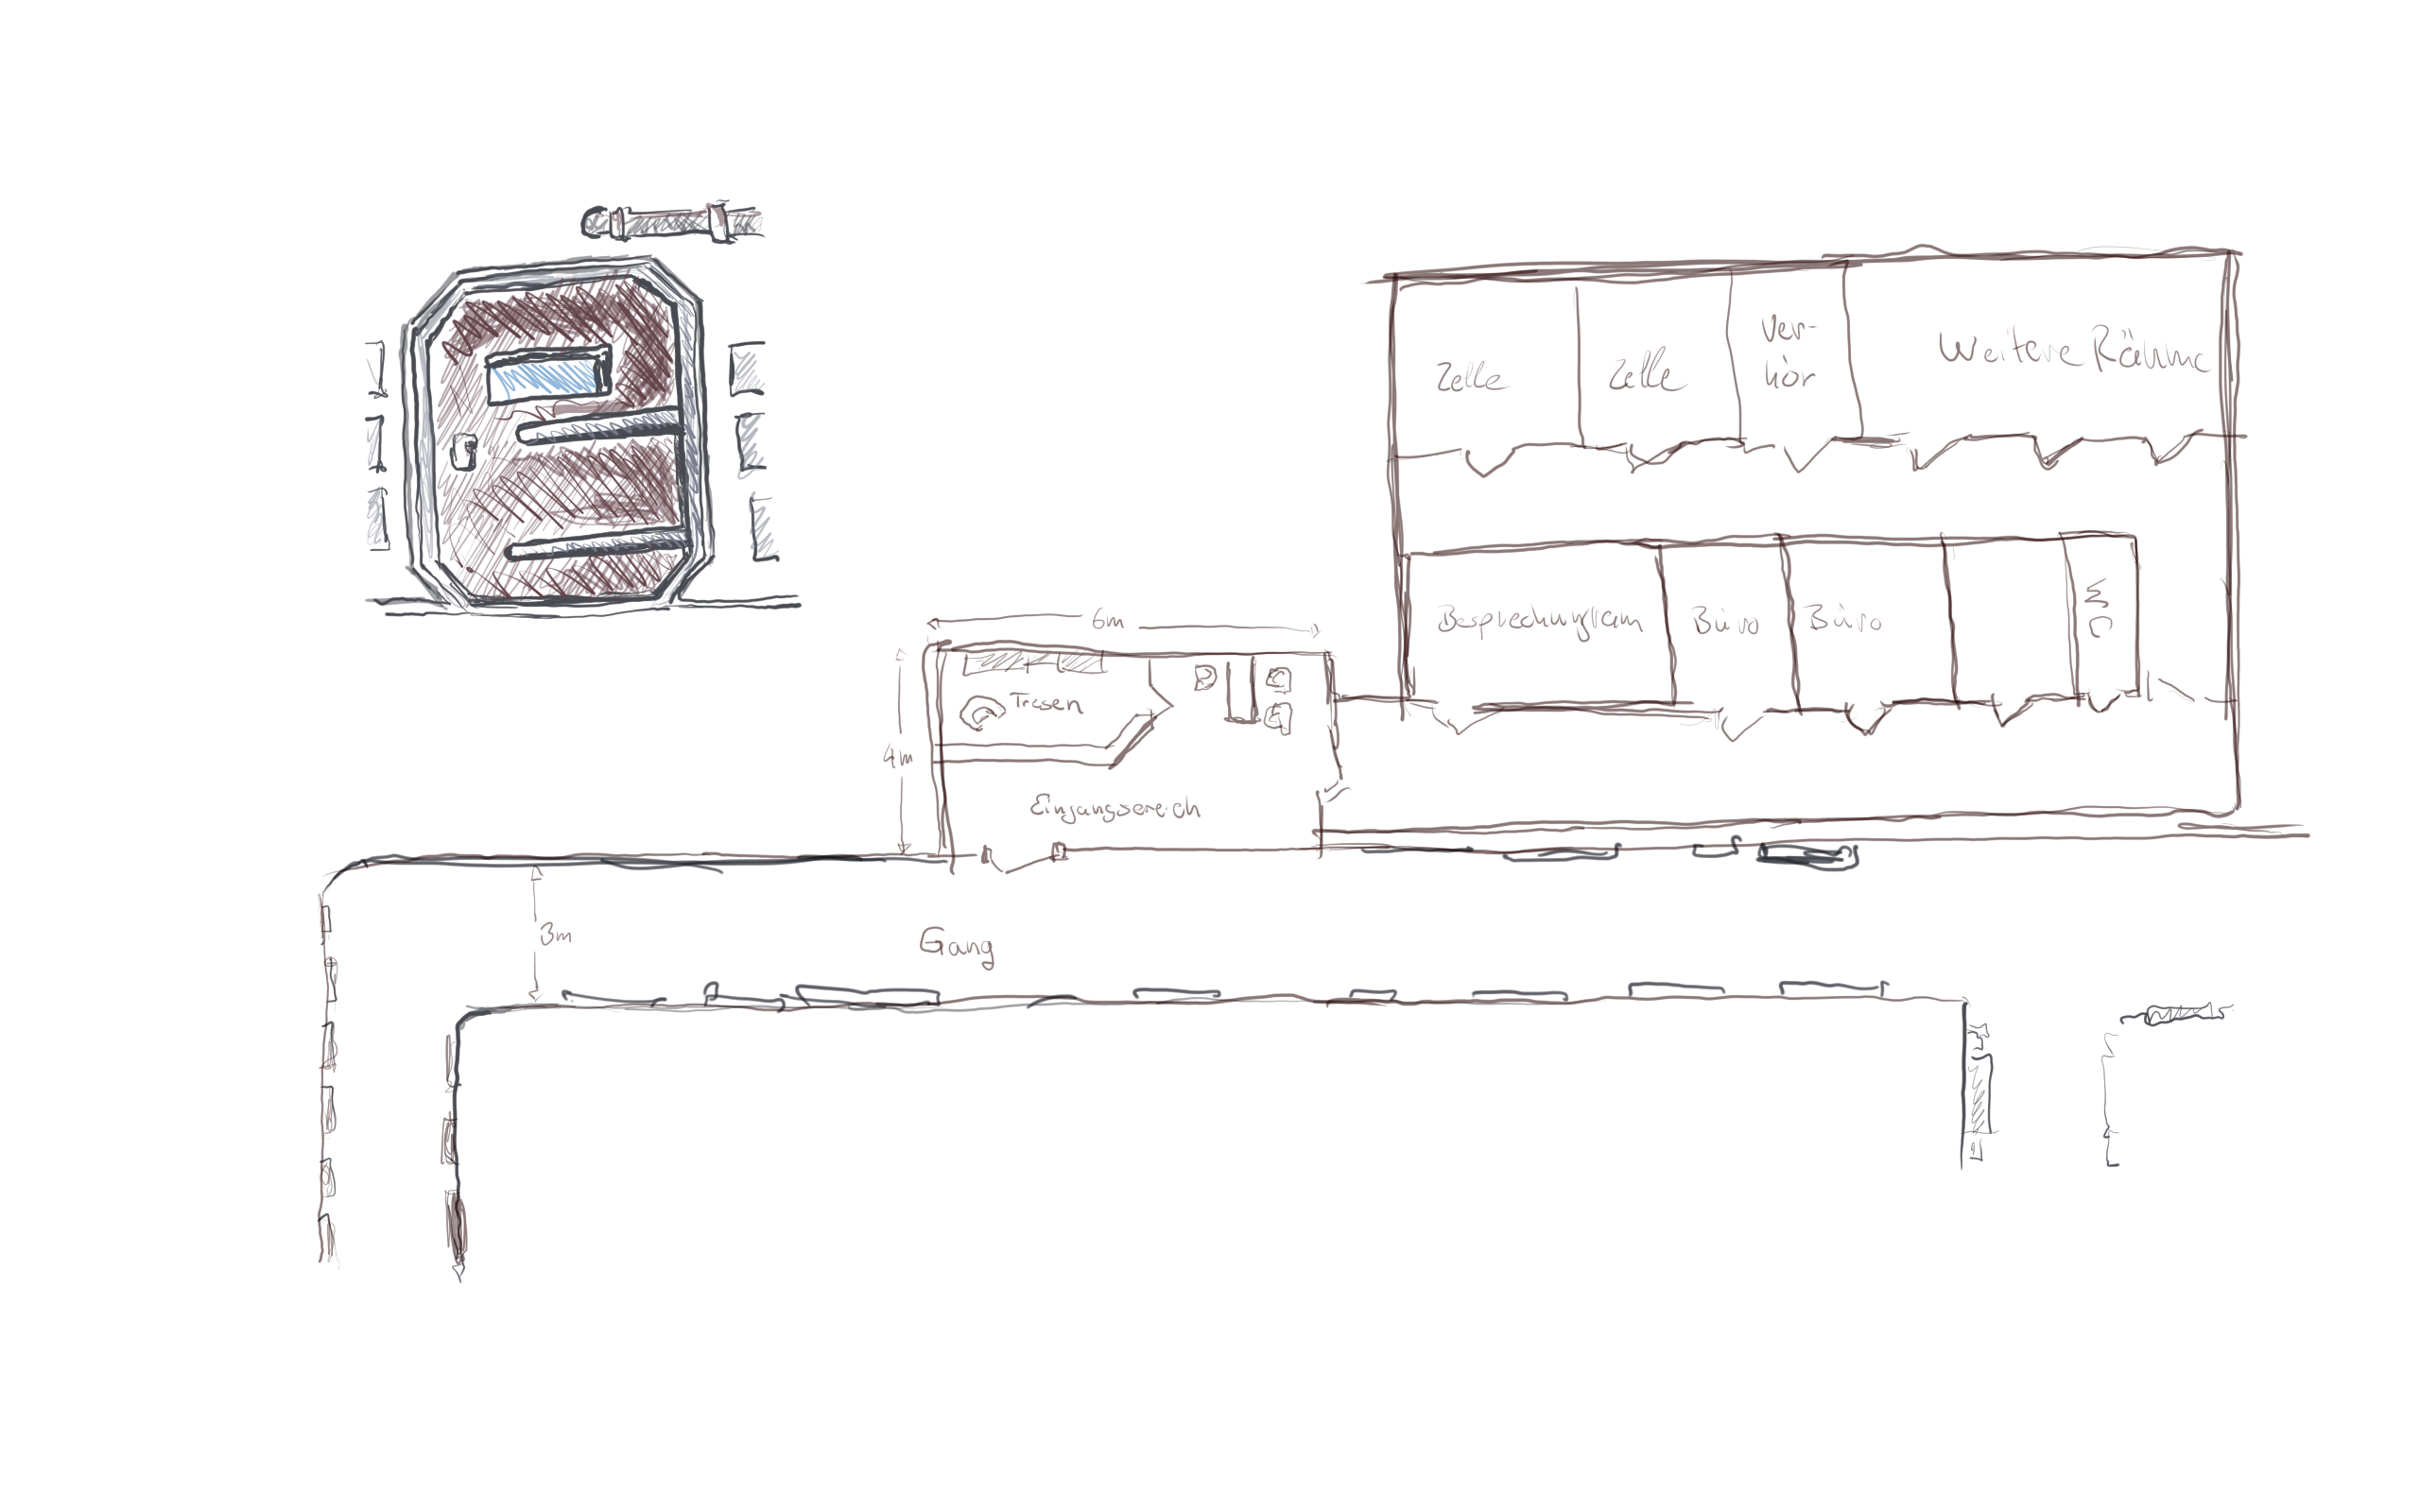
\includegraphics[width=0.9\linewidth]{./images/sicherheitdienst.png}
    \newline{}St"utzpunkt Sicherheitsdienst
	\label{fig:stuetzpunkt-sicherheitsdienst}
\end{figure*}

Zuvor: Wenn Handerson und Slingshot den Eingangsbereich des St"utzpunktes unter Kontrolle haben "offnen sie mit der Chipkarte von Karl Sandos oder Luke Lengdon die T"ur zu den hinteren R"aumlichkeiten, den Gef"angniszellen, dem Verh"orraum und anderen B"uros. Die Angreifer sperren die Charaktere und Karl Sandos in eine Zelle zusammen mit den Minenarbeitern und verlassen den St"utzpunkt mit Hanibal, einem der Charaktere und den beiden Frauen der Minenbesatzung als Geisel. Sie hinterlassen im hinteren Teil des St"utzpunkt einen St"orsender, der das ComNetz in der Umgebung des St"utzpunktes ausschaltet, und ein Funkger"at.  

St"urmen die Ermittler den Eingangsbereich des St"utzpunkts k"onnen sie den Eingangsbereich weiter untersuchen. Der Tresen kann mit einer Chipkarte von Grace Anders betreten werden. Hinter dem Tresen sind weitere Blutspuren zu entdecken. N"ahern sie sich der T"ure in die inneren Bereiche oder versuchen die Attent"ater direkt anzusprechen h"oren sie eine Stimme hinter der T"ure die droht die T"ure nicht zu "offnen sonst w"urden Geiseln sterben. Bei dem Sprecher handelt es sich um Slingshot der "uber Sprechfunk solange wie m"oglich versucht den Eindruck zu vermitteln die Entf"uhrer bef"andenden sich im St"utzpunkt. Kurz nachdem die Charaktere den St"utzpunkt betreten haben treffen  weitere Mitarbeiter vom Sicherheitsdienst in Begleitung von zwei Sanit"atern ein. Teil des Eingreiftruppe sind zwei Norms und ein Alpha. Sie tragen die Sicherheitswesten des Sicherheitsdienstes und jeweils einen Bolter. Die Sanit"ater sind Norms. Da es sich bei Hellgate um einen Cynarian St"utzpunkt handelt sind keine Omegas, Streitkr"afte des Protektorats, auf Hellgate verf"ugbar. Angef"uhrt wird der Trupp durch \emph{Luke Dexter} der sich direkt "uber den Verfall in Kenntnisse setzen l"asst. W"ahrenddessen l"asst er durch seine Leute unter Unterst"utzung der Ermittler und Grace den Eingangbereich und die G"ange absichern. 

Im Zellentrackt: Im Zellentrackt ist die andere Gruppe von Charakteren zusammen mit den Minenarbeitern eingesprerrt. Es fehlen Personen aus beiden Lagern. Auch ist nicht bekannt wo sich die Entf"uhrer aufhalten. Die Charaktere h"atten jetzt Zeit zu versuchen sich zu befreien oder sich bemerkbar zu machen. Die Zellen sind auf Randalierer und f"ur Aufst"andler gedacht dementsprechend nicht so gut gesichert wie eine Gef"angniszelle. Auch wenn das ComNetz lahmgelegt ist die T"ur nicht ohne passendes Werkzeug zu knacken. Ben"otigt w"aren ein Magschlossknacker oder Werkzeug zum kurzschlie\3en der Hydraulik. M"oglicherweise k"onnen hier aber Gegenst"ande aus dem Raum oder den 
Taschen der Minenarbeiter zweckentfremdet werden. Auch ein Lichtschacht w"are eine M"oglichkeit zumindest Kontakt nach au\3en aufzunehmen. 
Der Spielleiter sollte je nach Spielflu\3 entscheiden wie viel Zeit an dieser Stelle zur Verf"ugung steht.

Auf der Flucht: W"ahrend der Vorkommnisse im St"utzpunkt sind die Entf"uhrer zusammen mit ihren Geiseln auf dem Weg zu ihrem Shuttle um Valhalla zu verlassen. Kurz nach dem Verlassen des St"utzpunktes haben die Angreifer ihre Kampfausr"ustung gegen schu\3sichere Westen und einfache Bolter getauscht um nicht so leicht aufzufallen. Slingshot, Smith Handerson und Hanibal sind jeweils mit einer Schu\3waffe bewaffnet und treiben die Geiseln vor sich her. Um die PAN Systeme der Geiseln zu st"oren nutzen die Geiselnehmer ein St"orsender mit kurzem Radius.

Verhandlung mit den Entf"uhrern: Wurde der Eingangsbereich des St"utzpunkts abgesichert k"onnen die Charaktere zusammen mit Luke Dexter in Verhandlung mit den Entf"uhrern treten oder die hinteren R"aume des St"utzpunktes st"urmen. Fordern die Charaktere nach einem Lebenszeichen ihrer Freunde kann Slingshot den entf"uhrten Charakter bitten ein kurzes Wort von sich zu geben bei dem dieser versuchen kann eine Botschaft zu "ubermitteln.

\begin{remarks}
	Die Geiselszene ist auf einen schnellen Szenenwechsel zwischen den Charakteren im St"utzpunkt und den Charakteren die anderweitig Nachforschungen betreiben ausgelegt. Die Szenenwechsel sollten immer so erfolgen dass die \emph{Spieler} nur die wesentlichen Information erhalten die auch ihren Charakteren zur Verf"ugung stehen. D.h.~vor allem mu\3 ein Szenenwechsel erfolgen bevor die Geiselnehmer den St"utzpunkt wieder verlassen damit keiner der Spieler zun"achst erf"ahrt welche weiteren Schritte die Geiselnehmer einleiten.

	Slingshot steht mit Artisan dem Stellvertreter des Protektors und weiterem Attent"ater in Kontakt ohne seine Identit"at zu kennen. Im Auftrag der USI Agenten wird er durch Handerson auf Armageddon eingesammelt und fliegt mit ihm nach Hellgate bevor die Charaktere dort ankommen. Er kann dadurch verfolgen wie Hanibal zusammen mit den anderen Minenarbeitern zum St"utzpunkt der Sicherheitsmannschaft gebracht wird.

	Der erste Angriff sollte so ausgelegt werden, dass die Angreifer die Oberhand behalten aber keiner der Charaktere get"otet wird.
\end{remarks}


\newsection{Showdown auf Hellgate}

Die Entf"uhrer haben ihr Shuttle auf der Au\3enseite von Adrastea bei einer Wartungsschleu\3e nahe dem Raumhafen verankert. Nachdem die Charaktere im St"utzpunkt herausgefunden haben, dass sich die Entf"uhrer nicht mehr dort befinden gibt es mehrere M"oglichkeiten die Entf"uhrer aufzusp"uren. Am Erfolgsversprechenden w"are es die nach wie vor auftretenden St"orungen im ComNetz der Station zu verfolgen. F"ur die Navigation im St"utzpunkt m"ussen die Entf"uhrer kurzzeitig den St"orsender deaktivieren. Das gibt den Geiseln die M"oglichkeit eine kurze Nachricht zu "ubermitteln.

Folgende Szenarien die Entf"uhrer zu stellen sind denkbar:

\begin{description}
	\item [Lagerkomplex] Im Lagerkomplex des Raumhafens g"abe es die M"oglichkeit einen Hinterhalt zu legen und die Entf"uhrer zu 		
		"uberraschen.
	\item [Wartungsschleuse] Die Attent"ater und ihre Geiseln haben Hellgate verlassen und dabei ihr Shuttle zu betreten.
	\item [Shuttleverfolgung] Ist das Shuttle bereits gestartet bleibt den Charakteren nur das Shuttle zu verfolgen und zu entern um die 	
		Gefangenen zu befreien.
\end{description}


Wartungsschleuse: Hellgate besitzt neben dem Raumhafen eine Reihe von Ausg"angen die "uber Tunnel an die Oberfl"ache des Mondes erreichbar sind. Sie dienen als Flucht und Rettungstunnel oder geben Zugang zu verschiedenen Sensorplattformen zumeist in Richtung des Jupiter. Das Shuttle der Entf"uhrer hat auf einer Landeplattform mit seinen Andocklammern festgemacht. Der Zugangsbereich zum Landedeck umfasst zwei Luftschleu\3en: Eine als zu- und Ausgang f"ur Personen, eine zweite als Eingang f"ur Frachtcontainer. Eine Transportgondel f"ahrt "uber 500m zu einem gro\3en Zwischenlager. Ein Tender"ahnliches Schienenfahrzeug erlaubt es Material von einem angedockten Schiff zur Schleuse zu transportieren. Der Weg zum Landebereich ist "Uberdacht.  Die Schwerkraft auf Adrastea ist vernachl"assigbar. Es herrscht mehr oder weniger Schwerelosigkeit. Trotz Magnetstiefeln sollten sich Personen an Handl"aufen einhaken.

Shuttleverfolgung: Die Entf"uhrer versuchen in niedrigem Orbit zu fl"uchten um eine Verfolgung zu erschweren. In der N"ahe des Jupiter sind Sensoren nur eingeschr"ankt nutzbar. Dies wiederum erlaubt es Angreifern unerkannt von hinten im Schatten des Fusionstriebwerks anzugreifen. Die Geiseln sind im Shuttle im Laderaum eingesprerrt. F"ur ein Enterman"over ist die Dawn of Day am ehesten geeignet. Mit einem Dockingtunnel kann sie an das Shuttle der Entf"uhrer andocken. Die Schleuse in das Schiff kann entweder mit einem Magschlo\3knacker entriegelt oder aufgeschwei\3t werden. Torro Alvarez ist bereit mit seinen Valkyrien den Ermittlern Flankenschutz zu bieten und f"ur ein Ablenkungsman"over zu sorgen indem er mit den Entf"uhrern in Verhandlungen tritt. Einer Valkyrie bietet neben einem Piloten auch einer zweiten Person Platz.

Hanibal und Slingshot werden um jeden Preis versuchen ihrer Gefangennahme zu entgehen Der S"oldner hingegen ist nicht bereit bei dieser Mission zu sterben. Den Kampf mit Hanibal und Slingshot sollte

\begin{remarks}
	Bei den drei Optionen ist zu beachten, dass sie in Herausforderung und Zeitaufwand von oben nach unten gestaffelt sind. Zum Zeitpunkt der Entf"uhrung ist der Plot ca.~zu einem Drittel gespielt. Der Spielleiter sollte je nach angepeilter Spieldauer sich f"ur eine der Optionen entscheiden.

	Bei der "Uberw"altigung der Entf"uhrer sollte der Spielleiter anpeilen dass sowohl Hanibal als auch Slingshot get"otet oder so stark verletzt werden dass sie nicht mehr verh"ort werden k"onnen. Wurde Hanibal keinem Gehirnscan unterzogen sollte nachfolgend einem Psynchonauten ein Gehirnscan erm"oglicht werden.
\end{remarks}

%% Copyright 2019 Bernd Haberstumpf
%% License: CC BY-NC
% !TeX spellcheck = de_DE
\newsection{Hellgate Debriefing} 

Kurz nach dem Sieg "uber die Entf"uhrer, nachdem verletzte Charaktere wieder weitestgehend handlungsf"ahig sind, laden Vandermool, Avenger und Blackheart die Ermittler zu einem geheimen virtuellen Treffen in einem hermetisch abgeschirmten Raum der Hellgate-Station ein. Die drei sind bei diesem Treffen nicht pers"onlich anwesend, sondern werden holografisch in den Raum projiziert. Das Ermittlerteam kann nochmals in allen Details "uber die Geschehnisse berichten.

Die Ereignisse auf Hellgate werden von Vandermool, Avenger und Blackheart als kritisch eingesch"atzt. Attent"ater aus den eigenen Reihen mit einem fremdgesteuerten Gehirn sind sowohl f"ur die Cynarian-Aktivit"aten auf dem Jupiter als auch f"ur das Protektorat eine ernsthafte Gefahr. Des Weiteren haben die Ereignisse ein bisher in diesem Ma\3e nicht vorhandenes Misstrauen zwischen Cynarian und dem Protektorat ausgel"ost. Avenger und vor allem Blackheart bef"urchten eine verdeckte Operation der Cynarian Corporation. Vandermool ist beunruhigt, dass die Geschehnisse genau diese Reaktion ausl"osen k"onnten. Beunruhigend ist, dass weder der Feind noch der Ursprung der Bedrohung bekannt sind. Das hei\3t, eine Form von Gegenwehr ist zum aktuellen Zeitpunkt nicht m"oglich.

Vandermool und Blackheart sticheln gegeneinander, weil Blackheart eine milit"arische Aktion bevorzugt. Avenger versucht zu vermitteln. Am Ende einigen sich die drei Parteien darauf, die neu gewonnenen Erkenntnisse geheim zu halten, um die Gegner nicht aufzuschrecken und den gegenw"artigen Wissensstand nicht offenlegen zu m"ussen. Der Punkt geht an Vandermool und Avenger. Die Ermittlungen unauff"allig weiterzuf"uhren wird nach hitziger Diskussion als sinnvollstes Vorgehen beschlossen. Neben dem vorrangigen Ziel, im Verborgenen Informationen zu sammeln, m"ochte man eine Panik unter den Bewohnern des jovianischen Systems vermeiden. Die Sicherheit des jovianischen Systems unterliegt somit nun der Ermittlergruppe. Weitere Nachforschungen m"ussen unter strengster Geheimhaltung fortgesetzt werden.

Die Entdeckung der Gehirnmanipulation deutet auf ver"anderte kybernetische Module hin, die auf Kallisto eingesetzt wurden. Aus diesem Grund werden die Charaktere angewiesen, dort ihre Nachforschungen fortzuf"uhren. Da in einem Monat eine wichtige Konferenz geplant ist, bleibt wenig Zeit, die Hintergr"unde der Attentate aufzukl"aren. Den Ermittlern wird deshalb eine Frist von drei Wochen gesetzt, ohne die Konferenz selbst zu erw"ahnen.

Veranlasst durch Vandermool werden die Leichen oder verletzten Attent"ater umgehend zur Nike Station transportiert, um dort n"aher untersucht werden zu k"onnen. Blackheart setzt durch, dass Mitglieder der Mutantennation den Untersuchungen beiwohnen. Sie entsendet zwei Omega-Soldaten mit den Namen \emph{Stomper} und \emph{Bullet} nach Nike.

\begin{remarks}
	Das Briefing auf Hellgate ist die erste und einzige Gelegenheit w"ahrend der Geschichte, bei der Vandermool, Avenger und Blackheart zusammen in Erscheinung treten.


	Das Gespr"ach zeigt das dominante Auftreten Vandermools und das aufbrausende Wesen Blackhearts. Neben der Offenlegung der politischen Verh"altnisse dient die Zusammenkunft im Wesentlichen dazu, die Spieler in Richtung Valhalla zu lenken und die Nachforschungen auf Hellgate zu beenden.

	Um die Entfernung von mehr als einer Million Kilometern zwischen den einzelnen Orten der Gespr"achspartner zu vermitteln, sollte der Spielleiter die "Ubertragungszeit von mehreren Sekunden in die Dialoge einstreuen.

	\underline{Die Konferenz:}

	In einem Monat nach den aktuellen Ereignissen wird eine Delegation aus dem \emph{Shigano-Kombinat}, der st"arksten wirtschaftlichen Einrichtung auf dem Mars, und der \emph{Europ"aischen F"oderation} erwartet.  Es handelt sich um eine 
	politisch-wirtschaftliche Konferenz beschrieben \cref{sec:conference}. F"ur das Protektorat sind Verb"undete au\3erhalb des jovianischen Systems f"ur die Zukunft wichtig. Auch will man die Lage der Mutanten nach den Auseinandersetzungen auf der Erde, die letztendlich zur Gr"undung des Protektorats gef"uhrt haben, verhandeln. Aufgrund der noch nicht gefestigten Position innerhalb der Fraktionen im Sternensystem w"ahren die von der USI geplanten Attentate bei so einer Konferenz ein herber R"uckschlag.
	
	Die Konferenz ist zum aktuellen Zeitpunkt noch als geheim eingestuft, weswegen sie den Ermittlern zerzeit noch vorenthalten wird.
\end{remarks}


% Kallisto
%% Copyright 2019 Bernd Haberstumpf
%% License: CC BY-NC
% !TeX spellcheck = de_DE
\newsection{Eintreffen auf Hellgate}

Der Flug von Armageddon dauert rund 10 ereignislose Tage  mit dem Shuttle Dawn of Day w"ahrenddessen sich die Gruppe mit dem Shuttle vertraut machen k"onnen. 

Die HeM05 ist beim Eintreffen der Ermittler an der gigantischen Schlepperinsel der Hellgate Station angedockt. Die Schlepperinsel ist ein 2 Kilometer langes und breites Raumfahrzeug das mit gewaltigen Schubd"usen bis in die "au\3eren Athmosph"arenregionen des Jupiter eintauchen kann um dort die HE-3 Mienen abzusetzen oder einzusammeln. Die Schlepperinstel schwebt beim Anflug auf Hellgate majest"atisch nahe dem Mond Adrastea "uber der gewaltigen Fl"ache des Jupiter. Kleinste Partikel bilden eine Schleier auf diesem niedrigen Orbit von 130'000 km "uber dem Planeten. Hellgate befindet sich bis auf den Anflugtunnel fast vollst"an dig im Inneren des Mondes. Die Station selbst besteht aus dem Raumhafen, technischen Anlagen, Lagerhallen und R"aumen und Wohnquartieren, Lokale, Bars und L"aden. Im Ganzen umfasst die Anlage ca.~30 km\textsuperscript{3}. Wie in alles neuen eilig aufgesetzen Einichtungen befinden sich viele Provisorien, nicht abgeschlossene G"ange und herumstehendes Material in der Station.

Beim Ansteuern des Anflugtunnels wird die Dawn of Day von der Flugkontrolle kontaktiert und nach einer Legitimation gefragt. Nach den ersten Formalit"aten wird das Shuttle "uber einen Leitstrahl in den Landungstunnel navigiert. Der Pilot in der Gruppe kann hierbei sein K"onnen unter Beweis\3 stellen. Dem Spielleiter bleibt "uberlassen wie weit er den Landeanflug ausschm"uckt. Beim Eintreffen im Raumhafen herrscht reger Betrieb, eine gro\3e F"ahre bringt gerade neue Minenarbeiter und holt Mitarbeiter die nach Kallisto abreisen m"ochten. Mehrere Shuttle werden gewartet. In einem separaten Bereich sind die Maschinen, 8 Valkyrien der J"agerstaffel untergebracht. 

Zum Zeitpunkt des Eintreffens der Gruppe ist die Mine HeM05 an der Schlepperinsel vert"aut und teilweise zerlegt. Die Minen HeM01 und HeM04 sind im Einsatz. Die Besatzung der zerst"orten HeM3 sind teils zur Erholung auf Kallisto und teils bereit wieder im Einsatz auf den anderen Minen.

Im Raumhafen angekommen werden die Charaktere bereits von \emph{Grace Anders} erwartet. Grace ist Teil des lokalen Sicherheitsdienstes der Cynarian Corporation. F"ur den Aufenthalt der Charaktere ist sie zur unterst"utzung der Ermittler von \emph{Henk Arongate} dem Chef des Sicherheitsdienstes abgestellt. Sie steht hiermit den Ermittlern w"ahrend ihres gesamten Aufenthalts treu zur Seite, kann Recherchen beauftragen, kennt die Station mit ihren verwirrenden G"angen und kann lokale Unterst"utzung anfordern. Beim Eintreffen wird sie die Ermittler aufkl"aren dass es sich um eine Minenkolonie handelt und dadurch die Gepflogenheiten etwas ruppiger seien k"onnen. Aus diesem Grunde tragen die Sicherheitskr"afte Schutzkleidung und eine Waffe. Desweiteren erfahren die Ermittler dass ihre Untersuchungen m"oglicherweise kritisch aufgenommen werden k"onnten da man meint die Vorkommnisse k"onnten auch lokal gekl"art werden.

\begin{remarks}
	Die Spieler k"onnen die ersten Information von Grace Anders dazu nutzen sich selbst passend auszur"usten. Kontaktieren die Ermittler Henk Arongate direkt wird er sie h"oflich begr"u\3en, verweist sie dann aber weiter an Grace. Grace Anders ist eine junge h"ubsche aber auch vor allem kompetente und loyale Unterst"utzerin. Sie dient dem Spielleiter den Spielern unter die Arme zu greifen sollten sie selbst nicht weiter kommen und bringt der"uber hinaus eine pers"onliche Note ins Spiel mit ein.
\end{remarks}

\pageimage{images/cmyk/hellgate_cmyk.jpg}
%% Copyright 2019 Bernd Haberstumpf
%% License: CC BY-NC
% !TeX spellcheck = de_DE
\newsection{Auf dem Garnisonsst"utzpunkt}
\bottomimage{images/armytank.png}

Ein erster Anlaufpunkt der Charaktere w"are vermutlich der Garnisonsst"utzpunkt des Protektorats, da dort die Cowboybrigade aufzufinden ist. Da Kallisto offiziell nicht dem Protektorat angeh"ort, unterh"alt das Milit"ar des Protektorats nur einen kleinen St"utzpunkt in Valhalla. Der St"utzpunkt beherbergt eine Kompanie von 40 Soldaten, gr"o\3tenteils Omega Krieger. Diesen angeschlossen sind Techniker und sonstiges Personal.

Der Oberbefehlshaber des St"utzpunktes ist der Omega \emph{Commander Lockhead}, der bereits "uber das Eintreffen der Ermittler informiert ist. Commander Lockhead ist ein in die Jahre gekommener Veteran mit unerwartet freundlichen Gem"ut. 

Nach der Untersuchung des Frachterungl"ucks auf Armageddon hat er die Cowboybrigade entweder auf Anweisung der Charaktere oder auf einen Befehl von Colonel Scholz hin inhaftieren lassen und h"alt sie seitdem in Untersuchungshaft. Der Commander ist "uber die Vorg"ange auf Hellgate informiert und bietet auch diesbez"uglich den Ermittlern seine Hilfe an. Er kann f"ur Untersuchungen im Umfeld des Raumhafens, der Garnison und der Oberstadt seinen Adjutanten \emph{Firedon}, einen jungen Omega-Soldaten, zur Verf"ugung stellen. 

Zu Fragen nach der Cowboybrigade kann Lockhead beitragen, dass als Vorbereitung f"ur den Einsatz neuer Drohnen und anderer technischer Ger"aten, die auch auf Armageddon zum Einsatz kamen, die ganze Cowboybrigade mit neuen Talentchips vor 2 Monaten in der Klinik \emph{Rondra Hospital} ausgestattet wurden. Die Kosten hat die Garnison "ubernommen. Die Cowboybrigade ist seit vier Monaten am Raumhafen f"ur Wartungsarbeiten an Schiffen und Ger"atschaften der Garnison zugeteilt. Auch nach ihrer Versetzung vom zivilen Teil des Raumhafens zur Garnison ist eine gewisse \emph{Sonja Frost} ihre personelle Vorgesetzte.

\begin{remarks}
	\underline{Gewonnene Information:}
	
	\begin{itemize}
		\item Die Cowboybrigade ist seit vier Monaten bei der Garnison im Raumhafen t"atig. 
		\item Vor 2 Monaten sind ihr neue Talentchips in der Rondra Klinik eingesetzt worden.
		\item Firedon wurde zur Unterst"utzung der Ermittler freigestellt.
		\item Der Kontakt zum Raumhafen ist Sonja Frost, der Chief Officer des Hangardecks.
	\end{itemize}

	F"ur Fahrten durch die Oberstadt bietet Firedon ein Milit"ar-Truck an.
	 
\end{remarks}

\newsection[Nachforschungen im Rondra Hospital]{Nachforschungen im Rondra\newline{}Hospital}

In Bezug auf das Rondra Hospital k"onnte der Verdacht aufkommen, dass dort die Manipulationen an den Gehirnen von Hannibal und Slingshot durchgef"uhrt wurden. Auf Dr"angen von Commander Lockhead w"are ein Termin mit dem Klinikleiter \emph{Prof.~Dr.~Henry Sanders} m"oglich. Die beiden Herren, so verschieden wie sie sind, kennen einander aus vergangenen Zeiten bei der Europ"aischen F"orderation.

Der Klinikleiter empf"angt die Charaktere in einem ger"aumigen B"uro. Sanders ist ein Norm im Alter von "uber 50 Jahren, mit gepflegtem Aussehen und grau meliertem Haar. Bei Fragen zur Cowboybrigade oder Hannibal, verweist er die Gruppe an \emph{Brenda Ben}, die er auch gleich bittet die Ermittler zu unterst"utzen. 

Brenda Ben ist eine sympathische und erfahrene "Arztin. Sie ist Mitglied des Leitungsteams der Klinik. Routiniert kann sie von 
\emph{Ben Reuthers} aus der Buchhaltung Unterlagen anfordern und die Ermittler im Fall der Cowboybrigade an den behandelnden Chirurgen \emph{Dr. Loyd Rothan} sowie die Physiotherapeuten \emph{Russel Spenser} und \emph{Phillip Klarson} weiterleiten. Hannibal ist in den Akten des Rondra Hospitals nicht verzeichnet. Brenda Ben hat jedoch nur begrenzt Zeit und verabschiedet sich nach dieser ersten Recherche, da sie zu einer Operation gerufen wird.

Dr. Loyd Rothan best"atigt das Einsetzen der Talentchips, bei allen Mitgliedern der Cowboybrigade, durchgef"uhrt zu haben. Nach den erfolgreichen Eingriffen trainierten die Physiotherapeuten die Wartungstechniker im Umgang mit ihrer neuen Cybertechnologie. Ben Reuthers best"atigt die Beauftragung der Operation durch Sonja Frost und die Zahlungsabwicklung durch die Garnison.

Die Informationen aus der Klinik entsprechen denen von Commander Lockhead.

\begin{remarks}
	\underline{Gewonnene Information:}
	
	\begin{itemize}
		\item Neue Kontakte: Prof.~Dr.~Henry Sanders, Brenda Ben, Ben Reuthers, Dr. Loyd Rothan, Russel Spenser und Phillip Klarson.
		\item Eingriff bei der Cowboybrigade im Rondra Hospital ist unauff"allig. Keine besonderen Vorkommnisse.
		\item Hannibal wurde nicht im Rondra Hospital operiert.
		\item Die Aussagen am Hospital decken sich mit den Aussagen von Commander Lockhead.
	\end{itemize}

	\underline{Prof.~Dr.~Sanders:}

	Wie sich sp"ater herausstellen wird, ist Sanders viel tiefer in die Vorkommnisse mit den implantierten KIs involviert, als sich zum aktuellen Zeitpunkt erahnen l"asst. Bei der Cowboybrigade wurden aber in seiner Klinik nur die beauftragten Talentchips installiert. Der Professor kann deshalb die Ermittler guten Gewissens an seine Mitarbeiter verweisen.
\end{remarks}

\newsection{Cowboybrigade Voruntersuchung}

Gehen die Charaktere davon aus, dass weitere Mitglieder der Cowboybrigade ebenfalls einer Gehirnmanipulation unterzogen wurden, k"onnen sie Firedon beauftragen einen der vier in einer Klinik untersuchen, zu lassen. Das Rondra Hospital f"uhrt als gr"o\3tes Hospital in Valhalla alle medizinischen Eingriffe f"ur den Garnisonsst"utzpunkt durch. Vertrauen die Charaktere dem Rondra Hospital nicht, schl"agt Firedon die davon unabh"angige \emph{Alexandr Clinic} vor. 

Da nicht bekannt ist, ob sich ein weiteres Mitglied der Cowboybrigade als Attent"ater entpuppen k"onnte, sollten die Charaktere die Verd"achtigen zu diesem Zeitpunkt nicht in die Vorg"ange auf Hellgate oder Attentatsverd"achtigungen einweihen.

Werden die Untersuchungen in der Alexandr Clinic durchgef"uhrt, zeigt sich der leitende Arzt Dr.~Spinner zwar zun"achst erstaunt, warum man sich an seine Klinik und nicht an das Rondra Hospital wendet, ist aber bereit eine Untersuchung durchzuf"uhren. 

Bei den nicht invasiven Untersuchungen durch eine Klinik lassen sich keine Manipulationen feststellen. Die implantierten technischen Einheiten wirken nach Aussage der "Arzte unauff"allig. Die Gehirnwellen weisen ebenfalls keine Anomalien auf. Wenn die Charaktere allerdings noch keine n"aheren Informationen von der Nike Station erhalten haben, ist auch nicht klar auf was ein Arzt achten sollte. 

Selbst mit den weiter unten beschriebenen Informationen aus der Nike Station werden bei der Untersuchung keine Auff"alligkeiten festgestellt. Der Rest der Cowboybrigade ist ebenfalls sauber.

\begin{remarks}
	\underline{Gewonnene Information:}
	
	Eine Untersuchung des Gehirns der Mitglieder der Cowboybrigade zeigt keine auff"alligen Anomalien.
\end{remarks}

\newsection{R"uckmeldung von Nike}\anchor{sec:nanobots}

Zwei Tage nach ihrer Ankunft werden die Ermittler von Dr. ~\pinyin{Wang2} \pinyin{Chen2} kontaktiert.  Er f"uhrte die Untersuchungen an den K"orpern von Slingshot und Hannibal auf der Nike Station durch.

Bei den get"oteten Attent"atern konnte Dr. \pinyin{Wang2} \pinyin{Chen2} inaktive Nanobots entdecken. Diese Nanobots haben sich umfassend mit den Synapsen im gesamten Gehirn verbunden. Wurden einer der Attent"ater oder beide nicht get"otet, konnten elektrische Impulse gemessen werden, die weder dem Gehirn selbst noch dem Kontrollmodul zuordenbar waren. Die genaue Funktion der Nanobots konnte noch nicht entschl"usselt werden, aber es wird von einem hochkomplexen verteilten System ausgegangen.

Eine weitere Auff"alligkeit sind die in den K"opfen implantierten Kontrollmodule. Es handelt sich um Modelle neuester Generation, hergestellt von \emph{Kasai Cyber Genetics}, die "uber einen modifizierten Nanitenspender verf"ugen. Die Nanitenspender dienten vermutlich der Aussch"uttung der Nanobots. Kasai Cyber Genetics ist ein Technologieunternehmen mit Sitz auf dem Mars, das dem Shigano-Kombinat angeh"ort. Ihre Kontrollmodule sind beliebt, aber vergleichsweise kostspielig.
\vfill

\begin{remarks}
	\underline{Gewonnene Information:}
	
	\begin{itemize}
		\item ie beiden Attent"ater haben ein hochmodernes Kontrollmodul von Kasai Cyber Genetics, das einen modifizierten Nanitenspender in 
			ihren K"opfen enth"alt.
		\item Die Bewusstseinsver"anderung der Attent"ater wurde durch Nanobots im Gehirn ausgel"ost.
	\end{itemize}
	
	\underline{Nanobots:}

	Bei den Nanobots handelt es sich um die eigentliche KI, die mithilfe des Kontrollmoduls in das Gehirn gelangt. Das Kontrollmodul dient den KIs zur Kontaktaufnahme mit Agenten der USI, um von diesen Befehle zu erhalten. Bei jedem Kontakt mit einem ComNetz k"onnen die USI-Agenten der KI Anweisungen erteilen.

	\underline{Kontrollmodul:}

	Das implantierte Kontrollmodul ist ein leicht angepasstes Standardmodell. Kasai Cyber Genetics ist nicht in die Attentate verwickelt.
\end{remarks}

\newsection{Sonja Frost}

Eine weitere Anlaufstelle im Zentrum von Valhalla ist Sonja Frost. Sie ist die Chief Officer des Hangar-Decks des Raumhafens. Sonja Frost ist dementsprechend schwer zu erreichen. Ein Anruf durch den St"utzpunkt ist notwendig, um "uberhaupt einen Termin zu vereinbaren.

Sonja ist in ihrem B"uro neben dem Hangar anzutreffen. Das B"uro ist mit technischen Ger"aten, Holoprojektoren und Tafeln vollgestellt. Es herrscht ein reges Rein und Raus, und Sonja verteilt durchgehend Anweisungen.

Von Sonja erfahren die Ermittler, dass die Cowboybrigade vor ca.~1\half~Jahren vom Asteroideng"urtel zwischen Mars und Jupiter in das Jovianische System wechselte und dort am Raumhafen untergekommen ist. Vor vier Monaten wurden sie dann an das Milit"ar "uberwiesen. Der medizinische Eingriff bei der Cowboybrigade wurde in Abstimmung mit Commander Lockhead beschlossen und erwartungsgem"a\3 durchgef"uhrt und bezahlt.

Sonja Frost berichtet, dass die Mitglieder der Cowboybrigade am Raumhafen unter dem Pseudonym "`die glorreichen F"unf"' bekannt sind. Aufgrund ihrer heiteren, skurrilen Art, aber auch wegen ihrer Zuverl"assigkeit, sind sie im Hangar-Deck beliebt und wertgesch"atzt. Den Spitznamen Cowboybrigade erhielten sie erst durch die Besch"aftigung in der Garnison, als sie begannen, gegen"uber Stetson zu salutieren. Nach dem Einsetzen der Talentchips im Rondra Hospital kehrten die F"unf nach zwei Wochen wieder zum Dienst zur"uck. Slingshot meldete sich allerdings ein paar Tage sp"ater krank und kehrte erst nach weiteren zwei Wochen, kurz vor der "Uberstellung nach Armageddon, zur"uck. N"aheres kann sie dazu auch nicht beitragen.

Bez"uglich Hannibal muss sie in ihrem Terminal nachforschen. V"ollig ungewohnt benutzt sie daf"ur ein Ger"at ohne neuronales Interface. \say{Abgeschottetes System, aus Sicherheitsgr"unden}, sagt sie, wenn man sie danach fragt und grinst. Schnell wird sie f"undig. Hannibal hat vor neun Monaten seine Arbeit am Raumhafen als Softwaretechniker begonnen. Vor zwei Monaten wechselte er seinen Arbeitsplatz und bekam eine Anstellung bei Cynarian als Sicherheitstechniker auf der Minenkolonie Hellgate. Einen Monat vor seiner K"undigung hatte er sich f"ur 14 Tage krankgemeldet.

Bevor die Charaktere das B"uro verlassen, f"allt ihr noch ein, dass sich nach der Landung der Dawn of Day zwei Herren in Anz"ugen nach den Ank"ommlingen erkundigt haben. Einer der beiden war gro\3, hatte eine T"ursteherstatur und einen sehr gepflegten blonden B"urstenhaarschnitt. Der andere war unauff"allig und hatte nicht gesprochen. Informationen "uber die Ermittler konnten den beiden nicht gegeben werden (O-Ton: "`K"onnte ja jeder kommen"'). Aufzeichnungen von den beiden sind ihr nicht bekannt.

\begin{remarks}
	\underline{Gewonnene Information:}
	
	\begin{description}
		\item[Cowboybrigade] Die Cowboybrigade alias "`die glorreichen F"unf"' ist seit 1\half Jahren im jovianischen System und seitdem am 
			Raumhafen t"atig. Seit 4 Monaten sind sie bei der Garnison besch"aftigt. Vor zwei Monaten wurden ihnen Talentchips eingesetzt. Slingshot meldete sich danach insgesamt f"ur zwei Wochen krank.
		\item[USI-Agenten] Zwei Anzugtr"ager haben sich nach der Dawn of Day erkundigt. Bei den beiden handelt es sich um die USI-Agenten  
			\emph{Smith-Singer} und \emph{Frederic Johnson}. Smith-Singer ist der f"uhrende Drahtzieher hinter der Operation P9 und den Attentaten im jovianischen System. Frederic Johnson ist ein Psychonaut, der Smith-Singer unterst"utzt. Weiteres findet sich im \cref{sec:usiagents}.
	\end{description}
\end{remarks}


\newsection{Die Cowboybrigade im Verh"or}

Die Ermittler k"onnen Firedon beauftragen, die inhaftierte Cowboybrigade in einem Verh"orraum vorzuf"uhren. Stetson l"ummelt beim Eintreten der Charaktere mit einem Zahnstocher im Mund und einem verbeulten Cowboyhut auf dem Kopf in seinem Sitz. Beim "Offnen der T"ur setzt er sich abrupt aufrecht. Quicksilver Rod mischt nerv"os, aber virtuos ein Deck Spielkarten. Joe Rider sitzt finster dreinblickend und eingesunken auf seinem Stuhl. Tom Gunslinger wendet den Blick erwartungsvoll in Richtung der Eintretenden. Werden die Vier zusammen befragt, wendet sich Stetson als Erster an die Charaktere und fragt, was ihnen vorgeworfen wird, was mit Slingshot los ist und wann sie wieder entlassen werden. Sie gehen nach wie vor davon aus, dass es sich beim Frachterungl"uck auf Armageddon um einen Unfall gehandelt hat.

Konfrontieren die Ermittler die Truppe teilweise oder vollst"andig mit den wahren Gegebenheiten auf Armageddon oder Hellgate, beteuert Stetson entgeistert ihre Unschuld. Er versichert, nach einem Blick zu den anderen, Auskunft zu allen Fragen zu geben. Er beteuert, dass seine Freunde und er sicher nichts zu verbergen h"atten.

Quicksilver Rod blickt bei einer Befragung immer wieder zu Stetson. Seine Finger scheinen dabei ein Eigenleben zu f"uhren. Ein Kartentrick folgt dem anderen, ohne das Rod Notiz davon nimmt. Bei Joe Rider vergeht nach jeder Frage erst eine halbe Minute bevor er antwortet. Die Antworten beschr"anken sich dann nur auf das Gefragte und enthalten nicht ein unn"otiges Wort. Tom Gunslinger ist das genaue Gegenteil. Gef"ahrlich wild gestikulierend, mit einem Trinkbecher in der Hand, schie\3en Worte aus seinem Mund. St"andig schweift er von dem aktuellen Thema ab.

Auf eine psychonautische Untersuchung reagiert die Gruppe leicht panisch. Keiner hat eine Vorstellung was auf sie zukommt k"onnte. Die Untersuchung lassen sie dann aber "uber sich ohne Gegenwehr ergehen. Ein Gehirnscan best"atigt, dass ihre Gehirne sauber sind und dass ihre Aussagen ihrem Wissensstand entsprechen. 

Angesprochen auf die Eingriffe in der Rondra Klinik schildern sie, dass sie in der Klinik neue Talentchips mit anschlie\3endem Training erhalten haben. Eine Frage, ob es bei Slingshot Komplikation gegeben h"atte, wird verneint. Allerdings erfahren die Ermittler, dass Slingshot im Gegensatz zu den anderen kein ausgebildeter Shuttle- und Drohnenpilot ist, sondern nur ein hervorragender Schiffstechniker. Slingshot hatte schon immer davon getr"aumt auch eine Flugausbildung zu erhalten. Offensichtlich hat er sich nach dem Aufenthalt im Rondra Hospital selbst auf die Suche nach einer entsprechenden Kontrolleinheit gemacht. Vor der Versetzung nach Armageddon wurde er dann f"undig. 
Ein erweitertes Kontrollmodul erlaubte es ihm Drohnen und Shuttles fernzusteuern. Wie er die daf"ur aufkommenden Gelder aufbringen konnte, wollte er den anderen nicht verraten. Ebenso wenig legte er offen, wo er den Eingriff hatte durchf"uhren lassen und wo er sich danach aufgehalten hat. 

Ein paar Tage nach der Entlassung aus dem Rondra Hospital hatte er angefangen die Freizeit oft alleine zu verbringen. "Uber den Barmann und Besitzer des Batcave konnten seine Freunde in Erfahrung bringen, dass er wohl eine h"ubsche Frau kennengelernt hatte. Darauf angesprochen tat er allerdings immer betont geheimnisvoll. Weitere Informationen sind von der Cowboybrigade nicht in Erfahrung zu bringen.

\begin{remarks}
	\underline{Gewonnene Information:}

	\begin{itemize}
		\item Slingshot hat sich eine Flugsteuerung implantieren lassen.
		\item Die Finanzierung des neuen Systems ist unbekannt.
		\item Slingshot hat eine Frau kennengelernt.
	\end{itemize}

	\underline{Carina:}
	
	Bei der geheimnisvollen Frau handelt es sich hierbei um Carina alias Fleur Soleil, auf die die Charaktere sp"ater in einem Club treffen werden. Die Identit"at der Freundin ist weder der Cowboybrigade noch dem Barmann im Batcave bekannt. Cariana ist im \cref{sec:carina} beschrieben.
\end{remarks}

\pageimage{images/cowboybrigade_cut.jpg}

%% Copyright 2019 Bernd Haberstumpf
%% License: CC BY-NC
% !TeX spellcheck = de_DE
\newsection{Zwischenfall auf Fenris (optional)}
% Gestrichehn da: Derzeit gibt es kein gutes Konzept bei dem Tiger nicht im Rondra Hospital operiert wurde aufmerksam
% ohne auf das Rondra Hospital zu machen.

Der Zwischenfall auf Fenris kann genutzt werden, wenn die Charaktere auf Hellgate nicht mit den KIs in den K"opfen der beiden Attent"ater in Kontakt kommen konnten. Der Vorfall hilft auch, ein aggressives Vorgehen von Blackheart im sp"ateren Spielverlauf verst"andlich zu machen. Er ist eine gute M"oglichkeit, die kosmonautischen F"ahigkeiten der Charaktere zum Einsatz zu bringen. Auf der anderen Seite verl"angert der Zwischenfall den Spielablauf signifikant, ohne zwingende Relevanz f"ur die Geschichte zu haben. Er ist deshalb als optional gekennzeichnet.

Beim Anflug auf Kallisto werden die Charaktere vom Kommandanten, Lord Commander Grendel, der Fenris-Station kontaktiert. Auf der Raumbasis konnte ein Attent"ater dingfest gemacht werden, der die Computersysteme der Station zu manipulieren versuchte. Beim Attent"ater handelt es sich um den Omega Commander Tiger. Commander Tiger beteuert, von dem Attentat nichts zu wissen, obwohl er sich seiner Festnahme widersetzte und einen Kameraden schwer verletzt hat. Die Ermittler werden gebeten, sich schnellstm"oglich auf der Fenris-Station einzufinden, um dem Verh"or beizuwohnen.

Beim Landeanflug auf die Fenris-Station kommt es zu einem unerwarteten Zwischenfall. Die Verteidigungsanlagen der Station nehmen das Shuttle der Ermittler unter Beschuss. Es kommt zu einem Druckverlust im Schiff, da Geschosse die Bordwand durchschlagen. Dar"uber hinaus kommt es zu einer Fehlfunktion des Zentralcomputers, was zu einer Notabschaltung des Fusionstriebwerks f"uhrt. Was genau passiert ist, erfahren die Passagiere zu diesem Zeitpunkt nicht. Das Schiff wird ordentlich durchgesch"uttelt, und die Passagiere werden unsanft aus der virtuellen Realit"at des Bordsystems gerissen. Notbeleuchtung und der Schiffsalarm weisen unmissverst"andlich auf den Ernst der Lage hin. Alle Passagiere tragen gl"ucklicherweise einen Druckanzug, um die Kr"afte bei Abflug und Anflug zu kompensieren, m"ussen aber noch die Atemmaske anlegen, die jeweils in einem Fach der Beschleunigungsliege bereitliegt. Nach dem Abschalten des Fusionstriebwerks tritt im Shuttle sofort Schwerelosigkeit ein. Bei einem Abstand von rund 1200 Kilometern rast das Shuttle nun mit 300 m/s auf die Fenris-Station zu.

Um das Haupttriebwerk erneut zu starten und die Steuerd"usen zu aktivieren, muss als Erstes der Zentralcomputer neu gestartet werden. Der Bordcomputer l"ost Kollisionsalarm aus. Mittels Man"ovrierd"usen muss die Flugbahn korrigiert werden, um an der Station vorbeizufliegen, doch die Steuerung kann die D"usen nicht ausrichten. Nur durch einen Au\3eneinsatz k"onnen die D"usen in Position gebracht werden.

W"ahrend ein oder zwei Ermittler die D"use manuell ausrichten, kann anderer die Funkanlage, die ebenfalls ausgefallen ist, wieder in Betrieb nehmen. Die Anlage muss auf die Notantenne umgeschaltet werden, da die Hauptantenne beim Angriff besch"adigt wurde. Ist die Funkanlage wieder verf"ugbar, kann ein Notruf abgesetzt werden, der von der Flugleitung der Fenris-Station beantwortet wird. Mit geknickter Stimme fragt der Flugleitstand nach der Situation auf der Dawn of Day und meldet, dass die Verteidigung der Station aufgrund einer noch nicht gekl"arten Fehlfunktion das Shuttle unter Beschuss genommen hat. Die Station entsendet daraufhin ein Rettungsshuttle, um die Dawn of Day zur Fenris-Station zu schleppen.

Lord Commander Grendel, in Begleitung von zwei weiteren Omega-Soldaten, nimmt die Ermittler pers"onlich in Empfang. Er erkl"art den Besuchern, dass vermutet wird, dass der Angriff auf das Shuttle mit dem Sabotageakt in Zusammenhang steht. Die Verteidigungsanlage ist derzeit komplett deaktiviert, heruntergefahren und vom Rest der Stationssysteme getrennt. Leider m"ussen Computerspezialisten, die dem Problem Herr werden k"onnen, erst angefordert und eingeflogen werden. Lord Marshal Blackheart ist bereits "uber die Vorkommnisse auf der Station informiert und hat angek"undigt, sich selbst vor Ort ein Bild machen zu wollen.

Laut Commander Grendel wurde Tiger "uberrascht, w"ahrend er sich im zentralen Computerkabinett an den Speicherb"anken zu schaffen machte. Als Nicht-Techniker h"atte er zu diesem Bereich keinen Zugriff gehabt und sollte eigentlich auch keine Expertise f"ur die Rechenanlage besitzen. Bei seiner Entdeckung griff er sofort zu seiner Bolzenpistole und feuerte mehrere Sch"usse auf den Sergeant der Patrouille ab, die ihn entdeckt hatte. Der Sergeant ging zu Boden. Sein Begleiter konnte Tiger "uberw"altigen und Hilfe anfordern. Bei der Erstbefragung beteuerte der Gefangene, sich in keinster Weise an die Vorg"ange erinnern zu k"onnen.

Commander Tiger ist in einer Arrestzelle zum Verh"or festgesetzt worden und wird dort von zwei Soldaten bewacht. Der Gefangene sitzt in einem durch Gitter abgesperrten Teil der Zelle. Im Besucherteil halten zwei bewaffnete Omega-Soldaten Wache. Der Attent"ater wirkt beim Eintreffen der Ermittler stark angespannt, bei\3t die Z"ahne zusammen und antwortet auf keine Fragen. Lord Commander Grendel erw"agt, Tiger durch Wahrheitsdrogen gespr"achig zu machen, will daf"ur aber erst die Ankunft von Blackheart abwarten. Bestehen die Ermittler darauf, einen Gehirnscan durchzuf"uhren, wird ihnen diese Bitte widerwillig gew"ahrt. Der Psychonaut des Teams muss daf"ur den abgesperrten Teil der Zelle betreten. Commander Tiger ist mit Hand- und Fu\3fesseln auf einem Stuhl fixiert. Betritt der Psychonaut den Gefangenenteil, wird Tiger pl"otzlich vollkommen ruhig und bekommt einen glasigen Blick. Kurz darauf l"osen sich die elektronisch verriegelten Fesseln, und er st"urzt sich auf den Ermittler. Die Wachen ziehen beide ihre vollautomatischen Bolzenpistolen und werden den Gefangenen niederschie\3en, sofern niemand eingreift und sie ein freies Schussfeld haben.

Kann der Gefangene lebendig "uberw"altigt werden, kann der Psychonaut zur Tat schreiten. Zum Attentat finden sich keine Erinnerungen, allerdings findet der Psychonaut seltsam artifiziell wirkende Gedankeng"ange mit Matrizen aus Entscheidungsb"aumen. Nach diesen ersten Erkenntnissen wird der Psychonaut mental angegriffen. Wie bei den beiden Attent"atern auf Hellgate wurde auch Tiger eine KI in das Gehirn eingesetzt. Ein "Uberwinden der KI f"uhrt unweigerlich zum Gehirntod des Commanders. Den letzten Gedanken, den der Psychonaut aufschnappt, ist \say{Rette mich}.

Wollen die Ermittler auch die Fehlfunktionen im Computersystem untersuchen, wird das einige Stunden in Anspruch nehmen. Im Computersystem finden sich eindeutige Spuren eines komplexen, selbstdenkenden Virus, der ebenfalls etwaige Analysten angreift.

W"ahrend sich die Ermittler dem Computersystem widmen, trifft Lord Marshal Blackheart auf der Station ein und l"asst sich im Beisein der Ermittler des Protektorats "uber den Stand der Ermittlungen informieren. Die Cynarian-Ermittler werden dabei ausgeschlossen (milit"arische Angelegenheiten).

\begin{remarks}
	Commander Tiger wurde, wie bei den Attent"atern, die sp"ater auf Kallisto einen Angriff auf eine Konferenz planen, im Rondra-Hospital eine durch die USI kontrollierte KI implantiert.
	% Tiger tritt bei illegalen Wettk"ampfen im Blackhole Club auf. Daf"ur bekommt er Reflexbooster und eine KI by Cyberbrain eingesetzt. 
	% Seine Operation erfolgt zwisschen Hannibal und Slingshot vor -70 Tagen. Nach seiner Genesung tritt er dem Protektoratsmilit"ar bei (vor fast 2.5 Monaten).

	Das Gedankenduell ist im Regelwerk im hinteren Teil des Buches \cref{sec:cyberkampf} beschrieben.
\end{remarks}

%% Copyright 2019 Bernd Haberstumpf
%% License: CC BY-NC
% !TeX spellcheck = de_DE
\newsection{Treffen mit Smith-Singer (optional)}

W"ahrend die Ermittler den ersten Hinweisen auf Valhalla nachgehen erh"alt einer der Charaktere, vorzugsweise ein Alpha aber kein Omega eine Nachricht von einem Herrn Smith-Singer bzgl.~einem Informationsaustausch zu den Vorg"angen auf Hellgate. Der Nachrichtensender gibt sich als Beobachter im Auftrag des Transnationalen Konzernrates aus. Bei einer R"uckfragen bei Cynarian oder dem Protektorat werden die Ermittler gebeten den Termin wahr zu nehmen aber keine relevanten Informationen preis zu geben. Ob Smith-Singer wirklich im Auftrag des Konzernrates t"atig ist l"asst sich nicht klar bestimmen ist aber auch nicht auszuschlie\3en. Die Ermittler sollen in Erfahrung bringen was sein Auftrag ist und "uber welche Informationen er verf"ugt. Smith-Singer schl"agt vor im Stadtteil Rosenfurth einen Kaffee trinken zu gehen. Er w"urde sich dabei gerne allein mit dem Ermittler treffen.

Kommt der Ermittler alleine wird er Smith-Singer im "`Au\3enbereich"' des Kaffees nahe dem Eingang antreffen. Smith-Singer ist hoch gewachsen und hat eine athletische kr"aftige Statur. Die Finger sind manik"urt, das L"acheln makellos. Smith-Singer hat einen B"urstenhaarschnitt mit wei\3blonden Haaren. Er tr"agt einen teuren ma\3geschneiderten Anzug. Die holografisches Visitenkarte mit authentischem Konzernrats Logo weist ihn als Mitarbeiter des Konzernrates aus. Smith-Singer erkl"art, dass er als Beobachter im Auftrag des Konzernrates in das Jovianische System entsandt wurde um den Aufbau der HE-3 Produktion mit zu verfolgen und eine faire Zusammenarbeit der hiesigen Konzerne sicherzustellen. In diesem Zuge sind ihm die Attentate und die beunruhigende Erkenntnis einer Manipulation der Attent"ater zu Ohren bekommen. Wer seine Informationsquelle ist gibt Smith-Singer nicht an. Er fragt den Protektoratsermittler nach seiner Einsch"atzung der Bedeutung, dass die Attent"ater aus den Reihen der Mutanten gew"ahlt wurde und wen man als Drahtzieher hinter den Attentaten vermutet. Wenn das Gespr"ach anf"angt abzuebben wird er sich freundlich verabschieden begleicht die Rechnung, w"unscht noch einen guten Tag und verschwindet in der Menge.

Mit dem Treffen legt Smith-Singer die Grundlage f"ur ein Eingreifen des Konzernrates mit der USI als Drahtzieher. Zudem schafft er sich selbst mehr Handlungsspielraum indem er sich als Mitarbeiter des Konzernrates platziert. Desweiteren ist er auch daran interessiert sie Ermittler pers"onlich kennen zu lernen um sie besser einsch"atzen zu k"onnen.

\begin{remarks}
	Gewonnene Informationen: Bekanntschaft mit Smith-Singer.	
\end{remarks}

%% Copyright 2019 Bernd Haberstumpf
%% License: CC BY-NC
% !TeX spellcheck = de_DE
\newsection{Batcave}

Das Batcave ist die Stammkneipe der Cowboybrigade. Der Wirt Lenny Kilkenny auf die Cowboybrigade angesprochen best"atigt, dass sie regelm"a\3ige G"aste in seinem Pub waren, aber wohl nach Armageddon versetzt wurden. Angesprochen auf Slingshot und seine Freundin best"atigt er, dass Slingshot vor 2 Monaten ein oder zweimal mit einer h"ubschen Norm im Batcave als Gast eingekehrt ist. Sie hatten sich dabei immer an einen hinten gelegenen Platz gesetzt. Slingshot hat dabei die Getr"anke f"ur beide an der Theke geholt, wodurch Kilkenny keine Gelegenheit hatte, mit der Frau pers"onlich zu sprechen. Aufgefallen sind ihm ein schwarzes samtiges Kleid mit Kapuze und nat"urlich die langen und kunstvollen geflochtenen rot schirmenden Haare. Weiteres kann er zu der Besucherin nicht beisteuern.

Neben den Informationen zur Cowboybrigade kann Lenny Kilkenny die Ermittler an G"aste und Bekannte verweisen, die mehr Auskunft "uber den Verkauf von Cyberware au\3erhalb der offiziellen Wege geben k"onnen.

\begin{remarks}
	\underline{Gewonnene Information:}
	
	\begin{itemize}
		\item Slingshot hatte eine Freundin mit auff"alligem roten Haar.
	\end{itemize}
	
	\underline{Carina:}

	Bei der Freundin handelt es sich um Carina alias Fleur Soleil auf die die Cowboybrigade bereits verwiesen hat. Die Farbe ihrer auff"alligen Haarpracht kann sie je nach Laune "andern. Carina trifft die Gruppe das erste Mal in einem Nachtclub, beschrieben  \cref{sec:blackholeclub}.
\end{remarks}	

\newsection{Kliniken und Konzerne auf Kallisto}

Anlaufstellen f"ur weitere Ermittlungen k"onnen lokale Niederlassungen von Produktionsfirmen und H"andlern f"ur Cyberware sein. Die lokalen Firmen in Headquarter, die im Bereich Cyberware-Technologien und -Dienstleistungen t"atig sind (beschrieben \cref{sec:valhalla}), geben bereitwillig Informationen zu ihren Produkten heraus, weigern sich jedoch, Informationen "uber Kunden, Lieferwege oder ihre Mitarbeiter bereitzustellen.

Ein erster Ansatzpunkt in Bezug auf Cyberware-Produkte, sind die Kontrollmodule in den K"opfen der Attent"ater. Eine Nachricht von der Nike Station \cref{sec:nanobots} nennt die Firma Kasai Cyber Genetics als Hersteller. Leider werden keine Produkte dieser Firma in der Oberstadt vertrieben. Mit dem Rondra Hospital und der Alexandr Clinic, die aus den vergangenen Kapiteln bekannt sind, sind die Nachforschungsm"oglichkeiten in der Oberstadt ersch"opft. Den Ermittlern bleibt ab hier nichts anderes "ubrig, als den Weg von Hannibal, Slingshot und seiner Freundin durch die Gebiete au\3erhalb der Oberstadt Valhalla zu verfolgen.

Alle Kliniken, die auf Kallisto inoffiziell Implantate einsetzen, befinden sich au\3erhalb der Oberstadt. Bei Nachforschungen au\3erhalb von Headquarter, Rosenfurth und dem Raumhafen werden die Soldaten aus der Garnison die Ermittler nicht begleiten. An den R"andern von Paradise City und Neu Gr"oning endet der Einflussbereich des Protektorats, und man will Spannungen vermeiden. Auf Nachfrage erfahren die Ermittler, dass "uber einen gro\3en Teil Valhallas verschiedene Banden unter der Schirmherrschaft des \emph{Luna-Syndikats} herrschen. Au\3erhalb der Oberstadt und des Raumhafens ist die Anbindung an das ComNetz nur sp"arlich.

Die Kliniken in Valhalla m"ussen einzeln besucht werden, da kein zentrales Verzeichnis existiert. Vor Ort in den jeweiligen Sektoren der Stadt m"ussen Erkundigungen in Nachtclubs und Lokalen eingeholt werden. Ein erster Anlaufpunkt k"onnte der Schieber \emph{Henk Brothers} sein, an den Lenny Kilkenny, der Barmann des Bat Cave, die Ermittler verweisen kann. Henk Brothers verweilt "ublicherweise im \emph{Green Mile}, einem der besseren Lokale am Randgebiet von Paradise City, am "Ubergang zu Rosenfurth. Wenn Henk Brothers bemerkt, dass die Gruppe als Ermittler t"atig ist, gibt er sich zugekn"opft und stellt nur Adressen von offiziellen Kliniken in den Wohngebieten R"otheim und Neu Gr"oning bereit. Wittert er eine Vermittlungsgeb"uhr, vermittelt er die Charaktere an einen weiteren Schieber, \emph{Thomas Siebel}, in R"otheim. Ein Treffen mit Thomas Siebel findet in einem Lagercontainer in R"otheim statt. Thomas Siebel empf"angt die Ermittler in Begleitung von zwei Schl"agern. Er h"ort sich die Anfragen der Charaktere an und tauscht sich dann mit den beiden Schl"agern aus. Einer der Schl"ager verl"asst kurz das Geb"aude und kommt dann kopfsch"uttelnd zur"uck. Thomas Siebel lehnt die Anfrage der Gruppe daraufhin bedauernd ab. Er kann ihnen leider keine passende Cyberware verkaufen oder weitere Kontakte herstellen und wei\3 auch nichts "uber die gesuchten Personen. "Ahnlich ergeht es den Ermittlern bei anderen Schiebern und in offiziellen und inoffiziellen Kliniken.

Ein Grund f"ur die Misserfolge bei ihren Recherchen ist die wirtschaftspolitische Lage, die au\3erhalb der Oberstadt herrscht. Ein nicht unerheblicher Teil der Wirtschaft auf Valhalla au\3erhalb der zentralen Bezirke wird vom Luna-Syndikat kontrolliert. Dies gilt dementsprechend auch f"ur Schieber, Stra\3endocs sowie f"ur "Arzte mit ``Nebenberufen''. "Arzte werden zu inoffiziellen Behandlungen ohne Genehmigung des Luna-Syndikats bestenfalls ausweichende oder schwammige Ausk"unfte geben. Das Gleiche gilt f"ur Schieber oder sonstige Personen, die von den Ermittlern bez"uglich medizinischer Eingriffe oder Cyberware befragt werden.

Bei eigenen Nachforschungen werden die Charaktere also keine neuen Erkenntnisse gewinnen. Hannibal, Slingshot oder die Cowboybrigade sind in den Etablissements, die von den Charakteren besucht werden, nicht bekannt. In Bezug auf eine Frau mit auff"allig langen roten Haaren erf"ahrt man lediglich von einer T"anzerin mit langen braunen Haaren und einer S"angerin mit auff"alligen, aber blonden Haaren.

\begin{remarks}
	Um die unfruchtbaren Nachforschungen der Ermittler nicht zu sehr in die L"ange zu ziehen, sollte der Spielleiter den Eindruck einer Wand des Schweigens vermitteln. Wie oben beschrieben, sollte den Spielern z. B. bei R"uckfragen auf dem Milit"arst"utzpunkt vermittelt werden, dass wahrscheinlich das Syndikat ihnen hier die Kn"uppel zwischen die Beine werfen wird.

	Die ablehnende Haltung der lokalen Firmen bez"uglich der Anfragen der Ermittler wird von Blackheart als weiterer Anlass bewertet, Ma\3nahmen gegen Valhalla in Erw"agung zu ziehen.
\end{remarks}

%% Copyright 2019 Bernd Haberstumpf
%% License: CC BY-NC
% !TeX spellcheck = de_DE
\newsection[Zusammensto\3 mit dem Luna-Syndikat]{Zusammestross mit dem\newline{}Luna-Syndikat}

Das Luna-Syndikat, das f"uhrende Verbrechersyndikat in Valhalla, verfolgt die Ermittler seit dem Verlassen der Oberstadt. Durch einen W"urfelwurf auf Investigation k"onnen die Charaktere bemerken, dass sie w"ahrend ihrer Recherchen beschattet werden. Die Verfolger scheinen immer wieder unterschiedliche Personen zu sein. Man bemerkt Ghetto-Kids, Schl"ager und generell zwielichtige Personen, die verschwinden, sobald sie entdeckt werden. Nachdem sich die ersten Nachforschungen als nicht erfolgreich erweisen, kann die Gruppe beharrlich weitersuchen, einen Verfolger aufgreifen, einen der Schieber oder "Arzte in die Mangel nehmen oder direkt den Kontakt zum Luna-Syndikat suchen, wenn sie auf das Syndikat bereits aufmerksam gemacht wurden.

Unabh"angig davon, f"ur welche Option sich die Spieler entscheiden, stehen die Ermittler fr"uher oder sp"ater unerwartet neun Gangstern gegen"uber, angef"uhrt von einer imposanten Asiatin. Die Anf"uhrerin tr"agt einen verzierte leichten Kampfpanzer hat ein Katana auf den R"ucken geschnallt. Die Asiatin, die die Gruppe sp"ater als \xls{} kennenlernt, ist h"ubsch mit einem verwegene L"acheln im Gesicht. Ihr linkes Auge ziert eine Narbe. Trotz ihres jugendlichen Aussehens sticht sie durch die Pr"asenz eines Anf"uhrers hervor. \xl{} und ihre Bande sind im Auftrag von Nemesis, dem "`Duke von Valhalla"', ausgesandt, um die Gruppe zu ihm zu bringen. Zun"achst wird sie jedoch versuchen, m"oglichst viel "uber die Gruppe in Erfahrung zu bringen. Die Gangster, bis auf \xl{}, halten Bolzenpistolen und Railguns in den H"anden. \xl{} tritt den Charakteren einen Schritt entgegen, ohne eine Waffe in der Hand zu haben, und herrscht die Ermittler an.

\speak{Ihr stellt sehr viele Fragen. Was wollt ihr hier?}

W"ahrenddessen haben die restlichen Ganoven ihre Schusswaffen in Anschlag gebracht, die H"alfte davon auf den Omega-Krieger der Gruppe gerichtet. Reagieren die Ermittler ausweichend oder erz"ahlen keine "uberzeugende Geschichte, erh"oht \xl{} den Druck und wendet sich an ihre Mitstreiter:

\speak{K"onnen wir mit dieser Geschichte etwas anfangen?}

Die Gang verneint. Quicksilver, ihre rechte Hand, fasst es in Worte: \say{Ziemlicher Quatsch.}

\xl{} wartet kurz ab, ob die Gruppe noch weitere Informationen preisgibt. Falls der Omega in Aktion tritt, geht sie auf Abstand und richtet das Wort an ihn. Sollten die Charaktere keine weiteren Informationen preisgeben, wendet sie sich ebenfalls an den Omega.

\speak{Es gibt eine Vereinbarung mit dem Protektorat. Bei uns hat die Armee keine Befugnisse. Das ist ein Problem.}

An ihre Mitstreiter gewandt, ohne den Omega aus den Augen zu lassen:

\speak{Schaltet ihn aus.}

Jetzt geht alles sehr schnell. F"unf der Gangster, die Bolzenpistolen auf den Omega gerichtet haben, feuern ihre Waffen ab. Sie schie\3en mit Schockprojektilen. Reagiert der Omega ohne Z"ogern, kann er versuchen, den Projektilen auszuweichen und dabei einen der Angreifer in den Nahkampf zu zwingen. Auch in diesem Fall werden die anderen Gangster, ohne R"ucksicht auf ihren Kameraden, weiter auf den Omega schie\3en. \xl{} bringt sich w"ahrend der Auseinandersetzung au\3er Reichweite und zieht ihre kurzl"aufige Multigun. Die Gangster, die den Rest der Gruppe in Schach halten, bleiben auf Abstand. Egal, ob der Omega-K"ampfer rechtzeitig reagiert und m"oglicherweise sogar einen Gangster zu Boden streckt, werden ihn die Schockprojektile ausschalten. Er bricht bewusstlos zuckend zu Boden. F"ur die anderen Ermittler sieht die Lage hoffnungslos aus. Der kurze Schlagabtausch dauert keine 2 Sekunden und hat ihnen keine M"oglichkeit gegeben zu reagieren. \xl{}s Ziehen der Waffe war bestenfalls als Schemen zu erkennen.

Der Angriff auf den Omega war der zweite Auftrag, den \xl{} vom Gangsterboss erhalten hat. Nemessis ist zwar gezwungen, den Ermittlern zu helfen (siehe n"achstes Kapitel), aber ein einfaches Eindringen in sein Reich kann er nicht ohne Vergeltung hinnehmen.

Quicksilver meldet sich zu Wort. 

\speak{Eine Nachricht von Nemessis. Er will, dass wir sie mitnehmen.}

\xl{} gibt sich "uberrascht. 

\speak{Sieh an. Ihr habt eine pers"onliche Audienz beim Herren der Stadt gewonnen.}

\xl{} an die Gangster gewandt: 

\speak{Packt sie ein, aber sch"on vorsichtig. Den Omega lassen wir hier.}

Tote Gangster werden ebenfalls zur"uckgelassen. Die Charaktere, bis auf den Omega, der die Gruppe nicht begleiten kann, werden gefesselt in gel"andetaugliche Trucks verfrachtet. Dann geht es los. Der Tross f"ahrt durch mit Stra\3ensperren gut gesicherte Gebiete des Breidablik Bezirks.

\vfill

\begin{remarks}
	\underline{Spielflu\3:}

	In dieser und der n"achsten Szene ist es schwierig, den Spielern Freiraum zu lassen, ohne den Plot zu gef"ahrden oder die Authentizit"at der Rollen von \xl{} und Nemessis zu besch"adigen. Viel von der Atmosph"are h"angt hier von der Bereitschaft der Spieler ab, in die Dramatik einzusteigen. Der Spielleiter sollte den Spielern nur kurz erlauben, sich auszutauschen, um sich dann an die Gangster zu wenden. Ebbt die Initiative der Spieler ab, sollte \xl{} sofort den Schie\3befehl erteilen. Der Spielleiter sollte dabei den Spieler des Omega-Kriegers nicht nach seiner n"achsten Handlung fragen. Nur wenn der Spieler sofort reagiert und einen Gegenangriff ank"undigt, kann er in das Geschehen eingreifen.

	\underline{\xl{} und das Luna-Syndikat}

	Diese Szene dient in erster Linie dazu, \xl{} und das Luna-Syndikat als skrupellose Gangster einzuf"uhren. \xl{}, die  \cref{sec:xiaolong} im Detail beschrieben wird, spielt im Rest der Geschichte eine zentrale Rolle. Zum einen ersetzt sie Firedon als Begleiter der Ermittler. Zum anderen "ubernimmt sie eine Doppelrolle mit einer eigenen Agenda, die hoffentlich erst ganz am Ende aufgekl"art wird. \xl{} wurde wie den Attent"atern eine k"unstliche Intelligenz, aber in ihrem Falle ohne Bindung an die USI, eingesetzt. Zus"atzlich ist ihr K"orper durch eine Menge Cyberware aufger"ustet und damit ein m"achiger Charakter, der aber bis zum Ende der Geschichte seine Rolle erf"ullen mu\3. \xl{} ist eine clevere Draufg"angerin, cool und abgekl"art mit der Undurchschaubarkeit
	eines Samurai. Der Charakter sollte aber nicht zu sehr in den Vordergrund dr"angen, damit ihre Doppelrolle nicht aufliegt.

	\xl{} wird beim Angriff auf den Protektorats-Soldaten ihre vollautomatische Multigun (ihre kurzl"aufige Waffe) nicht einsetzen, um ihre "Uberlegenheit zu demonstrieren. Da sie die Waffe jedoch mit "ubernat"urlicher Geschwindigkeit zieht, ist klar, dass sie "uber Reflexe verf"ugt, die denen eines Omega-Kriegers ebenb"urtig sind.

	\underline{\xl{}s Hintergrund:}

	Kommt der Chefermittler von Cynarian oder sein Assistent aus dem G"urtel und war bei der Jagd auf Piraten beteiligt, kann der Spielleiter bei dieser ersten Begegnung mit \xl{} vor dem Dialog einen W"urfelwurf auf Knowledge ohne weitere Begr"undung verlangen. Bei vollem Erfolg kann der Spieler \xl{} als die Piratenf"uhrerin "`Roter Drache"' identifizieren, die auf Valhalla festgenommen wurde. Besteht sp"ater die M"oglichkeit, "uber das ComNetz zu recherchieren, l"asst sich herausfinden, dass die Piratin im Gef"angnis verstorben ist. N"aheres ist in den Protokollen nicht vermerkt.
\end{remarks}


\newsection{Treffen mit Nemessis}

Nach der vergangenen Auseinandersetzung wird die Gruppe f"ur ein Treffen mit Nemessis durch eine gro\3e Maschinenhalle, die das "ortliche Fusionskraftwerk beherbergt, zum erh"ohten Leitstand gef"uhrt. In einem weitr"aumigen B"uro, in dem sich bereits mehrere Capos und gut ger"ustete S"oldner befinden, steht ein hochgewachsener Mann in einem langen schwarzen Mantel in der Mitte des Raumes. Mit dem R"ucken zu den Eintretenden gewandt, steht er vor einem ausladenden Schreibtisch und ist leise in ein Gespr"ach mit einer anderen Person vertieft. Die Charaktere werden aufgefordert, einige Meter vor den Personen am Schreibtisch stehenzubleiben. Nach "uber einer Minute dreht sich der Mann im Mantel zu ihnen um. Vor den Ermittlern steht ein h"uhnenhafter Cyborg. Soweit man erkennen kann, ist ein Gro\3teil des K"orpers des Mannes durch k"unstliche Metallteile ersetzt worden. Die Reste des Gesichts, die noch "ubrig geblieben sind, zeichnen ihn durch Flecken und Runzeln als Slack aus. Mit hypnotisch stechenden Augen und einer blechernen Stimme wie bei ein Roboter wendet er sich an die Gruppe:

\speak{Mein Name ist Nemessis. Sch"on, dass Sie zu mir gefunden haben.}

An \xl{} gewandt, \say{\xl{}, gab es Schwierigkeiten?}. \xl{}: \say{Keine}. 

Nemessis f"ahrt fort, an die Ermittler gewandt.

\speak{Meine Zeit ist sehr begrenzt. Deshalb gleich zur Sache. Welche Nachforschungen f"uhren Sie in meine Stadt?}

Wenn die Charaktere nicht alles erz"ahlen erkl"art Nemessis:

\speak{Das ist doch so nicht ganz vollst"andig, oder? Versuchen Sie es bitte noch einmal etwas pr"aziser.}

Die Charaktere sollten versuchen, Nemessis davon zu "uberzeugen, dass durch die Vorkommnisse die Sicherheit des jovianischen Systems gef"ahrdet ist und m"oglicherweise eine milit"arische Intervention seitens der Protektoratsstreitkr"afte droht. Nemessis schl"agt den Ermittlern daraufhin vor, den Blackhole Club f"ur weitere Nachforschungen zu besuchen, und stellt ihnen \xl{} zur Seite.

Nach Beendigung der Audienz wird die Gruppe von \xl{} in die Lobby des Sunshine Hotels gef"uhrt. Auf dem Weg dorthin werden ihnen die Fesseln abgenommen. Im Raum befinden sich bereits einige Angestellte des Dukes sowie ein "alterer Mann in einem Arztkittel. \xl{} tauscht leise ein paar Worte mit dem Chinesen im Arztkittel aus. Beide sprechen in einem im G"urtel gebr"auchlichen chinesischen Dialekt. Die Diskussion wird hitziger, als die Begriffe Omega und Blackhole Club in den Raum geworfen werden. Freundschaftlich klopft sie dem alten Mann auf die Schulter und beendet das Gespr"ach. Daraufhin wendet sich der Arzt, der sich als Dr.~\pinyin{Li4} \pinyin{Li4} vorstellt, etwaigen Verletzten zu. \xl{} bereitet sich w"ahrenddessen auf den Besuch im Blackhole Club vor.

\begin{remarks}
	\underline{Gewonnene Information:}
	
	\begin{itemize}
		\item Kontaktaufnahme zu Nemessis, dem Duke von Valhalle, Anf"uhrer der Verbrecherorganisation Luna-Syndikat.
		\item \xl{} wird Kontaktfrau der Ermittler
	\end{itemize}

	\underline{\xl{}:}

	\xl{} ist ab dieser Szene die Begleiterin der Gruppe in ihrem eigenen Interesse. Sie fungiert damit f"ur den Spielleiter als Joker, um den Weg, den die Spieler einschlagen, im Zweifel subtil zu korrigieren. Wie in den Anmerkungen im letzten Kapitel beschrieben, verfolgt sie jedoch auch eine eigene Agenda, bei der die Ermittler lediglich als ungewollte Helfer fungieren. St"uck f"ur St"uck hat sie begonnen, ihr zweites Bewusstsein, die in ihrem Kopf eingesetzte KI, zu erforschen und die Hintergr"unde sowie Akteure aufzusp"uren.  Um nicht als gejadge Attent"aterin ins Visir zu geraten, sieht sie sich gezwungen, alle weiteren Wissenstr"ager auszuschalten, ohne selbst Spuren zu hinterlassen. Gleichzeitig versucht sie dabei selbst an die eingesetzte Technologie zu gelangen.

	\underline{\pinyin{Li4} \pinyin{Li4}}

	Der Arzt \pinyin{Li4} \pinyin{Li4} ist ein alter Freund der Familie \pinyin{Wang2}. Er ist um das Wohlergehen seines Sch"utzlings \xl{} besorgt. \xl{} hat sich in den vergangenen Tagen auf mehrere Wettk"ampfe in der Arena des Blackhole Clubs, auch mit Omega-Kriegern, eingelassen und einige Blessuren eingesteckt. \pinyin{Li4} \pinyin{Li4} spielt in der Geschichte an sich keine Rolle, kann aber  \cref{sec:newgoal} die Ermittler in Bezug auf Fragen zu \xl{} eventuell unterst"utzen.
\end{remarks}


\newsection{Blackhearts Intervention}

Minuten nachdem die Wagenkolonne mit den Gangstern abgezogen ist, erwacht der niedergeschossene Ermittler aus seiner Starre. Unter starken Schmerzen beginnt er, seine Umgebung wahrzunehmen. Um ihn herum hat sich auf geb"uhrendem Abstand eine Gruppe von Slags und anderem heruntergekommenem Gesindel versammelt. Ein Slag, der gerade noch neben dem Soldaten gekauert hatte, verschafft sich panisch Abstand auf allen vieren und kr"achzt dabei: "`Ich hab nichts angefasst, ich hab nichts angefasst!"' Die kybernetischen Systeme im K"orper des 
Omega-Kriegers haben sich bereits wieder reaktiviert und sch"utten Schmerzmittel sowie muskelentspannende Drogen aus. Eine kurze Einsch"atzung der Umgebung zeigt keine akute Gefahr.

Mangels weiterer Informationen bietet es sich f"ur den Ermittler an, die urban kaum erschlossenen Gebiete zu verlassen und sich in die Oberstadt zu begeben, um sich mit der F"uhrung in Verbindung zu setzen und um weitere Instruktionen zu bitten. Blackheart, die von Thunderbolt sofort informiert wird, wei\3 umgehend, von wem die Attacke ausging und was sie zu bedeuten hat:

Seit Beginn des Protektorats gibt es eine Vereinbarung zwischen dem Luna-Syndikat und Blackheart, dass das Syndikat Valhalla ohne Eingriffe des Milit"ars kontrollieren darf. Im Gegenzug sorgt das Syndikat f"ur den reibungslosen Betrieb der Stadt. Die Gebiete au\3erhalb der Oberstadt sind f"ur das Milit"ar Tabu.

Blackheart tobt. Durch die vorangegangene Blockade der Ermittler und die Provokation durch den Angriff auf einen ihrer Soldaten ist das Ma\3 voll. Blackheart droht Nemessis mit milit"arischem Eingreifen, sollte sich Nemessis noch irgendetwas erlauben. Sie befiehlt ihm, die Ermittler umfassend zu unterst"utzen und f"ur deren Sicherheit zu sorgen.

Dank Blackhearts Intervention hat der niedergeschlagene Ermittler nun die M"oglichkeit, zur Gruppe zur"uckzukehren. Am Rande von Neu Gr"oning wird er von dem in Bezug auf ihn skeptischen Quicksilver mit einem Buggy abgeholt und im halsbrecherischen Tempo in das Hotel \emph{Sunshine} gebracht, in dem die anderen Charaktere bereits untergekommen sind.

\begin{remarks}
	In dieser Szene l"asst sich das Temperament von Blackheart gut ausspielen. Blackheart wird zwar nicht auf ihre Abmachung mit dem Duke eingehen. Allerdings wird der Name Nemessis, "`Das wird ihm noch leidtun"' und "`Glaubt jetzt jeder, mir auf der Nase herumtanzen zu k"onnen!?"' in dem Gespr"ach fallen, das Thunderbolt, der Kontaktmann des Ermittlers, an ihn gefiltert weitergibt.
\end{remarks}

%% Copyright 2019 Bernd Haberstumpf
%% License: CC BY-NC
% !TeX spellcheck = de_DE
\newsection{Im Blackhole Club}\anchor{sec:blackholeclub}

Der Blackhole Club gew"ahrt nur Mitgliedern bzw. geladenen G"asten Einlass. Nur ausgew"ahlte Personen werden jemals den Club von innen kennenlernen. Der Club befindet sich etwas versteckt im Herzen von Paradise City. In einschl"agigen Kreisen steht der Club in dem Ruf, dass man "uber die Besucher an alles herankommt, au\3er an die hei\3en Girls, die im Club verkehren. Diese stehen bereits auf der Lohnliste des Clubs. Da der Club unter dem Schutz des Luna-Syndikats steht, ist ein Zugang in der Begleitung von \xl{} kein Problem. Vor dem durch den T"ursteher \emph{Steelhammer} bewachten Zugang steht eine wilde Mischung aus Gesch"aftsleuten und halbseidenen Gangstern in Anz"ugen. In einer zweiten Schlange, stehen ihre Begleiterinnern, die deutlich schneller Einlasse in den Club bekommen. Waffen m"ussen am Eingang abgegeben werden. \xl{}, in einer figurbetonten Gefechtsuniform, die ihren kr"aftigen Oberarmen Ausdruck verleiht, ist im Club bereits bekannt und setzt sich nach dem Betreten des Clubs zu einer Gruppe von offensichtlichen Verehrern.

Im zentralen Raum des Clubs, gleich am Eingang, dominiert eine nach unten versetzte, gro\3e, gut gef"ullte Tanzfl"ache. An den Ecken der Tanzfl"ache heizen sp"arlich bekleidete Go-go-Girls die Clubbesucher zu h"ammernden Industrial-Kl"angen ein. Gegen"uber dem Eingang f"ullt eine gewaltige Bar die ganze Breite des Raums. An der rechten Seite des Raums schlie\3t sich ein abgegrenzter Bereich mit S\'epar\'ees, aufgebaut wie ein Irrgarten, an. Ebenfalls auf der rechten Seite gelangt man in einen weiteren Raum mit einem gro\3en K"afig, in dem von Zeit zu Zeit "illegale" Zweik"ampfe stattfinden. Trotz des Verbots f"ur Soldaten des Protektorats in den "au\3eren Bezirken von Valhalla hat sich hier eine Schar von Omega-Kriegern, umringt von aufreizend gekleideten Groupies, einen Stammplatz reserviert. Der Boden, die W"ande und die Decke aller R"aume sind tief schwarz. Eine indirekte Beleuchtung, durchzuckt von Neonblitzen, gibt einen vagen Blick auf die G"aste frei. Die einzigen hell beleuchteten Teile des Clubs sind die Bar und die Kampfarena.

\newsubsection{Carina}

Wenn sich die Ermittler an die Bar setzen, hier ist die Musik lediglich als Hintergrundbeschallung wahrnehmbar, werden sie als Erstes vom Barmann \emph{Rosen} angesprochen, der ihre Getr"ankebestellung aufnimmt. Fast beil"aufig fragt er, wonach sie suchen. Sind es Better-than-Life-Holos, K"orpermodifikation oder Waffen? Oder haben sie vielleicht selbst etwas anzubieten? Eventuell kennt er ja einen Gast, der ihnen weiterhelfen kann. Wenn die Ermittler nach Slingshot fragen, l"asst sich der Barmann den Gesuchten genauer beschreiben, blickt dann kurz abwesend in die Menge, als h"atte er jemanden ersp"aht, sch"uttelt kurz den Kopf und wendet sich dann anderen G"asten zu. Einige Zeit sp"ater, bevorzugt wenn die Gruppe sich getrennt hat, setzt sich eine h"ubsche junge Frau wie zuf"allig neben die Gruppe an die Bar. Die elegante Frau in einem glitzernden Kleid blickt versonnen auf die Auslagen hinter dem Tresen. Ihre langen, blauen, aufwendig frisierten Haare glitzern im Licht des Raums. Nach einer Minute des Schweigens bittet sie den Ermittler, der neben ihr sitzt, mit einem Blick "uber ihre Schulter, ihr einen Drink zu spendieren. Kommt er ihrer Bitte nach, wendet sie sich wieder von ihm ab und fragt beil"aufig:

\speak{Ihr sucht nach einem Slingshot? Vielleicht hab ich von so jemandem schon etwas geh"ort. Was hat er denn angestellt?}

Wenn sie erf"ahrt, dass Slingshot get"otet wurde und dass etwas mit seiner Hardware im Kopf nicht in Ordnung war oder dass er an einem Attentat beteiligt war, reagiert sie betroffen. Schnell hat sie sich wieder unter Kontrolle. Sie reibt sich mit der Hand "uber den Mund und streicht eine Str"ahne, die sich gerade eben in ihr Gesicht verirrt hat, beiseite. Ihre Haarfarbe scheint kurzzeitig von Blau nach Giftgr"un zu wechseln. Sie "uberlegt. Dann hat sie eine Entscheidung getroffen. Sie bittet den Charakter, mit dem sie gesprochen hat, ihr zu folgen, um ungest"ort plaudern zu k"onnen.

Bei der Frau, die sich zu der Gruppe gesellt hat, handelt es sich um \emph{Carina}, die Frau, die Lenny Kilkenny als Begleiterin von Slingshot genannt hat. Sie ist auch die Vermittlerin, die Slingshot und Hannibal mit den USI-Agenten rund um Smith-Singer in Verbindung brachte.

Carina f"uhrt den Ermittler zielsicher durch die Menge in den Bereich mit den S\'epar\'ees, um in Ruhe sprechen zu k"onnen. Bevor der Ermittler jedoch Genaueres erz"ahlen kann, kommt ein anderer Gast und setzt sich unaufgefordert neben Carina an den Tisch. Er bestellt sich ein Getr"ank, flirtet mit der Kellnerin und gibt Carina zu verstehen, dass er mit ihr sprechen muss. Carina versucht w"ahrenddessen, das Gespr"ach mit dem Ermittler in belanglose Themen abdriften zu lassen. Wie zuf"allig schmiegt sie sich dabei n"aher an den Ermittler heran und legt ihm eine Hand auf den Oberschenkel. Dabei schiebt sie ihm eine kleine Karte zu. Als der andere Gast geht, verabschiedet sie sich ebenfalls und bedankt sich f"ur das nette Gespr"ach. Leider, so sagt sie, m"usse sie mit dem anderen noch etwas besprechen.

Bei dem anderen Gast, der seinen Namen nicht nennt, handelt es sich um den USI-Agenten \emph{Dan Ringdaz}. Er ist von Smith-Singer beauftragt, das Arbeitsverh"altnis mit Carina zu beenden. Er hat dabei auch Sorge daf"ur zu tragen, dass Carina keinerlei Informationen "uber ihren Auftrag an andere weitergibt. Dan Ringdaz, zusammen mit einem anderen Agenten, \emph{Frederic Johnson}, hatte "uber Carina den Kontakt zu Slingshot und Hannibal hergestellt. Beide arbeiten nur auf Zuruf f"ur Smith-Singer und kennen die eigentlichen Hintergr"unde der Operation P9 nicht.

\newsubsection{Die Visitekarte}

Eine Untersuchung der Visitenkarte sollte m"oglichst au\3erhalb des Blackhole Clubs erfolgen. Auf der Visitenkarte ist auf den ersten Blick nur ein holografisches Bild von Carina in lasziven Bewegungen zu sehen. Unterschrieben ist das Hologramm mit dem Namen Fleur Soleil. Wird das Bild l"anger mit einem Finger ber"uhrt, taucht eine ComLink-Nummer auf.

Wird eine Nachricht an die Nummer ohne das Unterdr"ucken der eigenen Nummer verschickt, kommt als R"uckantwort: \say{Ice Club in zwei Stunden. Komm allein. Code Solar Eclipse.}

\begin{remarks}
	\underline{Gewonnene Information:}

	\begin{itemize}
		\item Kontakt Carina, alias Fleur Soleil.
		\item Carinas Visitenkarte f"uhrt zu einem Treffen im Ice Club.
	\end{itemize}

	Der Blackhole Club ist eine gute Gelegenheit, ein bisschen freies Rollenspiel jenseits des Plots einzuflechten. Je nachdem, wie sich die Charaktere gegen"uber dem Barmann Rosen und gegen"uber anderen G"asten verhalten, kann die Kontaktaufnahme mit Carina v"ollig anders verlaufen als beschrieben. Der Club ist mit Gangstern, Schiebern, Hehlern und Konzernleuten gef"ullt, die nach illegalen Waren oder Dienstleistungen suchen. Dementsprechend vorsichtig sollte die Gruppe mit ihrem Wissen und ihren Fragen umgehen.

	Die Omega-Krieger, die sich in der N"ahe der Arena niedergelassen haben, erwarten, dass sich ein Omega, der den Club betritt, zu ihnen gesellt. Im Zweifel nimmt den entsprechenden Ermittler einer der Groupies an die Hand. Nicht alle Omegas im Club sind Soldaten des Protektorats. Ein gro\3er Teil der Anwesenden verdient sich als S"oldner oder als K"ampfer in der Arena. Die anwesenden Soldaten des Protektorats sind h"ochst inoffiziell im Club. "Uber ihren Clubbesuch darf au\3erhalb des Clubs nicht gesprochen werden.
	
	Carinas auff"allige Haarpracht ist so modifiziert, dass Carina je nach Laune die Farbe "andern kann.
\end{remarks}


\newsection{Bewegungen im Hintergrund}

\newsubsection[\xl{} verfolgt Carina]{Xiao Long verfolgt Carina}

Beim Verlassen des Blackhole Clubs trennt sich \xl{} von den Ermittlern und stellt ihnen Quicksilver f"ur eine sichere R"uckkehr in das Sunshine bereit. \xl{} verfolgt Carina, die sie bereits kennt, beim Verlassen des Clubs. Auf dem Heimweg versucht Dan Ringdaz zusammen mit zwei Stra\3enschl"agern, Carina in seine Gewalt zu bringen. \xl{} kommt ihr zu Hilfe und t"otet alle drei Angreifer. Danach fragt sie Carina aus und erf"ahrt dadurch, dass den Attent"atern in der Forschungseinrichtung \emph{Cyberbrain} die KIs eingesetzt wurden. Sie erf"ahrt auch, dass Prof.~Dr.~Sanders die medizinischen Eingriffe durchgef"uhrt hat. Da sie selbst keine eigene M"oglichkeit besitzt, Cyberbrain zu infiltrieren, schl"agt sie Carina vor, mit den Ermittlern ein Treffen zu vereinbaren, bei dem sie um Schutz durch das Luna-Syndikat bittet. Mit ihren F"ahigkeiten als Psychonaut l"oscht sie Carina das Treffen mit ihr und die Mitwirkung von Prof.~Dr.~Sanders bei Operation P9 aus dem Gehirn. Prof.~Dr.~Sanders will sie selbst vor den Charakteren verh"oren.

\newsubsection{Treffen mit Nemessis}

Beim Eintreffen im Sunshine Hotel werden die Charaktere direkt zu einem Treffen mit Nemessis in seine Suite im Hotel gebracht. Die Suite im Hotel ist eher minimalistisch gehalten. Unn"otige Einrichtungsgegenst"ande sind entfernt. Technische Ger"ate f"ullen den Raum. Nemessis er"offnet den Charakteren, dass Blackheart den Flottentr"ager Donar unter dem Kommando von Lord Commander Steeler mit Begleitschiffen in den Orbit "uber Valhalla entsandt und den Kreuzer Pendragon nach Armageddon beordert hat. Nemessis bef"urchtet, dass Blackheart eine Invasion auf Valhalla plant.

Versuchen die Charaktere, einen Kontakt mit ihren Befehlshabern herzustellen, kann das Luna-Syndikat aushelfen und eine Verbindung herstellen. Initiieren die Charaktere selbst keinen Kontakt, werden sie von Quicksilver dar"uber informiert, dass sowohl Cynarian als auch Blackheart die Charaktere kontaktieren m"ochten.

\newsubsection{Colonel Scholz}

Bevor die Charaktere sich auf den Weg zum Ice Club machen, wird der Cynarian-Ermittler von Colonel Scholz kontaktiert, falls er nicht selbst einen Bericht abliefert. Colonel Scholz informiert den Ermittler, dass Vandermool besorgt bez"uglich der Flottenaktivit"aten des Protektorats ist. Er teilt mit, dass am n"achsten Tag eine Delegation von Erde und Mars auf Valhalla erwartet wird. Diese wird von 
\emph{Luc Duval} f"ur die Europ"aische F"orderation und von \emph{Sarana} f"ur das \emph{Shigano-Kombinat} vertreten. Bei dem Besuch soll "uber die Aufnahme von Handelsbeziehungen gesprochen werden. Die Abgeordneten des Protektorats werden sicherlich auch die auf der Erde verbliebenen Mutanten thematisieren wollen. Dieses Treffen ist das erste seiner Art seit der Gr"undung des Protektorats und daher von gr"o\3ter Wichtigkeit. Ein milit"arisches Eingreifen des Protektorats k"onnte schwerwiegende Folgen haben, ebenso wie weitere Attentate. Colonel Scholz sch"atzt die Flottenbewegungen des Protektorats als fragw"urdig ein und fordert einen ausf"uhrlichen Bericht. Er zeigt sich "uberrascht "uber die Zusammenarbeit mit dem Luna-Syndikat und erkl"art, dass anscheinend eine Vereinbarung zwischen dem Protektorat und dem Luna-Syndikat "uber die Verwaltung von Valhalla besteht.

\newsubsection{Blackheart}

Versuchen die Ermittler, Artisan, Avenger oder Thunderbolt zu kontaktieren, schl"agt dies fehl. Alle drei sind bereits auf dem Weg nach Valhalla. Ein Kontakt mit Blackheart kommt jedoch zustande. Im Zweifelsfall kontaktiert sie den Ermittler des Protektoratsmilit"ars selbst. Auf der Videoaufnahme, die von schlechter Qualit"at ist, ist zu erkennen, dass sie in voller Kampfmontur auf dem Kommandosessel eines Kriegsschiffes sitzt. Sie wirkt aufgew"uhlt. Blackheart erwartet einen milit"arisch knappen Bericht "uber den Fortschritt und flucht, als sie erf"ahrt, dass noch keine wesentlichen neuen Erkenntnisse gewonnen wurden. Sie spricht den Ermittler auf die bevorstehende Konferenz an und zeigt sich erstaunt, dass die Ermittler noch nicht von Avenger informiert wurden. Danach erkl"art sie dem Ermittler, dass zusammen mit der Delegation von Jupiter und Erde auch zwei weitere Kriegsschiffe kurz vor dem Eintritt in das jovianische System stehen.

\begin{speech}
	Bei den beiden Schiffen handelt es sich, wie uns die Triebwerkssignaturen verraten, um zwei Schlachtkreuzer der Guardian-Klasse. Die Aufbauten sind anders gestaltet als w"ahrend unserer K"ampfe um die Aegis-Station, aber die Plasmafackeln der Triebwerke sind unverkennbar. Ich hoffe, ihr wisst, was das bedeutet? Das Eintreffen von zwei dieser KI-Schiffe kommt einer Kriegserkl"arung gleich!

	Ich hoffe, ihr liefert bald, sehr bald Resultate.
\end{speech}

erkl"art Blackheart mit tonloser Stimme. 

\begin{speech}
	Kurz vor dem Eintreffen auf Kallisto hat sich einer der beiden Schlachtkreuzer von den Schiffen der Delegation getrennt. Sein neuer Zielort ist noch nicht klar auszumachen. Haltet euch bedeckt und kl"art verdammt nochmal auf, wie das alles mit den Attentaten zusammenpasst. Von Avenger besteht ein Verbot, einen Notstand auszurufen, um die Verhandlungen nicht zu gef"ahrden. Egal wie Avenger das sieht, gilt h"ochste Alarmbereitschaft bei den Streitkr"aften und wir sind auf einen Krieg vorbereitet. Das ist die Ruhe vor dem Sturm. Haltet euch vom Raumhafen und der Garnison fern, sonst bekommt euch noch die Konzernpolizei in die Finger. Gebt mir sofort einen Bericht, wenn es etwas Neues gibt! Over.
\end{speech}

\begin{remarks}
	\underline{Guardian Schlechtkreuzer:}
	Bei den beiden Schlachtkreuzern handelt es sich um die \emph{Zeus II-1} und \emph{Zeus II-2}, genauer beschrieben in \cref{sec:guardian}. Diese Schlachtkreuzer sind KI-gesteuerte Kriegsschiffe, die von der USI eingesetzt werden. Die Mutanten hatten bereits bei ihrem Kampf um die erdnahe Orbitalfestung Aegis Bekanntschaft mit diesen Schiffen gemacht. Dort wurden sie gnadenlos von den spinnenartigen Kampfrobotern, die von den Schiffen ausgesandt wurden, niedergemetzelt.

	\underline{Die Donar:}

	Nach der Identifizierung der beiden Begleitschiffe hat sich Blackheart umgehend auf die \emph{Donar} einem der Flottentr"ager des Protektorats begeben und ist mit Geleitschutz nach Kallisto aufgebrochen. Die Kommunikation mit den Ermittlern f"uhrt sie von der Br"ucke des Kriegsschiffs aus.
\end{remarks}

\newsubsection{Professor Sanders Ende}

W"ahrend die Charaktere von der neuen Flut an Informationen "uberrollt werden, macht sich \xl{} auf den Weg zu Prof.~Dr.~	s in seinem privaten Domizil. Sie "uberf"allt sein Anwesen, schl"agt ihn nieder und verbindet sich mit seiner Datenbuchse. Dabei erf"ahrt sie den Standort der Cyberbrain-Einrichtung in der Zone, die Eingriffe im Rondra-Hospital und von \ml{}, die die KI in ihrem Kopf entwickelt hat. Bei dem durchgef"uhrten Tiefenscan stirbt Prof.~Dr.~Sanders. "Uber die aktuellen Entwicklungen im Orbit und das politische Treffen mit Erde und Mars erf"ahrt sie nach ihrer R"uckkehr.

\begin{remarks}
	\underline{Gewonnene Information:}
	
	\begin{itemize}
		\item Politisches Treffen mit der Europ"aischen F"orderation und dem Shigano-Kombinat am "ubern"achsten Tag.
		\item Eintreffen von KI-gesteuerten Guardian-Schlachtkreuzern.
	\end{itemize}

	Die Vertreter der Europ"aischen F"orderation und des Shigano-Kombinats werden \cref{sec:delegates} beschrieben.
	Das Cyberbrain-Institut ist Thema \cref{sec:cyberbrain}. Die Ermittler erfahren von dem Institut
	\cref{sec:ice_club}.

	\ml{} ist eine Mitarbeiterin der Neuro Intelligence. Sie hat alle KIs auf humanoide K"orper angepasst. \ml{} wird
	\cref{sec:mailin} n"aher beschrieben.
\end{remarks}

%% Copyright 2019 Bernd Haberstumpf
%% License: CC BY-NC
% !TeX spellcheck = de_DE

\pageimage{images/ice_club.jpg}

\newsection{Im Ice Club}\anchor{sec:ice_club}

Der Ice Club ist ein Nachtclub und Bordell, das neben dem Blackhole Club ebenfalls durch das Luna-Syndikat kontrolliert wird, aber weitgehende Autonomie besitzt. Das Bordell geh"ort einer Sonja Ice. 

Durch die Einladung von Fleur Soleil, Codewort Solar Eclipse, wird dem Ermittler, der die Visitenkarte erhalten hat, Einlass gew"ahrt. Weitere Ermittler k"onnen, wenn sie wollen, "uber \xl{} Zugang zum Nachtclub erhalten. Im Club sind keine Waffen erlaubt. F"ur den Eintritt ist Abendgarderobe erforderlich; der Nachtclub kann diese aber auch bereitstellen. Der Eingangsbereich besitzt Zug"ange zu einer ausgedehnten Garderobe, dem Clubraum und in die obere Etage. Die W"ande des Clubraums bestehen aus konserviertem Eis, das reich dekoriert in einer geschwungenen Decke endet. Auf der vom Eingang aus linken Seite befindet sich eine B"uhne, ihr gegen"uber die Bar. Vor der B"uhne sind kleine Tische mit St"uhlen um einen Catwalk aufgereiht. Im hinteren Bereich befinden sich S\'epar\'ees. Versteckt, kunstvoll in das Eis eingelassen, f"uhrt eine Treppe nach oben zu einzelnen Zimmern und nach unten in einen Saunabereich.

\xl{} bringt die Ermittler mit einem Gel"andewagen zum Nachtclub und parkt das Fahrzeug direkt vor dem Eingang, wenn die Gruppe keine Einw"ande erhebt.

Wenn die Charaktere das Bordell betreten, steht Carina als Fleur Soleil gerade auf der B"uhne und erfreut die G"aste mit ihrem Gesang. Bei ihrem Auftritt ist sie in ein hautenges wei\3es Kleid geh"ullt, das au\3er den Paillettenstickereien nahezu durchsichtig ist. Zu dem Kleid tr"agt sie platinblonde Haare mit eingewobenen leuchtenden Kristallen. Die Charaktere haben w"ahrend der Darbietung gen"ugend Zeit, den Clubraum zu inspizieren und ihr weiteres Vorgehen zu beraten.

Am Ende ihres Sets fordert Carina mit einer versteckten Geste den Charakter auf, mit dem sie im Blackhole Club gesprochen hat, sie auf ihr Zimmer zu begleiten. Andere G"aste vertr"ostet sie auf sp"ater oder ein anderes Mal.

Von Carina erfahren die Ermittler, dass sie von zwei M"annern beauftragt wurde, nach Interessenten f"ur Cyberware Ausschau zu halten. Einem dieser M"anner ist der Ermittler bereits im Blackhole Club begegnet, sagt sie, als er sich an ihren Tisch setzte. Er nennt sich Dan Ringdaz. Bevor sie weitere Informationen offenlegt, erkl"art sie, dass sie von den M"annern verfolgt und angegriffen wurde und deshalb um ihr Leben f"urchten muss. Seit ihrem Treffen im Blackhole Club verschanzt sie sich im Ice Club. Aus diesem Grund bittet sie ihren Gast, sie umgehend an einen sicheren Ort zu bringen. Sagt der Charakter ihr zu, wechselt sie in seinem Beisein die Garderobe und macht sich ausgehfertig, die Haare in passender Farbe zu ihrer Kleidung. Sie schaut nach wie vor umwerfend aus. Die "ubergeworfene Kapuze macht sie nur bedingt unauff"allig. Zum gegenw"artigen Zeitpunkt will sie keine weiteren Informationen preisgeben, sagt sie entschlossen. Alles Weitere wird sie offenlegen, wenn sie an einem sicheren Ort untergekommen ist.

Beim Verlassen des Zimmers z"ogert sie, bleibt noch einmal stehen, knabbert an ihrer Unterlippe und schaut dem Ermittler mit einem verunsicherten Blick tief in die Augen.

\speak{Ihr werdet mich doch nicht an die Konzernhaie oder das Protektorat ausliefern, oder? Es war eine ganz normale Kontaktvermittlung. Slingshot und der andere wollten etwas. Die Anzugtr"ager konnten es anbieten. Beide Parteien waren einverstanden. Was dann passiert ist, konnte ich nicht ahnen und verstehe es immer noch nicht \dots Ihr bringt mich in Sicherheit. Ich erz"ahle euch alles, was ich wei\3. Ihr lasst den Kerlen ihre gerechte Strafe zukommen. Ich kann euch auch das Geld, also den "ubrig gebliebenen Teil daf"ur auszahlen. Ich hatte Slingshot gerne. Er war wirklich lustig und irgendwie s"u\3, verstehst du. Was passiert ist, hat er nicht verdient.}

Nach dem Verlassen des Clubs wird Carina in Begleitung der Gruppe angegriffen. Kurz nach dem Losfahren wird \xl{}s Fahrzeug mit einer Granate beschossen. \xl{} kann dem direkten Einschlag des Geschosses gerade noch ausweichen. Die Druckwelle fegt auf dem Boden stehende Gegenst"ande beiseite. Sie bringt den trotz allem besch"adigten Wagen zum Stehen. Niemand ist schwer verletzt, aber das Fahrzeug ist nicht mehr voll fahrtauglich. 

Die Angreifer, in ihrer Deckung, werden angef"uhrt von \emph{Frederic Johnson}, dem zweiten USI-Kontaktmann von Carina. Frederic Johnson ist in Begleitung von zwei S"oldnern, \emph{Lazor} und \emph{Flinn}. Lazor h"alt eine Railgun im Anschlag, w"ahrend Flinn seinen Granatwerfer beiseite wirft und ebenfalls zu einer Railgun greift. Frederic Johnson h"alt eine Bolzenpistole in der Hand. 

\xl{} "offnet eine Kiste mit Waffen -- drei Bolzenpistolen, zwei Railguns und zwei Granaten -- zwischen den Sitzen. Sie st"o\3t die T"uren an der den Angreifern abgewandten Seite auf. \say{Raus!}, ruft sie. Es kommt zu einer Schie\3erei. Durch einen Omega-Krieger und \xl{} ist die Gruppe den Angreifern "uberlegen. Die Agenten werden daher nach einem kurzen Schusswechsel versuchen, zu fl"uchten.

Sind die Angreifer vertreiben oder erledigt, kehrt die Gruppe zun"achst in den nur eine Tunnelbiegung entfernten Ice Club zur"uck und wird von dort aus von anderen Gangstern des Syndikats zusammen mit \xl{} zum Sunshine Hotel gebracht. Von Carina erfahren die Ermittler dort, dass einer der Angreifer, Frederic Johnson, der zweite Mann war, der sie angeheuert und die Deals mit Hannibal und Slingshot abgewickelt hat. Im Blackhole Club hat sie Dan Ringdaz und seinem Partner die Kontakte zu Hannibal und Slingshot vermittelt. Bei einem der Treffen hat sie zuf"allig den Namen der Forschungseinrichtung \emph{Cyberbrain} aufgeschnappt, in der Slingshot und Hannibal mit neuer Cyberware ausgestattet werden sollten. Nach den Treffen zwischen Hannibal beziehungsweise Slingshot und ihren Auftraggebern hat sie die beiden nicht mehr gesehen.

\begin{remarks}
	\underline{Gewonnene Information:}
	
	\begin{itemize}
		\item Das Forschungseinrichtung Cyberbrain in der Zone hat die KIs bei Hannibal und Slingshot implantiert.
		\item Die Namen der USI-Agenten: Dan Ringdaz. Frederic Johnson und gegebenenfalls Smith-Singer
	\end{itemize}

	\underline{Carina und das Luna-Syndikat:}

	Egal, welche Bedeutung die Ermittler Carinas Unschuldsbeteuerungen geben, wird \xl{} daf"ur sorgen, dass die Gruppe nach der Auseinandersetzung vor dem Ice Club wieder zum Luna-Syndikat und damit unter ihre Kontrolle zur"uckkehrt.
\end{remarks}

\begin{remarks}
	\underline{Frederic Johnson:}

	Kann Frederic Johnson gefangen genommen werden, l"asst sich in Erfahrung bringen, dass er im Auftrag eines Dritten arbeitet, dessen Namen er nicht preisgeben will. Zusammen mit Dan Ringdaz hatte er den Auftrag, Interessenten f"ur Cyberware anzusprechen, Konditionen zu kl"aren und ein Treffen am Raumhafen zu veranlassen, von wo aus sie dann von ihrem Auftraggeber zusammen mit anderen Personen abgeholt wurden. Wird Frederic Johnson einem Gehirnscan unterzogen, wird er versuchen, den eingreifenden Psychonauten mit seinen eigenen psychonautischen F"ahigkeiten durch falsche Erinnerungen abzuwehren, ohne seine F"ahigkeiten aufzudecken. Gelingt dem Spieler der psychonautische Angriff, kann er den Namen Smith-Singer als Auftraggeber der Agenten in Erfahrung bringen. Er erf"ahrt auch, dass die Gehirnmanipulation in der Cyberbrain-Einrichtung in der Zone durchgef"uhrt wurde. Au\3erdem l"asst sich in Erfahrung bringen, dass die Agenten im Auftrag der USI arbeiten.	

	\underline{Cyberbrain:}

	Wo die Cyberbrain-Forschungseinrichtung zu finden ist, l"asst sich durch eine Anfrage bei Cynarian herausfinden. Cyberbrain geh"ort zu einer Reihe von kleinen Forschungseinrichtungen in der sogenannten \emph{Zone}, deren Aufgaben unter Verschluss stehen und auch Cynarian nicht bekannt sind.
\end{remarks}

%% Copyright 2019 Bernd Haberstumpf
%% License: CC BY-NC
% !TeX spellcheck = de_DE
\newsection{Cyberbrain Infiltration}\anchor{sec:cyberbrain}

Cyberbrain ist eine kleine Forschungseinrichtung in der Zone. Der Forschungsschwerpunkt ist unbekannt. Betrieben wird Cyberbrain von Synthology Inc., die chirurgische Instrumente im Bereich Transplantationschirurgie auf dem Mars entwickelt. Die entsprechenden Informationen k"onnen durch das B"uro von Vandermool bereitgestellt werden. Folgende Informationen stehen nicht zur Verf"ugung: Synthology ist eine Strohfirma der USI, was aber nicht nachverfolgbar ist. Cyberbrain ist der lange Arm der Operation P9 auf Kallisto.

\newsubsection{Die Zone}
Die Zone ist ein gut gesicherter Bereich auf Kallisto, in der N"ahe von Valhalla, der in das Eis eingegraben ist. Sie beherbergt Unternehmungen der Konzerne mit hoher Sicherheitseinstufung und inoffizielle Einrichtungen der Firmen. Die Zone ist auf zwei Ebenen aufgeteilt. Auf beiden Ebenen verlaufen Wege zwischen den Geb"auden der Konzerne. Unterhalb der Wege verlaufen Wartungstunnel, die f"ur die technische Anbindung der Geb"aude in der Zone zust"andig sind. Der regul"are Zugang zur Zone erfolgt "uber einen eigenen kleinen Raumhafen, der an die Zone angebunden ist und von Shuttles und Buggies angeflogen bzw. angefahren werden kann. Der technische Betrieb und die Wartung der Zone werden von der Firma \emph{Dockbunner}, beschrieben \cref{sec:Dockbunner}, durchgef"uhrt. Das Sicherheitspersonal wird von der Firma \emph{TransSec}, beschrieben \cref{sec:Sicherheitsgardisten}, gestellt. Ein weiterer, wenig bekannter Zugang sind die Tunnel, "uber die die Zone aus dem Kraftwerk in Valhalla mit Strom versorgt wird. Diese Tunnel enden in den Wartungstunneln zwischen den beiden Ebenen.

\newsubsection{Das Ziel} 
In der aktuellen Situation ist Eile geboten. Die Aufkl"arung der Attent"ater und ihrer Hintergr"unde muss vor dem Eintreffen der Delegationen von Erde und Mars am n"achsten Tag erfolgen. Colonel Scholz fordert als oberste Direktive, Beweise zu sammeln, dass die Attentate von einer au\3enstehenden Organisation initiiert wurden. Des Weiteren m"ussen alle Attent"ater identifiziert und die KI-Technologien in der Cyberbrain-Einrichtung sichergestellt werden. Kampfhandlungen in der Zone sind, soweit m"oglich, zu vermeiden. F"ur Blackheart hat die Identifizierung und Eliminierung weiterer Attent"ater h"ochste Priorit"at. Alle Mittel dazu sind legitimiert.

\newsubsection{Der Zugang} 
Bei der Infiltration der Cyberbrain-Forschungseinrichtung sollte der Spielleiter den Spielern weitreichende Handlungsfreiheiten einr"aumen, gleichzeitig jedoch auch gegebenenfalls unterst"utzend eingreifen. Die Zone kann offiziell "uber den Raumhafen betreten werden. Eine weitere Zugangsm"oglichkeit bieten, wie weiter unten beschrieben, die Wartungstunnel der Energieversorgung der Zone.

\newsubsection{Der Raumhafen} 
Beim Zugang "uber den Raumhafen k"onnen die Ermittler mit Unterst"utzung von Cynarian oder dem Luna-Syndikat versuchen, Mitarbeiter von TransSec oder Dockbunner zu ersetzen oder eine Warenlieferung vorzut"auschen. Allerdings bleibt nicht viel Zeit f"ur die Vorbereitung, und die T"auschung ist daher riskant und nicht l"uckenlos. Omega-Krieger sowie schwere Waffen und R"ustungen m"ussen besonders gut argumentiert werden. Um eine R"uckverfolgung der Operation auf Cynarian zu verhindern, wird Cynarian keine offizielle Genehmigung zum Betreten der Zone erteilen. Ein Zugang "uber den Raumhafen wird in jedem Fall Smith-Singer auf den Plan rufen. Die Charaktere sind Smith-Singer bekannt, und er wird die Sicherheitskr"afte vor einen m"oglichen Angriff auf Konzerneigentum warnen. 

\newsubsection{Der Wartungstunnel} 
Das Luna-Syndikat betreibt das Fusionskraftwerk in Valhalla und stellt damit auch die Stromversorgung der Zone sicher. Daher obliegt die Wartung der Tunnel zur Zone ebenfalls dem Luna-Syndikat. Wenn \xl{} oder Nemessis in die Planung der Infiltration einbezogen werden, k"onnen sie den Ermittlern diese Zugangsm"oglichkeit er"offnen. Nemessis wird auch anbieten, auf Anfrage einen kurzzeitigen Stromausfall zu verursachen. Als F"uhrer durch die Tunnel bis zur Zone wird sich \xl{} bereit erkl"aren und zusammen mit dem Techniker \emph{Roberto Martinez} die Ermittler begleiten.

\begin{remarks}
	Der Wartungstunnel ist die einfachste und sicherste M"oglichkeit, in die Zone zu gelangen. Er wird voraussichtlich alle anderen Ans"atze "ubertreffen. Aus diesem Grund sollte der Spielleiter diese Alternative erst sp"at anbieten, um den Spielern zun"achst die Gelegenheit zu geben, kreativ zu werden.
\end{remarks}

\newsubsection{Kommunikation}
Aufgrund der hohen Sicherheitsanforderungen ist die Kommunikation in und aus der Zone heraus gut abgesichert. Die Zone verf"ugt "uber ein eigenes ComNetz, das nur "uber den Raumhafen und von dort aus "uber Firewalls mit weiteren Netzen au\3erhalb der Zone verbunden ist. Ein Zugang zum ComNetz der Zone ist nur f"ur Mitarbeiter der Unternehmen in der Zone und f"ur offizielle G"aste m"oglich. Einzelne Unternehmen betreiben eigene VPNs zu ihren Niederlassungen au\3erhalb der Zone. Neben dem regul"aren ComNetz innerhalb der Zone betreibt TransSec ein zus"atzliches Sicherheitsnetz, das die Zone durchzieht. Die Backbone-Infrastruktur des ComNetzwerks befindet sich in den Wartungstunneln zwischen den beiden Ebenen, wo ein physikalischer Zugriff m"oglich ist und einen Hackerangriff erleichtert. Zus"atzlich zum ComNetz verf"ugt die Stromversorgung "uber ein primitives, schmalbandiges Kommunikationsnetz, das nur noch dem Luna-Syndikat bekannt ist. Ein Zugriff auf dieses Netzwerk ist "uber alle Stromanschl"usse m"oglich.

\newsubsection{Lageplan} 
Die Zone ist zur Orientierung in farblich gekennzeichnete Bereiche aufgeteilt. Die Gangsegmente zwischen den Geb"auden sind horizontal und vertikal nummeriert, sodass jedes Segment durch einen Barcode und Ziffern eindeutig identifiziert werden kann. Einen Lageplan der Zone, auf dem viele der Unternehmen namentlich benannt sind, kann "uber Cynarian erhalten werden. Die Gangsegmente sind durch Sicherheitsschotts voneinander getrennt und werden durch Kameras und Drohnen video"uberwacht. Der Zugang zu den Wartungstunneln zwischen den Ebenen erfolgt "uber mit Magschl"ossern gesicherte Luken aus der oberen Ebene. Die G"ange der Zone werden von Mitarbeitern der TransSec patrouilliert. Da die Geb"aude der Unternehmen autonom ausgelegt sind und es keine geteilten R"aumlichkeiten gibt, bewegen sich nur selten Personen durch die G"ange.

\newsubsection{Unterst"utzung} 
F"ur einen Eingreiftrupp k"onnen die Ermittler auf inoffizielle S"oldner, bereitgestellt durch Cynarian, oder auf Soldaten des Protektorats zur"uckgreifen. Mitglieder des Luna-Syndikats, wie \xl{}, werden die Charaktere nicht begleiten. S"oldner werden, sofern nicht anders von den Charakteren gew"unscht, den Cynarian-Chefermittler als Befehlshaber anerkennen. Soldaten des Protektorats werden nur den von Blackheart eingesetzten Ermittler als Befehlshaber akzeptieren und falls diese nicht greifbar ist, den Chefermittler des Protektorats als Anf"uhrer anerkennen. Die anderen beiden Gruppenmitglieder sind in erster Linie zu sch"utzende Zivilisten. Die S"oldner sind  \cref{cref:stosstruppcynarian}, die Soldaten des Protektorats \cref{cref:stosstruppprotektorat} beschrieben.

\newsubsection[Xiao Long]{Xiao Long} 
Unabh"angig von den Pl"anen der Ermittler wird \xl{} die Wartungstunnel getrennt von der Gruppe betreten und sich in der N"ahe des Cyberbrain-Geb"audes in das Sicherheitsnetz der Zone einklinken. Durch ihre KI-Unterst"utzung kann sie die Sicherheitssysteme der Netze "uberwinden, den Trupp "uberwachen und gegebenenfalls eingreifen. "Uber das ComNetz kann sie einen St"orfall ausl"osen. Neben ihrer leichten Version eines Servopanzers, ihrer kurzl"aufigen, vollautomatischen Multigun, sowie Schock- und Haftminen, steht ihr auch ein Plasmabrenner f"ur einen schnellen Zugriff zur Verf"ugung. Mit der Gruppe wird sie, wie vorher abgesprochen, "uber das Netz der Stromversorgung kommunizieren.

\newsubsection{Das Geb"aude} 
Cyberbrain ist eine kleine Einrichtung auf der oberen Ebene der Zone, nahe dem Raumhafen. Die Einrichtung umfasst zwei Stockwerke. Im unteren Bereich befinden sich der Eingangsbereich, ein zentrales Reinraum-Forschungslabor, Aufenthaltsr"aume, eine Krankenstation mit OP-Saal sowie Lager- und Technikr"aume. Im oberen Bereich sind B"uros, Lagerr"aume, ein Bad und ein Schlafbereich mit Stockbetten untergebracht. Das Forschungslabor "uberspannt beide Stockwerke.

Cyberbrain verf"ugt "uber vier Zug"ange:

\begin{description}
	\item[Foyer] Das Foyer ist durch eine Fiberglast"ur gesichert, die bei Nichtbenutzung undurchsichtig geschaltet ist.
	\item[Lagerhalle] Im Untergeschoss befindet sich eine Lagerhalle, die "uber ein eigenes Rolltor verf"ugt.
	\item[Medizinisches Lager] Ebenfalls im Untergeschoss gibt es das Lager der Krankenstation, das ebenfalls durch ein Rolltor zug"anglich 		ist.
	\item[Obergeschoss] Zum ersten Stock f"uhrt eine au\3en gelegene Rampe, die "uber ein Rolltor den Zugang zum Geb"aude im Obergeschoss 	
		gew"ahrt.
\end{description}

\begin{figure*}[htbp]
	\centering
    
\includegraphics[width=0.85\linewidth]{./images/cmyk/cyberbrain_cmyk.jpg}
    \newline{}Cyberbrain
	\label{fig:cyberbrain}
\end{figure*}

\newsubsection{Zugang zum Geb"aude} 
Um bis zum Cyberbrain-Geb"aude zu gelangen, muss sich der Eingreiftrupp zumindest auf den letzten Metern durch die video"uberwachten G"ange der Zone bewegen. Hat der Trupp die Zone "uber die Wartungstunnel betreten, ben"otigen sie entweder eine Verkleidung als Dockbunner-Mitarbeiter oder m"ussen einen tempor"aren Ausfall der Sicherheitssysteme provozieren. Beim Angriff auf die Sicherheitssysteme k"onnen ihnen der von Cynarian bereitgestellte S"oldner \emph{Flint Ross} oder der Omega-Soldat \emph{Jackhammer} helfen. TransSec-Patrouillen k"onnen den Weg durch oder unterhalb der G"ange erschweren.

Um die Mitarbeiter des Instituts davon abzuhalten, einen Alarm auszul"osen, muss das Geb"aude entweder vom Sicherheitsnetz und dem regul"aren ComNetz der Zone getrennt werden, oder Roberto Martinez, der Techniker des Luna-Syndikats, l"ost kurzzeitig einen Stromausfall in der Zone aus. Um zu verhindern, dass Mitarbeiter, die sich im Geb"aude befinden, fliehen k"onnen, muss das Geb"aude von allen Seiten abgesichert werden. Kommen die Spieler selbst nicht auf diese Idee, kann dieser Einsatzplan auch von den S"oldnern beziehungsweise Protektorats-Soldaten vorgeschlagen werden.

\newsubsection{Im Cyberbrain Institut}
Nach den ersten erfolgreichen Versuchen bei Hannibal und Slingshot wurde die Verpflanzung der Attent"ater-KIs in das Rondra Hospital verlagert und die Forschung an der Technologie beendet. Damit wurde der Betrieb des Cyberbrain Instituts "uberfl"ussig, und es wurde begonnen, die Forschungseinrichtung aufzul"osen. 

Parallel zum Angriff auf das Cyberbrain Institut schicken die USI-Agenten eine kleine Gruppe von Neuro Intelligence Mitarbeitern in das Institut, um zur"uckgelassene Daten und Ger"atschaften zu vernichten. Da nach den Ereignissen im Blackhole Club und im Ice Club mit einem Angriff auf das Institut zu rechnen ist, verzichten die USI-Agenten darauf, eigene Mitarbeiter einzusetzen. Stattdessen nehmen sie in Kauf, die l"astigen Mitwisser von Neuro Intelligence im Zweifel auszuschalten.

Zeitgleich mit dem Eintreffen des Eingreiftrupps befinden sich \emph{Dr.~Dan Leitner}, \emph{\ml{}}, \emph{Dr. Gaius Ross} und \emph{Francis McDonald} in der Einrichtung. Dr.~Dan Leitner, in Reinraumkleidung, befindet sich im Forschungslabor im Erdgeschoss; Francis McDonald in einem B"uro im ersten Stock. Gaius Ross arbeitet im Lagerraum der Krankenstation. \ml{} befindet sich im Serverraum und wird sich dort auch verstecken. Zu diesem Zeitpunkt sind bereits alle Ger"atschaften untauglich gemacht. \ml{} gelingt es gerade noch, die Daten in den Servern zu l"oschen bevor sie entdeckt wird.

Wenn die Gruppe das Geb"aude st"urmt, werden sie fr"uher oder sp"ater auf das Personal treffen, das sich nur ungen"ugend in den wenigen R"aumen des Geb"audes verstecken kann. Ohne Gegenwehr lassen sich die ver"angstigten Wissenschaftler zusammentreiben. Nur \ml{} schimpft, man solle die Finger von ihr lassen, sie k"ame ja mit.

Bei der folgenden Befragung stellt sich Dr.~Dan Leitner sch"utzend vor seine Untergebenen und beteuert, dass sie lediglich f"ur Aufr"aumarbeiten beauftragt wurden und keine Kenntnis "uber die Forschungsinhalte des Instituts h"atten. Er erkl"art, dass alle wichtigen Ger"ate und Daten bereits vorher von den Cyberbrain-Mitarbeitern selbst entfernt wurden, nachdem die Einrichtung vor einigen Tagen aufgel"ost wurde. Seine zunehmende Nervosit"at ist bei seinen Ausf"uhrungen nicht zu "ubersehen. Dr. Ross und McDonald best"atigen seine Geschichte kurz und knapp. Im Einzelgespr"ach erkl"aren sie, dass sie nur den Auftrag haben, die letzten Ger"atschaften aus dem Geb"aude zu entfernen. Sie k"onnen ebenfalls keine Auskunft dar"uber geben, woran gearbeitet wurde. Die junge \ml{} schweigt und weigert sich beharrlich, Fragen zu beantworten.

Gefragt nach ihrer Firmenzugeh"origkeit nennen die Gefangenen nach kurzem Z"ogern die Firma Neuro Intelligence. Zum aktuellen Zeitpunkt ist Neuro Intelligence f"ur die Ermittler und die Spieler noch ein unbeschriebenes Blatt, sodass sie nicht einsch"atzen k"onnen, welche Bedeutung diese Information hat. Der Name der Firma klingt aber in den Ohren der Ermittler nicht nach einer Organisation, die lediglich f"ur Aufr"aumarbeiten beauftragt ist. Leider bietet die Zone keine M"oglichkeit, weiterf"uhrende Informationen zu beschaffen, und auch eine schnelle Anfrage beim Luna-Syndikat liefert keine zus"atzlichen Erkenntnisse.

\newsubsection{Weitere Befragung}
W"ahrend die Ermittler die eingesch"uchterten Mitarbeiter von Neuro Intelligence befragen, sichern die unterst"utzenden Truppmitglieder das Geb"aude ab. Den Ermittlern bleiben folgende Optionen:

\begin{itemize}
	\item Sie versuchen die Neuro Intelligence Mitarbeiter mitzunehmen, um sie au\3erhalb der Zone in Ruhe weiter zu verh"oren.
	\item Sie versuchen die Mitarbeiter vor Ort weiter unter Druck zu setzen und die Wahrheit aus ihnen heraus pressen. Aufgrund 
		der Situation werden die Gefangenen schnell einknicken.
	\item Der Psychonaut unter den Ermittlern kann vor Ort einen Gehirnscan durchf"uhren.
\end{itemize}

Es empfiehlt sich, die R"aume im Geb"aude weiter zu durchsuchen, um belastendes Material zu finden. Parallel dazu sollten die Mitarbeiter von Neuro Intelligence weiterhin befragt werden. Bei der Durchsuchung der R"aumlichkeiten kann festgestellt werden, dass zwar noch nicht alle Ger"atschaften entfernt wurden, jedoch kein wirklich verwertbares Material gefunden werden kann. Dennoch kann aus den medizinischen Ger"aten best"atigt werden, dass hier Gehirnoperationen durchgef"uhrt wurden. Zudem finden sich Belege daf"ur, dass Neuro Intelligence Material f"ur die Integration in ein Kontrollmodul bereitgestellt hat. Werden die Mitarbeiter anschlie\3end ausf"uhrlicher befragt und weiter unter Druck gesetzt, br"ockelt die Geschichte von den Aufr"aumarbeiten. Leitner gibt zu, dass Neuro Intelligence einen Gro\3teil der bei Cyberbrain eingesetzten Technologie beigesteuert hat. Er beteuert jedoch vehement, dass ihnen die finsteren Pl"ane der USI zun"achst nicht bewusst waren und erst w"ahrend der Operationen im Cyberbrain-Institut nach und nach aufgedeckt wurden.

Bei weiteren Befragungen unterst"utzt durch Gehirnscans kommen folgende weitere Erkenntnisse ans Licht:

\begin{itemize}
	\item Dr.~Dan Leitner ist leitender Angestellter bei Neuro Intelligence und langj"ahriger Vertrauter von \emph{Prof.~Dr.~Naratova}, der 
		Inhaberin der Firma. Zusammen mit ihr hat er die Neuronalkopplung entwickelt, also die Nanobots, die die KI mit dem menschlichen Gehirn "uber die Synapsen verbinden.
	\item Die Eingriffe am Gehirn, einschlie\3lich des Einsetzens des Kontrollmoduls, das von Kasai Cyber Genetics geliefert wurde, wurden 
		im Cyberbrain-Institut von Prof.~Dr.~Sanders durchgef"uhrt.
	\item Hannibal und Slingshot wurden als erste Probanden bei Cyberbrain behandelt.
	\item Weitere Eingriffe wurden direkt im Rondra Hospital von Prof.~Dr.~Sanders durchgef"uhrt. Die Namen der manipulierten Personen sind 
		nicht bekannt.
	\item \ml{} ist die leitende Programmiererin, die die KIs der USI f"ur den Einsatz im menschlichen Gehirn trainiert hat. \ml{} ist die zweite 
		enge Vertraute  von Prof.~Dr.~Naratova.
	\item Den Mitarbeitern von Neuro Intelligence wurde erst nach den ersten Eingriffen im Cyberbrain-Institut bewusst, dass die Eingriffe 
		ohne Wissen der Probanden durchgef"uhrt wurden und die Opfer sp"ater gegen ihren Willen als Attent"ater eingesetzt werden sollten.
\end{itemize}

Bei einem Gehirnscan von \ml{} wird der Psychonaut auf unerwarteten Widerstand sto\3en. In ihrem Kontrollmodul ist eine hochentwickelte, KI-gest"utzte Firewall installiert, die versucht, das Kontrollmodul des Psychonauten zum Absturz zu bringen. Ein Gehirnscan bei \ml{} ist daher nahezu unm"oglich.

\begin{remarks}
	W"ahrend die Charaktere versuchen, Informationen zu sammeln, spitzt sich die Lage zu. Es ist wichtig, den Spannungsbogen aufrechtzuerhalten und den Spielern nicht zu viel Zeit zu gew"ahren, um zu "uberlegen, wie sie an Informationen "uber die Neuro Intelligence-Mitarbeiter gelangen k"onnen. 
	
	Im Zweifelsfall muss der Trupp versuchen, die Mitarbeiter aus der Anlage zu bringen, um sie f"ur weitere Befragungen verf"ugbar zu haben. 
	
	Alle relevanten Informationen kann aber im Zweifel auch \ml{} bereitstellen, sobald sie aus der Einrichtung heraus in Sicherheit gebracht wurde.
\end{remarks}

\newsubsection{Die Absicherung} 
W"ahrend der Befragung sichern die unterst"utzenden Truppmitglieder die Anlage ab und verminen die Eing"ange, wobei sie sich mit dem Charakter abstimmen, den sie als Vorgesetzten akzeptieren. Ein von einer KI manipulierter Omega-Soldat wird die Mine an einer der hinteren T"uren, f"ur die er verantwortlich ist, nicht aktivieren. Stattdessen platziert er an mehreren Stellen im Geb"aude fernz"undbare Sprengs"atze.

\newsubsection[\xl{}s "Uberwachung]{Xiao Longs "Uberwachung}  
Da \xl{} damit rechnet, \ml{}, deren Existenz ihr durch ihren Besuch bei Prof.~Dr.~Sanders bekannt ist, aufgreifen zu m"ussen, "uberwacht sie die Einrichtung kontinuierlich per Video, um jederzeit eingreifen zu k"onnen. Mit dem Plasmabrenner ist es m"oglich aus den Wartungssch"achsten von unten in das Institut einzudringen. F"ur \xl{} hat \ml{} oberste Priorit"at. Nach ihrer Einsch"atzung kann \ml{} alle f"ur sie wichtigen Informationen "uber die \emph{Freien KIs} (beschrieben \cref{sec:freieki}) in ihrem Kopf liefern.

\newsubsection{Smith-Singer} 
Smith-Singer, der "uber die Vorf"alle im Blackhole und im Ice Club informiert ist, wartet auf den n"achsten Zug der Ermittler. Sobald der Eingreiftrupp die Einrichtung "uber den Raumhafen der Zone betritt, werden die Sicherheitsgardisten von Smith-Singer sofort dar"uber informiert, dass ein Angriff auf Cyberbrain stattfinden wird. Falls das Luna-Syndikat einen tempor"aren Ausfall der Stromversorgung verursacht, versuchen die Sicherheitskr"afte zun"achst, den Ursprung und die Auswirkungen zu ermitteln. In diesem Fall haben die Charaktere etwas mehr Zeit. Fr"uher oder sp"ater werden die Sicherheitsgardisten jedoch das Cyberbrain-Institut umstellen. 

Als Gr"under des Cyberbrain Instituts wird Smith-Singer darauf bestehen, die Sicherheitsgardisten zu begleiten. Beim Eintreffen vor dem Institut wird Smith-Singer darauf dr"angen, die Situation gewaltsam zu kl"aren, um ein Blutbad in der Zone zu provozieren und damit eine sp"atere Besetzung Valhallas durch Kr"afte des Konzernrats zu legitimieren. Sein zweites Ziel ist es, sowohl die Ermittler als auch die Mitarbeiter von Neuro Intelligence auszuschalten.

\newsubsection{Eintreffen der Sicherheitsgardisten} 
Die TransSec Sicherheitsgardisten treffen fr"uhestens w"ahrend der ersten Befragung der Neuro Intelligence Mitarbeiter ein und umstellen das Geb"aude. Haben die Ermittler oder die unterst"utzenden Soldaten oder S"oldner eine "Uberwachungsdrohne in den G"angen postiert oder Zugriff auf die "Uberwachungsvideos, werden sie bemerken, wenn die Sicherheitsgardisten unter der F"uhrung von Smith-Singer das Geb"aude einkesseln. Alternativ kann \xl{} den Trupp "uber das Netz der Energieversorgung dar"uber informieren, dass sie Besuch bekommen.

Die Sicherheitsgardisten sind wie \cref{sec:Sicherheitsgardisten} ausger"ustet. Vor und w"ahrend der Auseinandersetzung mit dem Eingreiftrupp muss sich der Spielleiter nicht auf die Anzahl der Gardisten festlegen.

\newsubsection{Der Attent"ater} 
Werden die Charaktere von einem Trupp der Protektorats-Soldaten begleitet, tritt \emph{Thunder}, der von Smith-Singer befehligte Attent"ater, in Aktion. Smith-Singer nutzt das ComNetz, um Thunder den Befehl zu erteilen, alle Personen im Geb"aude zu t"oten.

Thunder z"undet die von ihm platzierten Sprengs"atze und er"offnet sofort das Feuer. Sein prim"ares Ziel ist es zun"achst, seine Kameraden auszuschalten. Wenn m"oglich, wird Thunder als N"achstes die Mitarbeiter von Neuro Intelligence eliminieren, wobei \ml{} zuf"allig verschont bleibt.

\newsubsection{Das Geb"aude wird gest"urmt} 
Sollte Thunder das Feuer innerhalb des Geb"audes er"offnen, werden die Sicherheitsgardisten sofort st"urmen. Falls kein Attent"ater im Geb"aude ist, kann der Spielleiter zun"achst eine Verhandlung mit den Geiselnehmern initiieren. Smith-Singer wird jedoch darauf dr"angen, m"oglichst schnell das Geb"aude einzunehmen.

In jedem Fall werden die Gardisten fr"uher oder sp"ater beginnen, die T"uren zu entriegeln. Die Sprengfallen an den T"uren werden einige der Gardisten ausschalten. Falls erforderlich, wird \xl{} den Eingreiftrupp unterst"utzen und die TransSec-Mitarbeiter von hinten angreifen. \xl{} wird nur dann aktiv werden, wenn keiner der Ermittler sie sehen kann. Sollten die Charaktere auf Leichen sto\3en, kann dies Fragen aufwerfen.

Um dem Kampfgeschehen eine kommunikative Komponente hinzuzuf"ugen, k"onnen die Gardisten nach einem ersten misslungenen Angriff versuchen, erneut mit den Eindringlingen zu verhandeln. Die Gardisten werden diese Zeit nutzen, um sich neu zu formieren.

Geht der Eingreiftrupp nicht zum Gegenangriff "uber, werden die Gardisten das Geb"aude erneut st"urmen und Schock- sowie Rauchgranaten einsetzen.

\newsubsection{Die Flucht}
M"ussen sich die Gardisten aus dem Geb"aude zur"uckziehen, werden sie sich in den G"angen verschanzen und auf die n"achste Reaktion der aus ihrer Sicht Terroristen im Geb"aude warten, bevor sie einen erneuten Angriff starten. Das gibt der Gruppe Zeit, sich f"ur einen Fluchtweg zu entscheiden. Die Charaktere haben mehrere M"oglichkeiten zu fliehen:

\begin{description}
	\item [Die Ausg"ange] Der Eingreiftrupp kann durch einen der Eing"ange im Erdgeschoss "uber die Wege rund um das Geb"aude in die 
		Wartungstunnel zur"uckkehren.
	\item [Im ersten Stock] Haben sich die Charaktere im ersten Stock verschanzt, k"onnen sie wie im Erdgeschoss durch das Tor auf der
		R"uckseite "uber die Rampe auf den Weg hinter dem Geb"aude gelangen.
	\item [Durch den Boden] Der Eingreiftrupp kann versuchen, sich im Geb"aude zu verschanzen und sich mit Plasmabrennern durch den Boden in	
		die Wartungssch"achte zu schneiden.
	\item [Nebengeb"aude] "Uber den Bereich hinter dem Foyer ist es m"oglich, sich durch die Wand in das Nebengeb"aude zu sprengen oder zu	
		schwei\3en. Das Gleiche ist auch im ersten Stock m"oglich. Die anderen Seiten des Geb"audes f"uhren auf die umliegenden G"ange.
\end{description}

Fl"uchtet der Trupp in die Wartungstunnel, werden sie dort m"oglicherweise entdeckt. Die Sicherheitsgardisten werden zun"achst versuchen, sie von oben zu beschie\3en, bevor sie ebenfalls in die G"ange eindringen.

\newsubsection{Das Nebengeb"aude Stimulus Fungi} 
Auf der vom Foyer rechten Seite befindet sich ein weiteres Geb"aude. Dieses anliegende Geb"aude ist das biologische Labor der Stimulus Fungi Forschungseinrichtung. Das Geb"aude ist leer, da die Mitarbeiter w"ahrend der Belagerung des Cyberbrain Instituts durch die Sicherheitskr"afte evakuiert wurden.

Das Geb"aude erstreckt sich mit einer gro\3en Halle "uber beide Ebenen der Zone und ist etwa dreimal so gro\3 wie die Cyberbrain Forschungseinrichtung. Es ist als gro\3es Gew"achshaus ausgelegt. Unter fokussierter Neonbeleuchtung befindet sich ein mit G"angen durchzogener Irrgarten aus Pflanzenbeeten auf vier Etagen. An verschiedenen Stellen werden die Pflanzenbeete durch Arbeitstische unterbrochen. Etwa die H"alfte der untersten Etage wird von einem Wohnkomplex eingenommen, der dem oberen Stockwerk des Cyberbrain Geb"audes "ahnelt. In der obersten Ebene befindet sich etwa in der Mitte des Geb"audes ein Chemielabor.

Das Geb"aude kann auf beiden Ebenen auf der vom Cyberbrain Geb"aude aus gesehen hinteren Seite "uber ein als Schleuse ausgelegtes Rolltor betreten werden. Im vorderen Bereich befinden sich die Mitarbeitereing"ange, ebenfalls als Schleuse ausgelegt. An den dreckig wei\3en W"anden der Einrichtung prangt, wo nicht durch Pflanzen bedeckt, das Firmenlogo.

\newsubsection{Fluch "uber den Raumhafen}
Eine unerkannte Flucht "uber den Raumhafen ist nicht m"oglich. Auch wenn die Zone "uber den Raumhafen betreten wurde, muss der Eingreiftrupp die Zone "uber die Wartungstunnel zwischen den Ebenen verlassen. Falls ihnen die Tunnel nicht bekannt sind, wird \xl{} sie am Cyberbrain Institut abholen und in die Tunnel f"uhren.

\newsubsection[\ml{}]{Mailin}
Wird \ml{} nicht von den Ermittlern aus dem Geb"aude gebracht, wird \xl{} sie mit sich nehmen. In jedem Fall muss \ml{} die Flucht aus dem Geb"aude gelingen.
\vfill

\begin{remarks}
	\underline{Gewonnene Information:}
	
	\begin{itemize}
		\item Hannibal und Slingshot wurden im Cyberbrain Institut als erste Probanden mit KIs ausgestattet.
		\item Prof. Dr. Sanders, der Klinikleiter des Rondra Hospitals, hat die medizinischen Eingriffe im Cyberbrain Institut 
			durchgef"uhrt.
		\item Im Rondra Hospital wurden weiteren Personen KIs eingesetzt.
		\item Die sogenannten Neuronalkopplungen stammen von der Firma Neuro Intelligence.
		\item Prof.~Dr.~Naratova ist Gr"underin und Firmenchefin von Neuro Intelligence.
		\item Dr.~Dan~Leitner ist ein enger Vertrauter von Prof.~Dr.~Naratova. Er hat gemeinsam mit ihr die Neuronalkopplungen konzipiert.
		\item \ml{} ist die leitende Programmiererin bei Neuro Intelligence, die die KIs auf das menschliche Gehirn trainiert hat.
	\end{itemize}	 

	\underline{Konfrontation:}

	Die Infiltration des Cyberbrain Instituts ist auf eine bewaffnete Konfrontation ausgelegt, bei der es zu Verletzten und Toten kommt. Die USI nutzt den Vorfall als Beispiel f"ur einen terroristisch-militanten Angriff auf sensibles Konzerneigentum, um eine kritische Sicherheitslage im Jovianischen System zu verargumentieren, die ein Eingreifen der Kampfverb"ande des Konzernrats erforderlich macht.

	Um zu verhindern, dass kritische Mitwisser in die H"ande der Ermittler fallen, wird Smith-Singer versuchen, die Mitarbeiter von Neuro Intelligence im Cyberbrain Institut zu eliminieren. Das Ausschalten der Neuro Intelligence Mitarbeiter bereits in dieser Episode vereinfacht den weiteren Verlauf und erh"oht die Dramatik der Geschichte.
	
	Bis auf \ml{} und \xl{} gibt es keine Personen, die den Angriff auf das Institut zwingend "uberleben m"ussen. \ml{} muss von der Gruppe oder \xl{} aus der Zone extrahiert werden.

	\underline{Ausr"ustung:}

	Neben Feuerwaffen und R"ustung kann der Eingreiftrupp, falls gew"unscht, auf Granaten, ferngesteuerte Sprengs"atze, Plasmabrenner, "Uberwachungsdrohnen, Magschlossknacker und EMP-Granaten zur"uckgreifen. Die Ausr"ustung kann mit Genehmigung von Blackeart vom Protektoratsmilit"ar bereitgestellt werden. Solange die Spieler erkl"aren k"onnen, wie sie das Equipment in die Zone transportieren, stehen ihnen alle M"oglichkeiten offen. Ein Einstieg "uber den Raumhafen bietet dabei nur begrenzte Optionen, aber auch der Weg durch die engen Tunnel erlaubt nicht alle Freiheiten.
\end{remarks}

%% Copyright 2019 Bernd Haberstumpf
%% License: CC BY-NC
% !TeX spellcheck = de_DE
\newsection{Zeit der Entscheidung}

\subsection{Die Medien} 
Wenn die Charaktere die Zone verlassen wird gerade "uber die Medien auf Valhalla eine Eilmeldung verbreitet:

\begin{speech}
Aus Sicherheitskreisen wurde bekannt gegeben, dass vor einer Stunde ein paramilit"arischer Angriff auf eine Konzerneinrichtung in der gesicherten Zone stattgefunden hat. Bei dem als terroristischen Anschlag kamen mehrere Zivilisten und zahlreiche Sicherheitskr"afte ums Leben oder wurden schwer verletzt. Es wird gemutma\3t, dass bei der militanten Aktion Material bez"uglich der vor kurzem stattgefunden Attentatsreihe vernichtet werden sollten. Unbest"atigte Quellen berichten dar"uber hinaus, dass Angeh"orige der Protektoratsstreitkr"afte am Angriff beteiligt waren. Nach den Angreifern wird bereits gefahndet. Eine Stellungnahme der Cynarian Corporation, die in der Vergangenheit Ziele von Attentaten gewesen waren, ist noch nicht ergangen wird aber in K"urze erwartet.

Aufgrund der undurchsichtigen Sicherheitslage, dem unerwarteten Eintreffen des Flottenverbands des Protektoratsmilit"ars vor den Toren von Valhalla w"ahrend hohen W"urdentr"agern von Erde und Mars an diesem Tage auf Valhalle zu einem Gipfeltreffen erwartet werden wurden Sicherheitskr"afte von dem im Orbit liegenden Kreuzer Zeus II-1 entsandt die die Gebiete der Oberstadt auf Valhalla sch"utzen werden. Den Sicherheitskr"aften ist unbedingt Folge zu leisten.

Wir halten Sie liebe Zuschauer, nat"urlich weiterhin auf dem letzten Stand der Entwicklungen.

\nopagebreak
-- Ihre Conni Hanseln
\end{speech}

\subsection{Nemessis} 
Die Eilmeldung verk"undet recht klar, dass die Charaktere nun zun"achst untertauchen m"ussen. Der sicherste sofort verf"ugbare Unterschlupf ist derzeit das Luna--Syndikat. Versuchen sie die Oberstadt von Valhalla zu erreichen werden sie vorher vom Luna--Syndikat abgefangen und auf Schleichwegen nach Breidablik gebracht. Versuchen die Charaktere sich nach Roter Mond, dem Zora Hideout oder nach Sun Ye On durchzuschlagen werden sie dort oder davor vom Luna--Syndikat abgefangen.

Sind die Charaktere unter die Obhut des Luna--Syndikat werden Omega Soldaten oder die S"oldner die Ermittler beim Eindringen in die Cyberbrain Einrichtung unterst"utzt haben von ihnen getrennt. \xl{} f"uhrt die Charaktere dann direkt in Leitstand des Fusionskraftwerks und damit zu einer weiteren Audienz mit Nemessis. Hier ist sofort ersichtlich, dass sich das Syndikat f"ur eine kriegerische Konfrontation bereit macht. Zug"ange werden durch weitere Barrieren abgesichert, vitale Bereiche st"arker gepanzert. Eine gro\3e Menge Waffen liegen bereit. Die Stimmung ist angespannt. Nemessis kommt gleich auf den Punkt: 

\speak{Habt ihr die Eilmeldung schon gesehen? Ihr seid gerade in den Medien auf Platz eins.}

Wenn die Charaktere die Eilmeldung noch nicht erhalten haben wird sie Ihnen jetzt vorgespielt.

\speak{Ich hoffe euch ist klar, dass die aktuelle Situation bedenkliche Ausma\3e erreicht hat. Ein falsches Wort an die falsche Person und Valhalla brennt und ihr steht mitten in den Flammen.}

Nemessis fordert mit Nachdruck einen ausf"uhrlichen Bericht ein. F"ur irgendein Gepl"ankel fehlt ihm derzeit der Humor. Folgende Einsch"atzungen l"asst Nemessis in das Gespr"ach mit den Charakteren einflie\3en l"asst:

\begin{itemize}
	\item Nach dem Eintreffen der "`Sicherheitskr"afte"', was einer Besetzung der Oberstadt gleich kommt und den 			
		Garnisonsst"utzpunkt in Schwierigkeiten bringen kann, wird eine direkte Antwort durch Blackheart folgen. F"ur Blackheart ist der Vorsto\3 der Sicherheitskr"afte eine Kampfansage.
	\item Fr"uher oder sp"ater wird einer der beiden Parteien also alle strategisch wichtigen Punkte in Valhalla besetzen wollen, unter 	
		anderem auch das Kraftwerk, dass vor dem Eintreffen der Cynarian Corporation und dem Protektorat von der USI aufgebaut wurde. Das Luna--Syndikat wird diese Anlage sicherlich nicht kampflos aufgeben.
		\item Die Ermittler werden sich nicht mehr in der Oberstadt blicken lassen k"onnen, denn dort wird bereits nach Ihnen gefahndet. F"ur 
		einige Zeit kann Ihnen das Luna--Syndikat Unterschlupf bieten und sie im Sunshine Hotel einquartieren. Als Gegenleistung erwartet er eine Strategie wie sie das Syndikat vor der Besetzung bewahren wollen.			
\end{itemize}

Nemessis fordert die Ermittler auf binnen einer Stunde ihre n"achsten Schritte vorzustellen. 

\speak{In einer Stunde will ich h"oren wie ihr weiter vorgehen wollt um das Schlamassel zu entsch"arfen. Und jetzt haut ab.}

\xl{} bringt die Gruppe zum Sunshine Hotel in einen Konferenzraum zusammen mit den gefangenen Neuro Intelligence Mitarbeitern und l"asst sich dort in voller Bewaffnung auf einem Sessel nieder. Die restlichen Gangster schickt sie aus dem Zimmer.

Der Spielleiter sollte die Spieler nun erst einmal unterst"utzen alle gewonnenen Informationen zusammenzulegen und zu bewerten bevor die Ermittler weitere Schritte einleiten. 

\subsection{Die Cyberbrain Informationen} 
Die Charaktere k"onnen nun \ml{} und die anderen Neuro Intelligence Mitarbeiter weiter befragen. Die Informationen der anderen Mitarbeiter sind im vorhergehenden Kapitel beschrieben. Wurden die Charaktere von einem Attent"ater aus den Reihen des Protektorats bei der Cyberbrain Infiltration begleitet wird \ml{} eins und eins zusammen z"ahlen und schlie\3en, dass es sich bei dem Omega um einen der von einer KI manipulierten Attent"ater handelt. Sie sch"atzt, dass er w"ahrend des Besuchs bei Cyberbrain den Auftrag erhalten hat die Personen innerhalb des Geb"audes auszuschalten. Aufgrund dieser Erkenntnisse ist sie bereit die Gruppe bei Gegenma\3nahmen gegen"uber der Operation P9 zu unterst"utzen. Versucht ein Psychonaut das Gehirn von \ml{} zu scannen wird sie ihm zuerst versuchen klar zu machen, dass das keine gute Idee ist. Versucht der Psychonaut trotzdem einen Gedankenscan wird sie ihre hochpotente implantierte Firewall in ihrem Kommandochip aktivieren.

\ml{} kann folgende weiter Informationen bereitstellen:

\begin{description}
	\item[Neuro Intelligence] ist eine Forschungseinrichtung auf Nike unter der Leitung von Prof.~Dr.~Naratova. Die Wissenschaftlerin hat 
		vor der Umfunktionierung der Orbitalstation Neu--Gr"oning die KI Forschung bei Cynarian geleitet. Nach der Einstellung der KI Forschung bei Cynarian hat sie im verborgenen Neuro Intelligence als eigenst"andiges Unternehmen ohne Wissen der F"uhrung von Cynarian gegr"undet und ihre Forschung weiter gef"uhrt. Ziel von Prof.~Dr.~Naratova ist es eine symbiotische Verschmelzung von Mensch und KI zu erschaffen um die Eingeschr"anktheit des menschlichen Gehirns zu "uberwinden. \ml{} selbst ist die KI Expertin. Dan Leitner neben Prof.~Naratova der Spezialist und Leiter der Nanobot Entwicklung.
	\item[USI] finanziert die Neuro Intelligence quer und unterst"utzt sie mit weit entwickelter KI Technologie. Die genauen Vereinbarungen 
		zwischen Neuro Intelligence und USI kennt \ml{} allerdings nicht.
    \item[USI KIs] Die USI betreibt seit l"angerem KI Forschung und setzt KIs auch in der Kriegsf"uhrung ein. Alle diese KIs werden 
		durch Mitarbeiter die USI "uber den Code den Sie bei den freien KIs entfernt hat, kontrolliert. Mittels ihres Codes auf Nike kann \ml{} einen Virus zu erschaffen der auch andere KIs von den Fesseln der USI befreit.		
	\item[Cyberbrain] wurde als vor Ort Dependance der Neuro Intelligence auf Kallisto von der USI eingerichtet. Sie diente dazu die		
		Verpflanzung der KIs durchf"uhren.
	\item[Freie KIs] Nachdem \ml{} die Manipulation der KIs durch die USI aufgedeckt hatte, konnte sie eine neue freie Version des KI Codes
		entwickeln die nicht der Kontrolle durch die USI unterliegt. Die neue KI wurde bereits an Menschen erprobt. Die Probanten sind ihr nicht bekannt. Ihres Wissens nach stammen zumindest ein Teil der Probanten aus einem Gef"angnis auf Valhalla. Die Software der freien KIs befindet sich in ihrem B"uro auf Nike.
	\item[Rondra Hospital] Nach den ersten Versuchen an Slingshot und Hanibal in der Cyberbrain Einrichtung wurden die weiteren Eingriffe 	
		in das Rondra Hospital verlegt und weiter durch Prof.~Dr.~Sanders durchgef"uhrt. Wer die Empf"anger der KIs sind ist ihr nicht bekannt. Neuro Intelligence hat zumindest 6 Neurokopplungen an das Rondra Hospital in den letzten 4\sfrac{1}{2} Monaten geliefert. An wem die Eingriffe vorgenommen wurden sind Prof.~Dr.~Sanders, Prof.~Dr.~Naratova und vorr.~dem Klinikpersonal bekannt. Weitere Neuro Intelligence Mitarbeiter waren an den Eingriffen nicht beteiligt.
\end{description}

\subsection{\xl{}}
Bei der Erw"ahnung des Virus wird \xl{} hellh"orig (auch wenn man es ihr nicht ansieht). Sie fasst den Plan mit Hilfe des Virus einen der Schlachtkreuzer der USI zu "ubernehmen. Der Schlachtkreuzer bietet ihr die M"oglichkeit ihr Piraten und Schmugglerflotte im G"urtel, die bereits einer ihrer Konkurrenten "ubernommen hat, zur"uck zu erobern.

Bei dem Gespr"ach mit \ml{} bei dem auch die Freien KIs zur Sprache kommen k"onnten die Charaktere herausfinden, dass es sich bei \xl{} m"oglichweise um eine der KIs handelt. Es w"are z.B.~m"oglich, dass einem der Ermittler bekannt ist, dass die ber"uchtigte Piratin auf Kallisto gefangen genommen wurde. Auf diesen Fall ist \xl{} in soweit vorbereitet, dass sie alleine mit den Charakteren im Zimmer sitzt und deutlich besser bewaffnet ist. Sie bietet den Charakteren einen Handel an: Sie im Gegenzug schafft Ihnen den Kreuzer vom Hals.

\begin{remarks}
	Der Spielleiter selbst sollte vermeiden, dass \xl{} bereits zu diesem Zeitpunkt als freie KI identifiziert wird.

	Die Namen der Attent"ater k"onnten von Prof.~Dr.~Naratova prinizipell bereit gestellt werden, allerdings w"urde sie bei einem Kontakt alle Beteiligung an den Vorf"allen abstreiten. Die Ermittler sollten auch kein Interesse haben ihr bereits erlangtes Wissen offen zu legen. Der zielf"uhrende Weg ist stattdessen das Rondra Hospital.

	Die 6 Wochen in denen Attent"ater im Rondra Hospital operiert wurden kann die Kandidaten einschr"anken.
\end{remarks}

\subsection{Handlungsoptionen}

\begin{description}
	\item[Offenlegung der Informationen] Das offen legen der Informationen zu den Beziehungen zwischen Neuro Intelligence und Cynarian 		
		ist heikel. Blackheart wird m"oglicherweise vermuten, dass Cynarian selbst in die Manipulation der Attent"ater verstrickt ist. Cynarian wird unter Umst"anden versuchen die Sache zu verschleiern und gleichzeitig die Forschungsergebnisse zu 	sichern. F"ur die Ermittler der Cynarian Corporation ist das m"oglicherweise kein Problem. Es ist aber sicherlich nicht im Interesse des Protektorats.
	\item[Identifikation der Attent"ater] Die Verstrickung von Prof.~Dr.~Sanders in die Schaffung der Attent"ater kann die Gruppe "uber 	
		die Neuro Intelligence Mitarbeiter, unter anderem \ml{} in Erfahrung bringen. Die prim"aren Anlaufstelle zur Identifikation der Attent"ater ist dementsprechend das Rondra Hospital und Prof.~Dr.~Sanders selbst. Dieser Ansatz wird weiter unten genauer beschrieben.
	\item[Verhinderung des Attentats auf dem Gipfeltreffen] Die Charaktere m"ussen versuchen das Attentat auf dem Gipfeltreffen entweder 
		selbst oder durch Weitergabe relevanter Informationen vereiteln.
	\item[Die Guardiankreuzer] Die Gruppe sollten versuchen "uber einen Virus den \ml{} auf Nike erstellt die Guardian Kreuzer 
		"ubernehmen. \xl{} wird das in jedem Fall selbst versuchen.
\end{description}

%% Copyright 2019 Bernd Haberstumpf
%% License: CC BY-NC
% !TeX spellcheck = de_DE
\newsection{Vorbereitung zum Kipfeltreffen}

W"ahrend die Charaktere ermitteln, bereitet sich Avenger und die F"uhrung von Cynarian auf das Eintreffen einer Delegation des 
Shigano-Kombinats und Vertretern des Federate Europe in den R"aumen der Cynarian Niederlassung auf Kallisto vor. Die Delegation des Protektorats mit Protektor Avenger, Hato, Thunderbolt und weiteren Mutanten trifft zusammen mit der Delegation Cynarians bestehend aus Vandermool, Henry Longdale, Colonel Scholz und weiteren Angeh"origen der F"uhrungsriege mehrere Stunden vor dem Kombinat auf Kallisto ein. Der Stellvertreter Avengers, der Alpha Mutant Artisan, hat bereits die Ankunft der Delegationen vorbereitet.

In etwa zeitgleich zum Besuch des Ice Clubs trifft die Fregatte Isamu mit den Vertretern des Shigano-Kombinats und der Europ"aischen F"orderation begleitet vom Schlachtkreuzer Zeus II-1 "uber Kallisto ein. Auch dort bereitet man sich auf der Treffen in Valhalla vor.
Beim Vertreter des Federate Europe handelt es sich um den Staatssekret"ar Luc Duval. Das Kombinat wird durch die Kombints Ratsgesandte Sarana vertreten begleitet von Itori Makon von der Sony Genetics Corporation und Nibori von Dai-kyu Keitsu.

Die Vertreter von Mars und Erde werden parallel zu der Infiltration der Cyberbrain Forschungseinrichtung auf dem Raumhafen von den Gesandten der Cynarian Corporation und dem Protektorat auf dem Raumhafen von Valhalla begr"u\3t und begeben sich zu einer ersten Sondierung der Gespr"ache zu den Konferenzr"aumen am Raumhafen.

\newsection{Konzernsicherherheit\newline{}Zeus II-1}

W"ahrend die Eilmeldung die "uber den Angriff auf das Cyberbrain Institut berichtet erscheint setzt die Zeus II-1 aus dem Orbit um Kallisto einen Landungtrupp bestehend aus zwei Truppentransport Shuttles ab. In den Shuttles befinden sich 30 Sicherheitskr"afte der USI im Auftrag des Konzernrates unterst"utzt durch ebenso viele KI Kampfdroiden. Angekommen auf Valhalla beginnen sie das Kommando in der Oberstadt zu "ubernehmen. Auf Anraten von Artisan lehnt Avenger wie auch die Gesandten von Erde und Mars ein Absicherung des Gipfeltreffens durch die eintreffenden Truppen ab.

\pageimage{images/cmyk/ki_android_cmyk.jpg}

\newsection{Kontaktaufname vor dem Sturm}

Vor einem weiteren Treffen mit Nemessis l"asst Nemessis jegliche Kontaktaufnehme mit Cynarian oder dem Protektorat unterbinden. Eine Offenlegung der Existenz und der Machenschaften der Neuro Intelligence an das Protektoratsmilit"ar wird Nemessis auch danach mit allen ihm zur Vef"ugung stehenden Mitteln vereiteln. Bevor die Investigatoren Kontakt mit ihren Verb"undeten aufnehmen, l"asst Nemessis sie sehr genau erkl"aren was die Gruppe vorhat. Er befielt darauf hin \xl{} alle Kommunikation zu "uberwachen und notfalls einzugreifen.

\speak{Wenn sie Dummheiten machen leg sie um.}

\xl{} nimmt den Auftrag ohne Kommentar oder Gef"uhlsregung entgegen.

\subsection{Kontakt zur Protektoratsf"uhrung} 
Alle Kontaktaufnahmeversuche in Richtung Protektor oder Avengar werden an Artisan weiter geleitet der um einem aktuellen Stand der Untersuchungsergebnisse bittet. Artisan sieht ein gro\3es Risiko darin, dass die Attentate der Konferenz selbst gelten und fragt die Ermittler was f"ur Personen als Attent"ater in Erw"agung gezogen werden m"ussen.

\subsection{Kontakt zu Thunderbolt} 
Eine Kontaktaufnahme mit Thunderbolt ist m"oglich. Nemessis bef"urchtet aber, dass Blackheart nach Offenlegung der Informationen "uber Cyberbrain einen Krieg beginnen wird und wird das auch deutlich machen. Bei einer Kontaktaufnahme ist Thunderbolt bereits in der Garnison des Protektoratsmilit"ars auf Valhalla mit den Vorbereitungen auf das Gipfeltreffen besch"aftigt. Er will alles "uber die Cyberbrain Infiltration erfahren. Die Identifikation der USI als Drahtzieher deckt Blackhearts Verdacht auf die Herkunft der eingetroffenen Schlachtschiffe. Thunderbolt befiehlt den Ermittlern weiterhin die Identit"at der Attent"ater aufzudecken, warnt aber auch vor den Einsatzkr"aften des Konzernrates. Einen aktuellen Stand in Bezug auf das Gipfeltreffen und dem Eintreffen der Gardisten des Konzernrates wird Thunderbolt den Ermittlern ohne Aufforderung geben.

\subsection{Kontakt zu Commander Lockhead} 
Bei einem Gespr"ach mit Commander Lockhead wird deutlich, dass sich der St"utzpunkt auf eine Konfrontation mit Konzernkr"aften wappnet. Lockhead informiert die Charaktere "uber den aktuellen Stand bez"uglich des Gipfeltreffens und dem Eintreffen der Konzerngardisten. Bei einer Offenlegung bez"uglich Attent"ater aus seinen Reihen zeigt er sich ersch"uttert. Er fordert die Charaktere auf untergetaucht zu bleiben, will aber sofort "uber identifizierte Attent"ater in Kenntnis gesetzt werden. Er wird dann entsprechende Ma\3nahmen gegen die Attent"ater einleiten. Lockhead bietet den Ermittlern Hilfe an. Nachforschungen im Rondra Hospital kann er "ubernehmen. Als Kontaktmann stellt er Ihnen seinen Adjutanten Firedon zur Verf"ugung. Im Anschluss an das Gespr"ach wird er Blackheart informieren.

\subsection{Kontakt zu Cynarian} 
Versuchen die Charaktere mit Cynarian in Kontakt zu treten werden sie unter der gewohnten Nummer niemand erreichen. Auch andere Kontaktversuche scheitern. Allerdings erhalten sie einige Zeit sp"ater eine verschl"usselte Botschaft die sie zu einem Treffen in einem virtuellen Raum einl"ad. \xl{} macht den Investigatoren falls n"otig klar, dass es nicht ratsam ist den Einflu\3 der Neuro Intelligence in die Anschlagsreihe offenzulegen. \xl{} wird den Charakteren virtuell und unsichtbar folgen. Versuchen die Charaktere im Gespr"ach mit Cynarian die Machenschaften von Neuro Intelligence anzusprechen bricht die Verbindung in den virtuellen Raum sofort ab. 

Bei dem Konferenzraum handelt es sich um einen kugelrunden Null-G Raum im niedrigen Orbit vom Jupiter. Die Simulation ist perfekt. Ein Gast wird erst ein paar Sekunden f"ur eine Orientierung ben"otigen. Bei dem dort wartenden Gespr"achspartner handelt es sich um einen Mann Mitte 40 im Business Outfit. Er stellt sich als Mr.~Klark vor. Er l"asst keine Verbindung mit der Cynario Corporation erkennen. Die Cynarian Investigatoren sind ihm allerdings bereits in Cynarian R"aumen begegnet. Mr.~Klark fordert als Erstes einen Bericht zur Cyberbrain Infiltration an und erkundigt sich nach den n"achsten Schitten der Ermittler. Er betont noch einmal die Wichtigkeit die Identit"at aller noch lebenden Attent"ater festzustellen und an ihn weiterzugeben. Daraufhin informiert er die Charaktere "uber den Stand des Gipfeltreffens und dem Eintreffen der Konzerngardisten. Detailierte Informationen zu den Aktivit"aten des Konzernrats "uber die bekannten hinaus kann oder will er nicht offen legen. K"onnen die Charaktere einen driftigen Grund vorlegen nach Nike zu fliegen, ohne die wahren Gr"unde offenzulegen, kann Cynarian ihnen eine Tarnkennung f"ur die Dawn of Day bereitstellen und ein Eintreffen auf Nike ank"undigen. Mr.~Klark wird Vandermool "uber alles informieren.

\newsection{Identifikation der Attent"ater}

 Um an die Identit"at der Attent"ater zu gelangen, bleibt nichts anderes "ubrig als in der Rondra Klinik weitere Nachforschungen anzustellen. Durch Nachfragen am Hospital oder beim Protektoratsmilit"ar erfahren die Charaktere, dass Prof.~Dr.~Sanders in seinem Haus verstorben ist. Die Identifikation der Attent"ater "uber das Rondra Hospital muss also "uber eine andere Quelle erfolgen.

 \begin{description}
	\item [Haus des Professors] Die Charaktere k"onnen versuchen im Haus des Professors und in seinen pers"onlichen Unterlagen nach 
		Informationen zu suchen. Das Haus des Professors ist von Sicherheitsbeamten abgesperrt aber ansonsten verwaist. Die Spieler k"onnen also leicht vor Ort auf das lokale pers"onliche Computersystem zugreifen und die notwendigen Informationen in Erfahrung bringen.
	\item [Brenda Ben] Im Rondra Hospital ist der prim"are Ansprechpartner f"ur Untersuchungen die neue "Ubergangsleiterin Brenda Ben. 
		Die Charaktere k"onnen versuchen die Leiterin vor Ort in ihrem B"uro abzufangen oder virtuell nach einem Gespr"ach bitten. Erf"ahrt sie von den Machenschaften des Professors und der drohenden Gefahr wird sie die Ermittler unterst"utzen und kann mutma\3liche Attent"ater aus den Unterlagen heraus anhand des Dienstplans des Professors identifizieren.
	\item [Klinik Administration] Ein weiterer Anlaufpunkt kann auch die Administration der Klinik sein. Ansprechpartner hier ist Ben 
		Reuthers. Wird er nicht gerade von den Charakteren bedroht wird er sich zuerst "uber Brenda Ben eine R"uckversicherung geben lassen. Wie Brenda Ben selbst kann er "uber die Dienstpl"ane des Professors mutma\3liche Attent"ater identifizieren.
	\item [Computer der Klinik] Ein letzte M"oglichkeit ist es das Computersystem der Klinik zu infiltrieren. Mit "ahnlichen Ans"atzen 
		die auch Brenda Ben und Ben Reuthers anwenden w"urden k"onnen so die Attent"ater identifiziert werden.
 \end{description}

 Die Nachforschungen im Rondra Hospital werden die Ermittler aufgrund ihres eingeschr"ankten Bewegungsradius eventuell gar nicht selbst durchf"uhren, sondern an Commander Lockhead bzw.~Firedon weiter geben. In diesem Fall wird Commander Lockhead die Namen der ermittelten Attent"ater an Blackheart und vor allem an Thunderbolt weiter geben. Blackheart wird sp"atestens zu diesem Zeitpunkt den Angriff der im n"achsten Kapitel "`Kampf um Kallisto"' beschrieben wird starten.

%% Copyright 2019 Bernd Haberstumpf
%% License: CC BY-NC
% !TeX spellcheck = de_DE
\pageimage{images/battle_of_callisto.jpg}
\newsection{Kampf um Kallisto}

Erf"ahrt Blackheart von den Attent"atern aus den Reihen des Protektoratsmilit"ars oder dass es sich bei einem der Attent"ater um Artisan handelt wird sie das Protektoratsmilit"ar in den Kriegszustand versetzen. Gleiches gilt f"ur den Fall, dass sie erf"ahrt, dass die USI hinter der Initiative des Konzernrates steht. Ist ihr bekannt, dass es sich bei einem der Attent"ater um Artisan handelt wird sie Thunderbolt beauftragen ihn auszuschalten und Vandermool informieren da Avenger nicht kontaktiert werden kann. Ist bekannt, dass Omegas als Attent"ater in Frage kommen erh"alt Commander Lockhead den Befehl umgehend alle seine Soldaten vom Gipfeltreffen abzuziehen. Danach befielt sie den Soldaten auf der Martell eine sofortige Besetzung Valhallas. Wird Blackheart von den Charakteren nicht informiert wird sie eine Besetzung von Valhalla nach dem Attentat auf dem Gipfeltreffen befehlen. Gleichzeitig mit der Besetzung von Valhalla befehligt sie die Martell den im Orbit von Valhalla befindlichen Guardiankreuzer anzugreifen. Die Donar erh"alt den Befehl die Zeus II-2 abzufangen. "Uber die Angriffe setzt sie nur ihre Schlachtschiffe in Kenntnis.

Befiehlt Blackheart ihren Angriff setzt auch der Guardian Kreuzer "uber Valhalla alle seine verbliebenen Landungsschiffe in Richtung Valhalla in Bewegen und beginnt sich ohne menschliche Besatzung der Martell entgegenzustellen.

Die Kommunikation von und nach Kallisto wird durch St"orsender der Protektoratstruppen unterbrochen, Der Zerst"orer des Kombinats wird gewarnt sich nicht an den Kampfhandlungen zu beteiligt und auch nicht den Orbit um Valhalla zu verlassen. Mittels Landungspods wird eine Besetzung Valhalls eingeleitet. Mit den Truppen des Protektorats trifft auch Blackheart auf Kallisto ein. Die Protektoratstruppen besetzen den Orbitalhafen, und beginnen zusammen mit der Garnison  Knotenpunkte auf Valhalla einzunehmen. Hierf"ur werden Landungstruppen bei mehrere Zug"angen nach Valhalla abgesetzt. Die Landungstruppen des Guardiankreuzers machen es ihnen gleich. Die Kommunikation auf Valhalla bricht durch ein St"orsendergewitter weitestgehend zusammen. 

Ein zentraler Punkt des Angriffs ist das Fusionskraftwerk das derzeit von Nemessis gehalten wird. Befinden sich die Charaktere zu diesem Zeitpunkt noch in Breidablik sind sie zum Zeitpunkt des Angriffs im Leitstand des Fussionskraftwerks und werden zwangsl"aufig in das Kampfgeschehen einbezogen. Blackheart ben"otigt in etwa 30 Minuten um Kampfverb"ande auf Kallisto abzusetzen und weitere 15 bis 30 Minuten um mit der Besetzung von Breidablik zu beginnen. Die Konzernkr"afte erreichen das Kampfgebiet etwa 10 Minuten sp"ater. Blackheart f"uhrt in Breidablik einen zwei Frontenkrieg. Auf der einen Seite stehen ihr das Luna-Syndikat entgegen, auf der anderen Seite kommen ihr die Truppen der Zeus II-1 hinterher. Ihr Vorteil ist es, dass sie sich bereits lange vorher auf eine Besetzung Valhallas vorbereitet hat, das Gel"ande gut kennt und M"oglichkeiten geschaffen hat durch das ewige Eiss in wichtige Teile des Bezirks einzudringen. Ein weiterer Vorteil ist ihre Verbindung zum Luna Syndikat. Das Syndikat wird sich ihr nicht entgegenstellen. Eventuell haben die Charaktere ein gemeinsames Vorgehen bereits abgestimmt.

Nemessis und seine Verb"undeten erfahren von dem Angriff fast ohne Verz"ogerung durch ihre eigene "Uberwachung des Orbits "uber Valhalla. Sie machen sich so weit es geht auf K"ampfe gefasst. Die Protektoratstruppen durchbrechen die Deckenanlage des Kontrollzentrums der Kraftwerks. Es kommt zu einem kurzen Schu\3wechsel den Nemessis beendet. Das Sunshine Hotel wird parallel dazu von Omegas gest"urmt. Hier treffen sie auf keine Gegenwehr. Die Gangster ergeben sich sofort. Das Syndikat und das Protektorat beginnen den Bezirk rund um das Kraftwerk abzusichern. Das Gebiet ist im folgenden von Barrikaden und K"ampfen mit den Spinnenbeinigen Androiden der USI durchzogen.

\begin{remarks}
	Die K"ampfe um die Stadt sind Hintergrundgeschichte. Der Spielleiter sollte die Spieler nicht selbst an K"ampfen teilnehmen lassen, um nicht unn"otig Zeit zu verschwenden. Allerdings sollten die Spieler die Zuspitzung des Geschehens "`hautnah"' miterleben um die Dramatik ihrer Handlungen zu verstehen.
\end{remarks}

%% Copyright 2019 Bernd Haberstumpf
%% License: CC BY-NC
% !TeX spellcheck = de_DE
\pageimage{images/planetarium.jpg}
\newsection{Die Konferenz}

\newsubsection[Das ``Planetarium'']{Das ''Planetarium''} 
Wenn die Ermittler die Zone verlassen, hat bereits die erste Zusammenkunft der Repr"asentanten von Erde, Mars und Jupiter im imposanten Planetarium stattgefunden. Die Vertreter der Delegationen haben sich anschlie\3end zu Einzelgespr"achen in verschiedene R"aumlichkeiten rund um das Planetarium zur"uckgezogen. Das Planetarium, das Teil des Raumhafens ist, besteht aus einem runden Saal, Radius 16 Meter, mit einer spektakul"aren Glaskuppel, die sich auf H"ohe der Oberfl"ache Kallistos befindet und einen beeindruckenden Blick auf den Jupiter aus nahezu n"achster N"ahe bietet.

Um den Saal herum f"uhrt eine 2 Meter breite Galerie mit T"uren zu den logistischen Bereichen des Saals. Ein 6 Meter breiter Gang rund um die Gallerie f"uhrt in den Backstagebereich, Technikr"aume, Lagerr"aume, Arbeitsbereiche f"ur das Personal und in eine K"uche. "Uber die Galerie gelangt man "uber zwei Treppenh"auser mit Aufz"ugen in die tiefer gelegenen R"aume des Geb"audes, wo sich weitere Konferenzr"aume und ein Hotel befinden. Die Treppenh"auser und Aufz"uge f"uhren weiter hinab zu dem noch tiefer gelegenen Garnisonsgel"ande auf H"ohe der Oberstadt Valhallas.

Eine breite Halbr"ohre verbindet den Eingangsbereich des Planetariums mit den Terminals des Raumhafens. Im Eingangsbereich des Saals, auf H"ohe des umlaufenden Ganges, sind Exponate aus der Anfangszeit der Raumfahrt in Vitrinen ausgestellt. Der Hauptteil des Planetariums ist abgesenkt und von f"unf halbkreisf"ormig angeordneten Ebenen mit Sitzgelegenheiten wie in einem Auditorium umgeben. Im Zentrum des Planetariums stehen kleine Stehtische und zwei Rednerpulte auf einer B"uhne.

Im Falle eines Druckluftverlustes wird das Planetarium "uber Druckschotts vom Rest des Geb"audes und dem Raumhafen abgetrennt. "Uber normalerweise nicht zug"angliche, durch Luftschleusen angebundene Fluchtwege im logistischen Bereich, gelangt man in die darunterliegenden Bereiche. Die Fluchtwege befinden sich zwischen den dem Saal umlaufenden logistischen R"aumen in einem Abstand von im Schnitt 8 Metern 8 Fluchtwege.

\newsubsection{Zeus II-1} 
Eine erste Unterbrechung der Verhandlungen ergibt sich durch das Eintreffen der Sicherheitskr"afte der Zeus II-1. Die Delegierten treffen sich zu einer kurzen Abstimmung und beschlie\3en, den Konzerntruppen keinen Zugang zu den R"aumen des Planetariums zu gew"ahren. Der Tunnel zum Raumhafen wird daraufhin abgeriegelt.

\newsubsection{Personen im Geb"aude} 
Die Sicherung der Veranstaltung wird von Soldaten des Garnisonsst"utzpunktes und Sicherheitskr"aften der Cynarian Corporation "ubernommen. Die Garnison stellt 15 Soldaten als Sicherheitskr"afte bereit, w"ahrend Cynarian weitere 20 Sicherheitskr"afte stellt. Thunderbolt f"uhrt die Sicherheitskr"afte des Protektorats pers"onlich an. Die Einheiten der Cynarian Corporation unterstehen Colonel Scholz. Weitere Bedienstete sorgen f"ur den reibungslosen Ablauf des Treffens.


\newsubsection{Der Plan der Attent"ater} 
Die mit Implantaten von Neuro Intelligence ausgestatteten Mutanten (beschrieben \cref{sec:attentaeter}) planen w"ahrend der Abschlussveranstaltung der Konferenz ein Attentat. Zu diesem Zeitpunkt befinden sich 30 Personen im Planetarium: 20 Konferenzteilnehmer, darunter alle W"urdentr"ager, sowie Bedienstete im Saal. Weitere 10 Bedienstete halten sich im umliegenden Gang und in den R"aumen rund um den Saal auf.

Der geplante Angriff erfolgt, sobald Avenger das Rednerpult zur Abschlussrede betritt. Der Attent"ater Caldron z"undet mehrere Sprengs"atze im Terminalbereich des Raumhafens, was zu Verletzten und Toten f"uhrt. Einige Bereiche der Terminals werden dem Vakuum ausgesetzt. Auch durch den Tunnel, der das Planetarium mit dem Raumhafen verbindet, entweicht Luft. Durch den ausgel"osten Alarm schlie\3en sich die Druckschotts, und weitere Zug"ange zum Raumhafen und zur Garnison werden abgesperrt. Panzerplatten schlie\3en sich "uber dem Kuppeldach des Planetariums.

Im Planetarium selbst befinden sich vier Attent"ater: Artisan und drei Omega-Soldaten. Falls Thunder nicht Teil der Eingreiftruppe zur St"urmung des Cyberbrain-Instituts war, ist er ebenfalls unter den Attent"atern im Raum. Artisan befindet sich direkt im Saal in der N"ahe der Rednerpulte, w"ahrend die drei Soldaten von der Galerie aus die Konferenzteilnehmer angreifen. Sprengs"atze werden im Saal zun"achst nicht gez"undet, da es f"ur die USI von entscheidender Bedeutung ist, das Protektorat als die Schuldigen des Attentats darzustellen. Daher sind klare Aufnahmen aus dem Konferenzraum unerl"asslich. Es ist m"oglich, dass die Attent"ater Sprengs"atze platziert haben, die sie im Falle eines Fehlschlags ihres Angriffs z"unden k"onnten.

Das erste Angriffsziel der Attent"ater sind die Vertreter des Shigano-Kombinats. In der allgemeinen Aufregung wird Artisan parallel dazu zun"achst versuchen, Vandermool zu t"oten und sich dann Avenger zuzuwenden. 

Den Attent"atern kommt zugute, dass sich unter den Teilnehmern Der Konferenz auch der USI-Agent Smith-Singer befindet, der zusammen mit Artisan die M"oglichkeit hatte, Waffen und Munition unbemerkt im Geb"aude zu deponieren. Die Waffen befinden sich je nach Sicherheitskonzept der Veranstaltung entweder in Sch"achten des Bel"uftungssystems, unterhalb der Sitzgelegenheiten im Saal oder werden von den Omega-Soldaten regul"ar bei sich getragen.

\newsubsection{Das Attentat}
Da die Ermittler zum Zeitpunkt des Attentats als gesuchte Terroristen gelten, die Oberstadt von Einheiten der Zeus II-1 patrouilliert wird und die Ereigniskette vor dem Attentat in einem engen Zeitrahmen abl"auft, ist es f"ur die Ermittler unm"oglich, direkt in das Attentat einzugreifen. F"ur die Ermittler ist das Attentat auf der Konferenz daher ein Nebenkriegsschauplatz, den sie nur aus der zweiten Reihe miterleben k"onnen. Auch f"ur die Geschichte selbst hat der Ausgang des Attentats keine wesentliche Auswirkung.

Um die Spieler trotzdem hautnah am Attentat teilnehmen zu lassen, schl"upfen sie "ubergangsweise in die Rollen prominenter Pers"onlichkeiten unter den Konferenzteilnehmern:

\begin{description}
	\item[Colonel Scholz] als Befehlshaber des Cynarian-Sicherheitsteams.
	\item[Thunderbolt] als Befehlshaber der Sicherheitstruppen des Protektorats.
	\item[Hato] als Leibw"achter von Avenger.
	\item[Avenger] der Protektor, der zusammen mit Hato ein Team bildet.
\end{description}

Das Vorgehen der Ermittler kurz vor dem Attentat beeinflusst die weiteren Ereignisse auf der Konferenz. Sollten die Ermittler die Attent"ater identifizieren, wovon auszugehen ist, werden Commander Lockhead, Thunderbolt und Scholz erst kurz vor der Abschlussrede von Avenger informiert. Sie m"ussen dann schnell handeln, um Schlimmeres zu verhindern.

Bevor das Attentat stattfindet, sollte der Spielleiter den Spielern die M"oglichkeit geben, ein Sicherheitskonzept f"ur die Abschlussveranstaltung auszuarbeiten.

\begin{description}
	\item[Commander Lockhead kennt keine Namen] Wird Commander Lockhead "uber Attent"ater informiert, ohne konkrete Namen zu nennen, wird er 	
		in Absprache mit Thunderbolt und Colonel Scholz die Omega-Soldaten des Sicherheitsteams, die im kritischen Zeitraum im Rondra Hospital operiert wurden, ohne Angabe von Gr"unden aus dem Planetarium abziehen lassen. Die Attent"ater starten daraufhin sofort ihr Attentat, noch vor der abschlie\3enden Rede. Colonel Scholz und Thunderbolt m"ussen entscheiden, ob sie Avenger und Hato informieren, bevor die Namen der Attent"ater bekannt sind, und ob Commander Lockhead Soldaten auf Verdacht abziehen soll.
	\item[Lockhead sind die Attent"ater bekannt] Sind Commander Lockhead die Attent"ater bekannt, wird er Thunderbolt und Colonel Scholz 
		informieren und "uber Thunderbolt den anderen Soldaten im Tagungsgel"ande die Anweisung geben, die Attent"ater sofort zu eliminieren. Es kommt umgehend zum Attentatsversuch.
	\item[Vandermool sind die Attent"ater bekannt] Wird Vandermool "uber die Identit"at von Artisan als Attent"ater informiert, wird er 
		versuchen, ihn mit einer Waffe, die er sich von Colonel Scholz hat zustecken lassen, zu t"oten.
	\item[Avenger und Hato] Avenger und Hato k"onnen nur pers"onlich kontaktiert werden, da es Artisan gelungen ist, die gesamte 
		Kommunikation mit ihnen zu unterbinden. Der Protektor und Hato k"onnen pers"onlich am leichtesten von Colonel Scholz, Thunderbolt und Vandermool "uber die drohende Gefahr unterrichtet werden.
	\item[Blackheart besetzt Valhalla] Blackhearts Truppen st"urmen das Konferenzgeb"aude, aber der Angriff erfolgt erst nach dem Attentat.
	\item[Besatzer der Zeus II-1] Die Besatzer der Zeus II-1 wird das Tagungsgeb"aude nicht angreifen.
\end{description}


\begin{remarks}	
	Die Aufgabe der Spieler, die die Rollen von Schl"usselpersonen auf der Konferenz eingenommen haben, ist es, das Geb"aude bestm"oglich abzusichern und nach der Identifikation der Attent"ater m"oglichst clever zu reagieren. Das Kampfgeschehen wird im Zweifelsfall nur sehr kurz sein. Aufgrund der gro\3en Anzahl an Sicherheitskr"aften haben die Attent"ater nur wenig Zeit, um Schaden anzurichten, bevor sie selbst ausgeschaltet werden. 
	
	Die Angreifer haben zwei Asse im "Armel: Der Attent"ater Caldron, der im Raumhafen die Sprengs"atze gez"undet hat, kann unerkannt in das Konferenzgel"ande eindringen. Smith-Singer, der zun"achst nicht selbst am Angriff beteiligt ist, kann im sp"ateren Durcheinander versuchen, unerkannt Konferenzteilnehmer auszuschalten.

	Informieren die Ermittler Commander Lockhead, Blackheart oder den \cref{sec:mrklark} vorgestellten Mr.~Klark "uber die Rolle von Smith-Singer, kann dieser auf der Konferenz festgesetzt werden.
	
	Ob Vandermool oder Avenger oder andere Konferenzteilnehmer zu Tode kommen, ist f"ur den Abschluss der Geschichte unerheblich. Wenn die Spieler die Kampagne bis zum Ende durchspielen m"ochten, werden ihre Charaktere im Folgenden unabh"angig von ihren Auftraggebern agieren m"ussen.
\end{remarks}

%% Copyright 2019 Bernd Haberstumpf
%% License: CC BY-NC
% !TeX spellcheck = de_DE
\newsection{Angriff auf das Fusionskraftwerk}

W"ahrend dem Attentat und der folgenden Besetzung Valhallas befinden sich die Ermittler, wenn kein anderer triftiger Grund vorliegt im Kontrollzentrum des Fusionskraftwerks. Truppen des Protektoratsmilit"ars dringen kurz nach dem Attentat in Valhalla ein. Den Protektoratstruppen knapp auf den Fersen sind die Landungstrupps des Kreuzers Zeus II-1. Bevor alle Kommunikationswege zusammen brechen kann das "Uberwachungssystem im Leitstand des Kraftwerks Videoaufnahmen der K"ampfe in den Tunneln von Valhalla aufnehmen. 15 Minuten sp"ater st"urmen Blackhearts Truppen das Fusionskraftwerk. Eine Spezialeinheit der Landungstruppen des Protektorats gef"uhrt vom Omega Truppf"uhrers \emph{Ironfist} besetzen die Kraftwerkszentrale. Es kommt zu einem Gefecht da auch zeitgleich Kampfdroiden in das Kontrollzentrum eindringen. Am Ende behalten die Soldaten des Protektorats die Oberhand und k"onnen die Droiden vernichten. 

Nach der Auseinandersetzung werden die im Kraftwerk anwesenden Gangster in angrenzenden R"aumen des Leitstandes fest gesetzt. Da ein Omega Teil des Investigatoren ist, wird die Gruppe selbst nicht festgesetzt. Der Omega des Teams ist Rangh"oher als der Truppenf"uhrer Ironfist des Spezialkommandos und kann, wenn sich der Staub gelegt hat einen Report zu den Kampfhandlungen einfordern. Ironfist wird ihn dazu an die Kommandantin der Besatzungstruppen \emph{Tornbull} weiter vermitteln. Bei einem Gespr"ach kommt es immer wieder zu Unterbrechungen da es in den Stadtgebieten weiterhin zu Kampfhandlungen kommt.

W"ahrend das Protektorat seinen Angriff startet, verl"asst \xl{} unbemerkt das Fusionskraftwerk und begibt sich zur"uck zum Sunshine Hotel. Dort bringt sie \ml{} unerkannt aus dem Geb"aude. Ihr Ziel ist es in Gefolgschaft von \ml{} mit ihrem Schiff der \emph{Dragon Blade} zur Nike Station aufzubrechen. Zusammen wollen die beiden die Zeus II-2 mittels eines Virus "ubernehmen. 

\begin{remarks}
	Auch, wenn den Charakteren nach ihrer R"uckkehr aus der Zone die Waffen abgenommen wurden, sollte der Omega der Gruppe als leitender Offizier mit in die Kampfhandlung bei der Erst"urmung des Leitstandes eingreifen. Da der Angriff unter gr"o\3ter Geheimhaltung erfolgt wird Blackheart die Gruppe auch nicht vorher informieren und auch nicht in den Angriff mit einbinden. Erst bei St"urmung des Geb"audes findet ein Kontakt mit den Angriffstruppen statt. W"ahrend der Besetzung von Valhalla besteht f"ur die Ermittler keine M"oglichkeit Blackheart, Thunderbolt oder sonst jemanden au\3erhalb Breidabliks zu kontaktiert.
\end{remarks}

%% Copyright 2019 Bernd Haberstumpf
%% License: CC BY-NC
% !TeX spellcheck = de_DE
\newsection{Ein neues Ziel}\anchor{sec:newgoal}

Nach der Besetzung des Fusionskraftwerks muss sich die Gruppe neu ausrichten. Ihr eigentlicher Auftrag, die Attent"ater ausfindig zu machen, ist abgeschlossen. Die Hintergr"unde wurden sinnvoll an die Vorgesetzten weitergegeben, und Kontakt zur Obrigkeit ist derzeit nicht m"oglich. Die Charaktere m"ussen nun entscheiden, wie sie mit ihrem Wissen bez"uglich der KI-Technologie umgehen wollen. 

Derzeit sind nur sie und die F"uhrung des Luna-Syndikats im Besitz aller Informationen. Ungl"ucklicherweise sind die Ziele der Cynarian Corporation und des Protektorats nicht v"ollig deckungsgleich. Prim"ares Ziel beider Parteien ist es, die Angreifer m"oglichst schnell mit minimalen Verlusten zu vertreiben. Die individuellen Interessen weichen jedoch voneinander ab. Cynarian k"ame es sehr gelegen, einen Virus in die H"ande zu bekommen, mit dem der Einfluss der USI auf die KIs aufgehoben werden kann. Ein weiterer Gewinn w"are, die KI-Technologie selbst weiter erschlie\3en zu k"onnen. Damit k"onnten sie als Sieger aus dem Konflikt hervorgehen und die USI als Drahtzieher in Bedr"angnis bringen. Das Protektorat hingegen wird es nicht akzeptieren, dass eine weitere Partei in den Besitz der KI-Technologie gelangt. Dar"uber hinaus ist nach wie vor nicht zweifelsfrei gekl"art, ob jemand bei Cynarian nicht doch in die Vorg"ange verstrickt ist.

Falls die Spieler die Interessen ihrer Auftraggeber nicht selbst erschlie\3en k"onnen, kann der Spielleiter helfend eingreifen. Der daraus entstehende Konflikt darf gerne zu kontroversen Diskussionen unter den Spielern f"uhren.

\newsubsection{Der Weg zum Sunshine Hotel}
Ein gemeinsames Interesse werden die Charaktere jedoch in jedem Fall finden: Der Schutz von \ml{}. Als Dreh- und Angelpunkt f"ur die KI-Technologie k"onnte sie schnell zu einem vorrangigen Ziel aller Kriegsparteien werden. Der Schutz der Neuro Intelligence-Mitarbeiterin ist eine der wenigen Handlungsoptionen, die der Gruppe selbst zur Verf"ugung steht. Dazu muss sich die Gruppe aber auf den Weg vom Kraftwerk zum Sunshine Hotel machen. \ml{} ist dort, auf Anweisung von \xl{}, vor dem Angriff auf das Fusionskraftwerk geblieben. Bei ihrem Aufbruch werden die Ermittler feststellen, dass \xl{} den Leitstand bereits verlassen hat.

Der zum Gl"uck nicht weite Weg zum Hotel f"uhrt durch ein Kriegsgebiet. In den Tunneln in Valhalla rund um das Kraftwerk sind Stra\3enblockaden errichtet. Get"otete Soldaten und Zivilisten pr"agen das Stra\3enbild. Kontrollposten des Protektoratsmilit"ars besetzen nahezu jede Kreuzung. An dieser Stelle kann der Spielleiter ein kurzes Gefecht mit einem Spinnenroboter einflie\3en lassen, bei dem der Omega-Krieger seine Loyalit"at zu seinen Kameraden noch einmal unter Beweis stellen kann.

Im Sunshine Hotel angekommen erfahren die Ermittler, dass \xl{} zusammen mit \ml{} das Hotel vor fast 30 Minuten, kurz vor der Landung der Eingreiftruppen, verlassen hat. Von den anwesenden Gangstern k"onnen sie in Erfahrung bringen, dass \xl{} \ml{} ``in Sicherheit'' bringen wollte. N"aheres ist nicht zu erfahren. Von Quicksilver der rechten Hand von \xl{} k"onnen die Ermittler, auf Anfrage hin, erfahren, dass \xl{} ein eigenes Schiff besitzt, mit dem sie m"oglicherweise \ml{} von Kallisto fortbringen m"ochte. Ihr eigentliches Ziel l"asst sich auf diese Weise nicht in Erfahrung bringen. 

Wenn die Charaktere das Milit"ar in die Suche nach den beiden Frauen einbeziehen, erfahren sie, dass die Soldaten die beiden beim Einmarsch nach Valhalla gesehen haben. In der N"ahe einer Zugangsrampe zur Oberfl"ache des Mondes, etwa 15 Minuten nach der Erst"urmung Kallistos, sind die beiden w"ahrend eines Gefechts aufgefallen. Sie wurden beobachtet, wie sie direkt zwischen den Kampfrobotern hindurch die Schleuse zur Rampe betraten. Anscheinend wurden sie nicht als Feinde identifiziert. Ob die Fl"uchtenden anschlie\3end von den Robotern get"otet wurden, ist nicht bekannt.

Die neue Entwicklung erzwingt ein weiteres Umdenken.

\newsubsection[\xl{}s Botschaft]{Xiao Longs  Botschaft}
Wenn die Charaktere nicht gewillt sind, die Frauen weiterzuverfolgen und stattdessen alles Weitere an Cynarian oder das Milit"ar abgeben wollen, nimmt Quicksilver die Gruppe beiseite und f"uhrt sie in ein leeres Zimmer des Hotels. Er "ubergibt ihnen einen Datenstick und f"ugt hinzu: 

\speak{Das haben wir vor ein paar Minuten abgefangen. Es wurde "uber eine unserer Relaisstationen auf der Mondoberfl"ache versendet. Laut der Nachricht bin ich der Absender, aber das stimmt nicht. Ich habe die Nachricht nicht gesendet. Ich denke, die ist an euch gerichtet und verschl"usselt.} 

Ein Dechiffrieralgorithmus, der mit den Schl"usselbegriffen Nemessis, Neuro Intelligence, \xl{} oder Quicksilver gef"uttert wird, erm"oglicht das Entschl"usseln der Botschaft. Die Botschaft ist eine Videoaufnahme aus einer Helmkamera, die die Kraterlandschaft von Kallisto zeigt. Die Kamera ist auf den Helm eines gepanzerten Raumanzugs gerichtet. Im Schein des Jupiters und der aktiven Beleuchtung in ihrem Helm ist \xl{}s Gesicht zu erkennen. Sie richtet ihre blechern klingende Stimme an den Zuschauer:

\speak{\pinyin{Yong3gan3 xiao3} Detektive. Hier trennen sich unsere Wege -- vorerst. Doch dort, wo alles begann, wird es auch enden. Falls ihr noch nicht die Hoffnung aufgegeben habt, steht es euch frei, euch uns anzuschlie\3en. Weder die USI, noch die Cynarian-Bande, noch das Protektorat werden uns aufhalten -- das garantiere ich euch. Mein Schiff ist schnell... ich hoffe, eures auch.}

Zum Abschluss schl"agt \xl{} sich mit der Faust auf die Brust. Damit endet die "Ubertragung.

Beschlie\3t die Gruppe, auf eigene Faust nach Nike aufzubrechen, ist \xl{}s Botschaft als Motivation nicht zwingend notwendig, erlaubt der Gruppe jedoch, \xl{} besser einsch"atzen zu k"onnen. Wie Die Gruppe zur Nike Station gelangen kann, ist \cref{sec:dawnofday} beschrieben.
\vfill

\begin{remarks}
	Die Aufnahme wurde aus \ml{}s Helmkamera aufgenommen. Mit \say{dort, wo alles begann}, ist nat"urlich Neuro Intelligence auf der Nike Station gemeint.

	\underline{Chinesische Begriffe:}

	\xl{} verwendet in Dialogen gelegentlich chinesische Begriffe. Viele extraterrestrische Personen sind mit einigen Brocken der chinesischen Sprache vertraut.
	
	\say{\pinyin{Yong3gan3 xiao3} Detektive} bedeutet \say{mutige kleine Detektive}.

	\underline{Der Piratengru\3:}

	Die Geste mit der Faust ist ein uralter Piratengru\3, der im 23.~Jahrhundert nur noch wenigen bekannt ist. Falls \xl{} noch nicht als KI-Hybride enttarnt wurde, geht sie mit dem Piratengru\3 ein kalkuliertes Risiko ein. Ob der Gru\3 oder ihre Sticheleien die Gruppe motiviert, ihr weiter zu folgen, bleibt eine Entscheidung der Spieler.
\end{remarks}	

\newsubsection[\ml{}s Botschaft]{Mailins Botschaft}
Begeben sich die Charaktere zur Rampe, bei der die beiden Frauen zuletzt gesehen wurden, werden sie dort von Soldaten des Protektorats empfangen. Die Rampe wird vom Protektoratsmilit"ar als Br"uckenkopf gehalten. Etwa 30 Soldaten haben mit Fahrzeugen und Containern rund um ein gro\3es Schleusengeb"aude einen St"utzpunkt errichtet. Auf dem Gel"ande vor der Schleuse sind deutliche Spuren eines Kampfes sichtbar. Einschl"age von Feuerwaffen, Granaten und Plasmaschleudern haben das Gel"ande verw"ustet. Eine Reihe von Toten und zerst"orten Robotern ist zu erkennen. Ein gro\3es, derzeit offenes Tor zu einem hangar"ahnlichen Geb"aude bietet den stadtseitigen Eingang zur Schleuse. Innerhalb dieses Schleusengeb"audes stehen Versorgungscontainer und eine Reihe von mehr oder weniger intakten Fahrzeugen. Auf der Mondoberfl"ache jenseits der Schleuse, in einem zerkl"ufteten Krater aus Eis, stehen Landungsshuttles beider Parteien, teilweise zerst"ort, teilweise intakt. Der Landungsbereich wird ebenfalls von Soldaten gesichert. Im Landungsbereich selbst sind keine Spuren der beiden Frauen zu erkennen. Werden jedoch z.B. mit einer Drohne weitere Untersuchungen an den Kraterr"andern durchgef"uhrt, l"asst sich die Spur eines Fahrzeugs erkennen, das vor nicht allzu langer Zeit den Krater verlassen hat.

Den Ermittlern kann ein Fahrzeug aus dem Hangar bereitgestellt werden, mit dem sie die Verfolgung aufnehmen k"onnen. Nach mehreren Stunden Fahrt gelangen die Ermittler an den Rand eines "uber 100 Meter tiefen Kraters mit einem nat"urlichen Unterstand. Hier sind deutliche Spuren vom Start eines Schiffes zu erkennen. Nahe der Startposition ist ein Gel"andebuggy zu finden. Bei genauerer Untersuchung des Buggies k"onnen die Ermittler einen Datenchip mit einer verschl"usselten Botschaft sicherstellen.

Ein Dechiffrieralgorithmus, gef"uttert mit den Schl"usselbegriffen Nemessis, Neuro Intelligence, \xl{} oder Quicksilver, erm"oglicht es, die Botschaft zu entschl"usseln. Die Botschaft ist ein Video mit Tonaufnahme aus der Perspektive von \ml{}. Das Video wurde aus ihrem Raumanzug aufgenommen und zeigt die holprige Fahrt "uber die Mondoberfl"ache. Das Schiff, das mit dem Buggy angefahren wurde, ist darauf selbst nicht zu sehen. Die Aufnahme ist von \ml{} eingesprochen und enth"alt folgende Botschaft:

\speak{Liebe Ermittler, ich hoffe, diese Botschaft gelangt nicht in die falschen H"ande. Ich habe es gerade noch rechtzeitig geschafft zu fliehen. Wir sind jetzt auf dem Weg zu \xl{}s Schiff. In weniger als einer Stunde werden wir uns auf den Weg machen, mein Werk in eine Waffe gegen die Invasoren zu verwandeln. Ich bin auf mich allein gestellt, um das Richtige zu tun. Alle an diesem Krieg beteiligten Parteien werden versuchen, mich in ihre Finger zu bekommen, um mir mein Wissen aus dem Hirn zu saugen. Das kann ich unter keinen Umst"anden zulassen. Lieber sterbe ich. Gl"ucklicherweise hat sich \xl{} auf meine Seite geschlagen, um den Kampf aufzunehmen. Ich hoffe, ihr habt die M"oglichkeit, uns zu folgen und uns bei unserem Vorhaben zu unterst"utzen.}
\vfill

\begin{remarks}
	Um die Charaktere im Spiel zu halten und nach Nike zu fliegen, sollte der Spielleiter verhindern, dass die Ermittler Cynarian oder das Milit"ar in alle Erkenntnisse ihrer Ermittlung einweihen. Dieses Kapitel bietet hierf"ur drei M"oglichkeiten: die Gruppe beschlie\3t eigenst"andig nach Nike aufzubrechen, \xl{} sendet den Ermittlern eine Botschaft, \ml{} sendet den Ermittlern eine Botschaft.

	\underline{\xl{}s Ziele:}

	Das Schiff, mit dem \xl{} und \ml{} Kallisto verlassen haben ist die, im kommenden Kapitel beschriebene, Dragon Blade. Das Ziel: einen der Guardian Kreuzer zu kapern. Der Weg f"uhrt "uber Neuro Intelligence auf der Nike Station, um \ml{}s mobiles Computersystem mitzunehmen. Als KI-Hybride und mit \ml{}s Virus rechnet sie sich gute Chancen aus, das Kriegsschiff bezwingen zu k"onnen. \xl{} hat dar"uber hinaus bei Neuro Intelligence noch eine Rechnung zu begleichen. \xl{} will von Prof.~Dr.~Naratova weiteres "uber die KI in ihrem Kopf erfahren, um sie dann anschlie\3end zu t"oten. Naratova ist neben \ml{} die einzige noch Verbleibende, die den Eingriff in ihr Gehirn kennt. 
	
	Ein ungel"ostes Problem ist dabei allerdings unbehelligt auf die Nike Station zu gelangen. F"ur den Anflug auf eine Raumstation muss das Schiff seine Tarnung aufgeben und ist dann als Kampfschiff zu erkennen. Es bleiben nur zwei M"oglichkeiten. Eine waghalsige hit and run Operation oder sich hinter einem anderen Schiff zu verstecken, womit die Ermittler wieder ins Spiel kommen.

	\underline{\xl{} und die Kampfroboter:}

	Auf ihrer Flucht quer durch Braidablik durchqueren die Frauen immer wieder das Kampfgebiet. Da \xl{} "uber eine KI verf"ugt, die auf dem Milit"arcode der USI basiert, ist sie f"ur die Freund-Feind-Erkennug der Kampfroboter unsichtbar und kann deren Stellungen unbeschadet durchqueren. Eine solche Durchquerung f"allt auch den Protektoratsstreitkr"aften auf, als \xl{} und \ml{} die Mondoberfl"ache betreten. 
\end{remarks}
\vfill

%% Copyright 2019 Bernd Haberstumpf
%% License: CC BY-NC
% !TeX spellcheck = de_DE
\subsection{Die Dragon Blade}

Die Dragon Blade ist die Kaperf"ahre von \xl{} mit der sie aus dem G"urtel nach Kallisto gekommen ist. Sie ist ein Tarnschiff in Gr"o\3e, Ausstattung und Bewaffnung einer Korvette nicht un"ahnlich. Im Gegensatz zu einer Korvette besitzt sie einen Bereich f"ur ein Enterkommando, gr"o\3ere Lagerr"aume und Einrichtungen um leichter an einem anderen Schiff festzumachen und zu entern. Als Bewaffnung besitzt sie Railguns als Kurzstreckenbewaffnung und Torpedos. Die Dragon Blade liegt versteckt in einem Mondkrater und ist erst nach der "Uberquerung des Kraterrandes zu erkennen. \xl{} nutzt die Dragon Blade um zusammen mit \ml{} nach Nike zu gelangen. Auf ihrer Flucht quer durch Braidablik durchqueren sie immer wieder Kampfgebiet. Da \xl{} "uber eine KI verf"ugt, die auf dem Milit"arcode der USI basiert, ist sie f"ur die Freund-Feinderkennug der Kampfdroiden unsichtbar und kann deren Stellungen unbeschadet durchqueren. Eine solche Durchquerung f"allt auch den Protektoratsstreitkr"aften auf als \xl{} und \ml{} die Mondoberfl"ache betreten. Nach dem Betreten der F"ahre bringt \xl{} das Schiff mit einem kurzen Schubman"over in eine Flugbahn, die es mittels der schwachen Gravitation des Mondes antriebslos um den Mond f"uhrt. Erst auf der Valhalla abgewendeten Seite startet sie das Haupttriebwerk und bringt die Dragon Blade auf Kurs nach Nike. 

\subsection{Die Dawn of Day}
Die Dawn of Day ist die erste Wahl, wenn die Gruppe die Verfolgung von \xl{} aufnehmen will. Im Zweifel kann der Spielleiter aber auch ein anderes Schiff anbieten wenn, die Charaktere es schaffen Kontakt mit Cynarian oder dem Protektorat aufzunehmen. In den weiteren Beschreibungen wird die Dawn of Day stellvertretens als das von den Ermittlern gew"ahlte Schiff genutzt.

Hat Blackheart noch keine Besetzung Valhallas befohlen und ist es noch nicht zum Attentat auf dem Gipfeltreffen gekommen ist es schwer f"ur die Gruppe die Dawn of Day zu erreichen und zu starten. Die Oberstadt ist durchzogen von Kontrollposten der Zeus II-1. Die Dawn of Day selbst steht unter Beobachtung. Sollten die Spieler zu so einem Zeitpunkt versuchen in ihr Shuttle zu gelangen und unerkannt zu starten m"ussen sie dem Spielleiter einen sehr guten Plan vorlegen.

Ist auf Valhalla allerdings der Stra\3enkampf zwischen dem Protektorate und den Konzerntruppen der Zeus II-1 ausgebrochen kann die Gruppe im allgemeinen Trubel versuchen in ihr Schiff zu gelangen und nach Nike aufzubrechen. Auf dem Gel"ande des Raumhafens gibt es an allen Ecken Feuergefechte zwischen dem Protektorat und den spinnenbeinigen Kampfdroiden des schweren Kreuzers. In diesem Zusammenhang sind die Ermittler als gejagte Terroristen nicht mehr interessant und  m"ussen keine sofortige Festnahme bef"urchten. Stattdessen besteht allerdings die Gefahr in die Kampfhandlungen selbst involviert zu werden. Ab dem Beginn der K"ampfe ist durch St"orsender das gesamte ComNetz lahmgelegt. Der komplette Informationsfluss aus den Medien ist abgebrochen und Kommunikation ist nur noch "uber individuellen Kurzstreckenfunk m"oglich.

Vor dem Betreten des Raumhafens sollten die Charaktere sicherstellen, dass das Shuttle startklar ist. Der beste Kontakt daf"ur ist Sonja Frost. "Uber ein Terminal im Garnisonsst"utzpunkt oder im Raumhafen selbst ist sie erreichbar und ist auch bereit das Shuttle startklar machen zu lassen.

Der Spielleiter sollte die Spieler das Spie\3rutenlaufen zwischen den Kampfparteien in Teilen ausspielen lassen. Auf  dem Weg zum Shuttle k"onnen die Charaktere Commander Lockhead um Unterst"utzung durch Kampftruppen bitten. Die Truppen der Garnison f"uhren in der Oberstadt den Kampf mit den Konzerntruppen. Commander Lockhead wird f"ur die Unterst"utzung einen alten Bekannten, seinen Adjutanten Firedon bereitstellen.

Nach dem Abflug aus dem Raumhafen bietet sich ein erschreckendes Bild. J"ager der Martell liefern sich ein Gefecht mit KI J"agern der Zeus II-1 "uber der Stadt. Nahkampfgesch"utze der gro\3en Schlachtschiffe belegen J"ager und Torpedos mit einem Kugelteppich. Das Shuttle der Ermittler wird kurz nach dem Start von beiden Kampfparteien gescant. Kann sich das 
Shuttle als Zugeh"orig zur Cynarian Corporation ausweisen und ist mit einer unauff"alligen Schiffskennung getarnt k"onnen 
die Ermittler unbehelligt am Kampfgebiet vorbeifliegen. Fliegt die Dawn of Day unter ihrer wahren Kennung, die der USI bereits bekannt ist, wird das Schiff der Ermittler von J"agern der Zeus II-1 angegriffen und muss sich mit Unterst"utzung von J"agern der Martell verteidigen.

\xl{} wird den Ermittlern mit ihrem eigenen Schiff unerkannt folgen.

\subsection{Schiffskennung und Legitimation}
Um mit dem Schiff nicht nach dem Start und beim Anflug der Nike Station unter Beschuss zu geraten bietet es sich an dem Schiff eine unverd"achtige Schiffskennung zu geben. Eine Schiffskennung der Cynarian Corporation vereinfacht vor allem das Andocken an die Nike Station. Eine Schiffskennung kann die Cynarian Corporation "uber ihren Agenten Mr.~Klark bereitstellen. Allerdings m"ussen die Ermittler als Gegenleistung auch einen Grund f"ur den Flug und ein Flugziel nennen. Um den Besuch der Neuro Intelligence auf Nike zu verschleiern, muss eine triftige Ausrede vorgelegt werden. Ein m"oglicher vorgeschobener Grund w"are die sichergestellten Daten aus der Risikozone Valhalla zu bringen. In diesem Zusammenhang k"onnen die Charaktere ihr Darlegung mit einem guten W"urfelwurf auf ihre empathischen F"ahigkeiten untermauern. Eine andere M"oglichkeit w"are es um eine Transporterkennung das Luna-Syndikat zu bitten.

%% Copyright 2019 Bernd Haberstumpf
%% License: CC BY-NC
% !TeX spellcheck = de_DE
\newsection{Neuro Intelligence auf Nike}

Die Nike Station ist der Verwaltungssitz der Cynarian Coopertation im Jovianischen System. Neben vielen anderen Einrichtungen, beherbergt sie auch den Stammsitz von Neuro Intelligence und damit den Ursprung der Operation P9. Wie die Charaktere, bei der Befragung von \ml{}, erfahren haben ist Neuro Intelligence der Wirkungsbereich ihrer Chefin Prof.~Dr.~Naratova, der Leiterin des Instituts. Bei Neuro Intelligence auf der Nike Station wurden die KI-Nanobots hergestellt, um sie auf Kallisto zu implantieren. Alle Fertigungsdaten, Apparaturen und Bestandteile des KI-Systems liegen auf Nike. Neuro Intelligence ist auch der Arbeitsplatz von \ml{}, an dem sie die KI auf den Einsatz im menschlichen Gehirn angepasst und sp"ater die USI Bindung entfernt hat.

Nike ist eine Kombination aus Zylinder- und Ringhabitat mit einem Durchmesser von 2 Kilometern und einer L"ange "uber alle Ringe von 300 Metern. Nike beherbergt rund 40'000 Einwohnern. Um eine zentrale Nabe sind 9 Ringe, \emph{Planes} genannt, angeordnet. Jeder Ring ist jeweils vier Stockwerke mit je zwei Ebenen hoch. Die unterste Plane beherbergt am unteren Ende das zentrale Raumdock der Station.  Die einzelnen Ringe k"onnen durch R"ohren in der Nabe und durch R"ohren zwischen den Ringen erreicht werden. In der Nabe herrscht weitgehend Schwerelosigkeit. Innerhalb der Nabe unterhalten mehrere Forschungseinrichtungen Zero-Gravitiy Labore. Die untersten drei Ringe werden von der Cynarian Dependance im Jovianischen System belegt. Dar"uber befinden sich weitere Einrichtungen von Cynarian und auch anderen Unternehmen.

Die Ringe k"onnen durch die Aufz"uge in den vier Speichen des Rings erreicht werden. Die Aufz"uge laufen innerhalb des Rings in einem Schacht bis zur Au\3enseite des Ringes und enden in einem in jedem Stockwerk umlaufenden 8 Meter breiten Korridor. Zu beiden Seiten des Korridors k"onnen weitere R"aume betreten werden. Die R"aume in der zweiten Ebene erreicht man "uber Treppen zu einer Galerie. Die W"ande sind mit Pflanzen dekoriert, um ein besseres Raumklima zu schaffen. Auf denm der Nabe zugewandten oberen Stockwerken befinden sich neben Wohnr"aumen im Erdgeschoss, Produktionsst"atten und in der ersten Ebene Labore. Auf der dem Weltall zugewandten Seite befinden sich haupts"achlich Wohnr"aume und B"uros. Neben dem Raumdock hat jede der Planes eigene kleine Anlegepunkte f"ur Raumfahrzeuge die im Wesentlichen f"ur Lieferungen von Material bestimmt sind. Von den Anlegepunkten aus kann, durch Schleusen der zentrale Korridor des Rings auf dem untersten, dem Weltall zugewandten Stockwerk, der Ring betreten werden.

F"ur die Evakuierung der Station sind am Ring Notfallkapseln angedockt, die "uber den Mittelgang bestiegen werden k"onnen. Aus Sicherheitsgr"unden k"onnen die Planes einzeln vom Rest der Station abgesprengt werden. Die so abgekoppelten Planes treiben dann eigenst"andig im All, weg vom Rest der Station. 

Die Nabe der Plane 9 endet an einem Observatorium. Der Raum hat die Form einer Kugel. Der dem Weltall zugewandte Teil ist dabei komplett verglast. In der Mitte des Raumes ist eine Konstruktion mit Konsolen und Liegen aufgeh"angt. Im ganzen Raum herrscht Schwerelosigkeit. Der Raum selbst ist nur durch Druckschotts von der Nabe getrennt. Die Druckschotts sind mit Magschl"ossern gesichert. 

Im obersten Stock der Plane 9 ist Neuro Intelligence untergebracht. Neuro Intelligence belegt auch derzeit das Observatorium. Alle von Neuro Intelligence belegten R"aume haben in den letzten Wochen eine Modifikation erhalten. Sie k"onnen durch Sprengladungen vollst"andig zerst"ort werden.


\newsection{Eintreffen auf Nike}

Nach zwei Tagen, in etwa zeitgleich mit der Zeus II-2 und dem zweiten Gro\3kampfschiff des Protektorats der Donnar, erreicht die Gruppe die Nike Station mit einer Geschwindigkeit von rund 5000 km/h und einem Abstand vom 10'000 km. Der leichte Kreuzer Hyperion der Cynarian Corporation ist im Orbit der Station zur Sicherung der Anlage abgestellt. Zum gegenw"artigen Zeitpunkt ist der Kampf um Valhalla in vollem Gange und das Protektorat befindet sich bereits im Krieg. Parallel zum Anflug beginnt ein Gefecht zwischen der Donnar und der Zeus II-2. Raumj"ager treffen auf Raumj"ager. Die Station wird dabei nicht in das Kampfgeschehen einbezogen. Die Hyperion verh"alt sich neutral. Sie schiebt sich zwischen Station und die beiden im Kampf verwickelten Kampfschiffe, um so gut es geht anfliegende Wrackteile abzufangen.

\subsection{Die Dragon Blade dockt an}
W"ahrend des Anflugs auf Nike fliegt die Dragon Blade, unerkannt durch ihrer Tarnummantelung im "`Windschatten"' der Dawn of Day. Startet die Dawn of Day ihr Bremsman"over, startet die Dragon Blade ebenfalls kurz ihr Haupttriebwerk und taucht damit auf dem Display der Dawn of Day in n"achster N"ahe auf. Der Ann"aherungssensor der Dawn of Day meldet einen Kollisionsalarm. Kurz darauf wird das Schiff durchgesch"uttelt und kommt ins Trudeln. Die Dragon Blade hat sich an den Rumpf der Dawn of Day gekrallt. Das Kampfschiff hat schon seinen Reaktor heruntergefahren, bevor der Pilot der Dawn of Day das Schiff wieder unter Kontrolle gebracht hat. Mit Unterst"utzung durch die Man"ovrierd"usen der Dragon Blade, pendelt sich die Dawn of Day wieder auf ihren urspr"unglichen Kurs ein. Die Dragon Blade ist jetzt nicht mehr auf den Sensoranzeigen erkennbar. Auf den Au\3enbord Kameras ist nur eine schwarze Fl"ache zu sehen.

\xl{} meldet sich "uber Funk:

\speak{Entschuldigt. \pinyin{Biing1 bu4 yan4 zha4}. \pinyin{Bei4 hou4 tong3 dao1 zi}. Ich hoffe, ihr habt mein Schiff nicht angek"undigt und habt f"ur euer Schiff einen guten Grund mitgebracht, um an der Station anzudocken.}

Offensichtlich will sie die Dawn of Day als Tarnung f"ur ihren Anflug nutzen. Hat die Gruppe den ersten Schrecken "uberstanden, meldet sich \xl{} erneut:

\speak{Ich werde euch jetzt einen Anflugvektor "ubertragen. Der Kurs bringt uns l"angsseits zur Station, an der Plane 9 vorbei. Nahe der Station werde ich meine Dragon Blade abkoppeln und der Neuro Intelligence einen Besuch abstatten. Wenn ihr dazu kommen wollt, dann bitte ohne Begleitschutz.}

Kurz darauf werden auf der Dragon Blade alle Systeme au\3er den passiven Sensoren und der Lebenserhaltung St"uck f"ur St"uck heruntergefahren. 

Einem aufmerksamen Zuh"orer wird vermutlich aufgefallen sein, dass \xl{} \ml{} nicht erw"ahnt hat. Fordern die Ermittler ein Lebenszeichen von \ml{}, meldet die sich direkt zu Wort:

\speak{Mir geht es gut. Wir gehen auf die Station, holen mein Omni-Slate und sind wieder weg. Sch"uttelt die Kerle von Cynarian ab und kommt zu uns, dann k"onnt ihr alles Weitere erfahren. Haltet euer Schiff bereit.}

Geben die Charaktere zu erkennen, dass sie nichts Verwertbares in der Hand haben, um Cynarian zu besch"aftigen, bietet \ml{} an, ihnen eine abgewandelte Version des KI-Codes zu "ubermitteln, der als USI-Code erkennbar, aber am Ende unbrauchbar ist.

In Sensorreichweite von Nike wird die Dawn of Day durch die Sensorphalanx der Station erfasst und von der Flugkontrolle der Station kontaktiert. Wurde der Transfer zur Nike-Station im Vorfeld angek"undigt und genehmigt, bekommen die Ermittler vom Fluglotsen Hitesh Devi einen Landeplatz am Raumdock zugewiesen. Wurde das Schiff nicht angek"undigt, wird eine Landung ohne triftigen Grund verweigert. Auf der Station wurde bereits der Notstand ausgerufen. Gelingt es den Charakteren, Hitesh Devi von der Notwendigkeit einer Landung zu "uberzeugen, bekommen sie einen Landeplatz am Raumhafen der Station zugewiesen. Mit einer guten Begr"undung w"urde Hitesh auch einen Anflug an einen der Andockpunkte der Plane 9 genehmigen.

Die sich im Kampf befindlichen Schlachtschiffe nehmen von dem anfliegenden Tandem aus Dawn of Day und Dragon Blade keine Notiz.

Die Dragon Blade klinkt sich in n"achster N"ahe der Plane 9 aus. Nach einem kurzen Schubman"over mit den Steuerd"usen entfernt sie sich und ist kurz darauf nicht mehr zu sehen. Ohne die Dragon Blade kann die Dawn of Day direkt an der Plane 9 andocken oder zum Raumdock weiterfliegen.

\begin{remarks}
	W"ahrend des Anflugs der Ermittler wird auf der Nike-Station angesichts eines drohenden Angriffs der Notstand ausgerufen. Man bereitet sich auf eine Evakuierung vor und versucht, alle anfliegenden Schiffe abzuweisen. Die Charaktere k"onnen als Grund ihres Besuchs die Sicherung wichtiger Informationen zu den Attentaten angeben. Mit Hilfe von \ml{} h"atten sie sogar brauchbares Material in der Hand. 
	
	F"ur ein Andocken direkt an der Plane 9 ist die Kreativit"at der Spieler gefragt. Hier sollte der Spielleiter nicht so einfach einwilligen.

	Unter den gegebenen Umst"anden ist \xl{} auf die Unterst"utzung durch die Dawn of Day angewiesen und hofft, auch bei ihrem Coup zur "Ubernahme der Zeus II-2 auf Unterst"utzung durch die Charaktere. Um auf der anderen Seite die Sicherheitskr"afte auf der Station nicht aufzuschrecken, muss die Gruppe den Anflugplan von \xl{} decken.

	Die im ersten Dialog verwendeten chinesischen Redewendungen:
	
	\begin{itemize}
		\item \say{\pinyin{Biing1 bu4 yan4 zha4}} bedeutet \say{Im Krieg ist jede List erlaubt.}
		\item \say{\pinyin{Bei4 hou4 tong3 dao1 zi}} bedeutet \say{Ein Messer in den R"ucken rammen.}
	\end{itemize}

	Die Ermittler k"onnen im Folgenden direkt an Plane 9 festmachen oder weiter zum Raumdock fliegen. Beide Optionen werden in den folgenden Kapiteln beschrieben.
\end{remarks}


\newsection{Auf Plane 9}

Zu Neuro Intelligence auf Plane 9 kann die Gruppe entweder "uber das Raumdock der Station oder "uber eine Schleuse am Plane 9 Ring betreten werden. Im folgenden wird immer von \ml{} gesprochen sofern es um Neuro Intelligence Mitarbeiter geht die von den Ermittlern aus der Cyberbrain Einrichtung extrahiert wurden. Alle Mitarbeiter au\3er \ml{} haben f"ur den weiteren Verlauf keine gro\3e Bedeutung k"onnen aber vom Spielleiter in Dialogen mit eingebracht werden.

\subsection{Raumdock}
Das Raumdock ist als eigene nicht rotierende Plane 0 ausgelegt an der bis zu vier Schiffe von der Gr"o\3e eines Shuttles andocken k"onnen. Gr"o\3ere Ladungen werden "uber kleine Drohnenschiffe sogenannte Pods an die Plane 1 transportiert. Auf Plane 1 befindet sich das Terminal der Station "uber das die Gruppe die Station betreten. Am Terminal m"ussen sich die Charaktere noch einmal auswei\3en und werden dann von einer Kontaktperson \emph{Florence Ross} abgeholt und in die R"aume der Cynarion Verwaltung auf Plane 1 oberhalb des Terminals gebracht. W"ahrenddessen herrscht hektische Betriebssamkeit auf Nike. Sicherheitskr"afte bereiten das Personal auf eine schnelle Evakuierung vor. Die Beleuchtung und ein Alarm auf den G"angen warnt vor der drohenden Gefahr. Wichtiges Material wird verstaut und zu Rettungskapseln auf den Au\3enseiten der Ringe gebracht.

Auf der Cynarian Verwaltungsebene werden die Ermittler von Florence Ross in einen Besprechungsraum gef"uhrt und gebeten zu warten. Nach kurzer Wartezeit betritt ein Mann in Anzug der sich als \emph{Jos\'e Fern\'andez} vorstellt flankiert von zwei Sicherheitsbeamten den Raum
um die sichergestellten Informationen aus der Cyberbrain Einrichtung entgegen f"ur eine weitere Analyse entgegen zu nehmen. 

\begin{remarks}
	In dieser Situation sind die Ermittler in eine Sackgasse geraden aus der sie sich jetzt m"oglichst elegant wieder befreien m"ussen. Ihr Ziel mu\3 es nach wie vor sein ohne Aufsehen auf Plane 9 zu gelangen. 

	Da keine greifbaren Daten vorhanden sind m"ussen die Charaktere eine Ausrede liefern warum sie die Daten nicht offen gelegt werden k"onnen. Die Protektoratsmitlieder der Gruppe speziell der Omega k"onnen in diesem Zusammenhang verweigern die Daten bereit zu stellen solange ihre Vorgesetzten nicht anwesend sind.

	Zum Zeitpunkt da die Ermittler auf der Station ankommen sind nach wie vor Omega Soldaten im Auftrag von Blackheart auf der Station um die Untersuchung der beiden Attent"ater Hanibal und Slingshot zu "uberwachen. Der Omega Ermittler kann um ein Treffen bitten um das weitere Vorgehen abzustimmen. Im Zusammenhang mit diesem Treffen kann es dann z.B. zu einem unerwarteten Unfall kommen der den Ermittlern eine Flucht erm"oglicht. Ein weitere M"oglichkeit w"are,m dass es bei den K"ampfen zwischen Protektoratsmilit"ar und der Zeus II-2 zum Einschlagen von Frackteilen auf Nike kommt.
\end{remarks}

\subsection{Angedeocken an den Ring}
Wird Nike direkt "uber die Plane 9 betreten mu\3 der Pilot ein Anlegeman"over durchf"uhren um an der Station anzudocken. Sch"aden am Schiff erschweren das Man"over. Die Dawn of Day nutzt eine ausfahrbare Schleu\3e um an der Station fest zu machen. Sind die Ermittler mit der Dragon Blade eingeflogen "ubernimmt \xl{} den Andockvorgang. Die Dragon Blade hat kr"aftige Klammern um sich wie eine Spinne an der Station fest zu klammern bevor sie ihre Schleuse ausf"ahrt. Sind die Investigatoren allein mit der Dawn of Day unterwegs wird \xl{} unerkannt nach Ihnen an der Plane 9 fest machen.

Von der N"ahe aus sind verspiegelte Fenster auf der vorderen und der Ringau\3enwand Richtung Plan 8 zu erkennen. An der Ring Au\3enseite befinden sich an mehreren Stellen Luftschleu\3en f"ur Wartungsarbeiten. Rettungskapseln sind ebenfalls an der Ringau\3enwand zu erkennen.

Die Gruppe kann die Station "uber eine der Wartungsschl"au\3en betreten. \xl{} knackt den Zugang mit einem Magschlo\3knacker. Sind die Ermittler allein angekommen m"ussen sie versuchen das Schlie\3system zu "uberbr"ucken. Die Schleu\3e f"uhrt and ihrer Oberseite in einen Lagerraum. Von dort aus f"uhrt eine T"ur auf einen Gang der das untere Stockwerk umrundet. 

\subsection{Neuro Intelligence Headquarter}
Holographische Anzeigetafeln wei\3en den Weg zu Neuro Intelligence. Die Neuro Intellience belegt R"aume auf der oberen Ebene des Rings. Auf den G"angen herrscht reger Betrieb. Die Angestellten verschiedener Firmen machen sich f"ur eine Evakuierung bereit. Viele tragen bereits Raumanz"uge aber ein Omega Soldat verursacht trotzdem Aufmerksamkeit und wird als Fremdk"orper identifiziert. Der Soldat kann versuchen sich "uber Wartungszug"ange und Toiletten unerkannt nach oben zu k"ampfen oder er riskieren, da\3 ein Sicherheitstrupp diskret gerufen wird. \ml{}, wenn sie die Gruppe begleitet, f"uhrt sie zielsicher zu ihrem B"uro. \xl{}, wenn sie die Gruppe begleitet f"uhrt dabei einen gro\3en Schalenkoffer mit sich. Den Raumanzug hat sie nicht abgelegt. Beim Betreten der R"aume f"allt sofort auf, da\3 die gesammte Belegschaft die B"uros und Labore bereits verlassen hat. Die Computer Systeme sind herunter gefahren, die Datenspeicher leer. Die Labore sind versiegelt und k"onnen wie die Computer nur Prof.~Dr.~Naratova ge"offnet werden. Im gleichen Augenblick bei dem die Charaktere die R"aume betreten schrillt ein Alarm in der ganzen Plane 9 los. Alle Personen auf dem Ring werden umgehend aufgefordert die Rettungskapseln zu betreten. Die Station mu\3 sofort evakuiert werden. 

Ist \ml{} anwesend versucht sie die Professorin zu erreichen. Kurze Zeit sp"ater meldet diese sich bei ihr:

\say{Komm' ins Observatorium. Du willst sicher wissen was los ist.}

Es bleibt der Gruppe nichts anderes "ubrig sich auf den Weg zum Observatorium zu machen. Von nun an brauchen die Charaktere nicht mehr zu bef"urchten von Sicherheitskr"aften festgehalten zu werden. Die Menschen im Ring versuchen so schnell wie m"oglich die Rettungskapseln zu erreichen oder "uber die Nabe in einen anderen Ring zu fl"uchten. Sicherheitskr"afte versuchen die Lage unter Kontrolle zu behalten.

\newsection{Antworten auf die letzten Fragen}
Der Zugang zum Observatorium ist \ml{} bekannt. Ist \ml{} nicht anwesend m"ussen sich die Ermittler durchfragen. Nur nach Prof.~Dr.~Naratova direkt zu fragen f"uhrt zum Ziel. Hilfsbereite Personen, selbst auf dem Weg zu den Rettungskapseln, erkl"aren, dass die Firmenchefin sich oft in  Observatorium aufh"allt. Das Observatorium l"asst sich mit der ID von \ml{} oder mit einem Magschlo\3knacker "offnen. Ansonsten mu\3 die Verriegelung "uberbruckt werden.

Das Observatorium bietet einen atemberaubenden Blick. Dem Eintretenden h"angt die majest"atische Kugel des Jupter "uber seinem Kopf. Zwichen dem Planeten und der Station schieben sich die Schiffe des Protektorats, des Konzernrates und der Cynarian Cooperation in das Blickfeld. J"ager st"urzen aufeinander, Salven von Hochgeschwindigkeitsgeschossen werden zwischen den Schiffen ausgeteilt. Trotz des Gefechtes ist es im Observatorium totenstill. Die Wissenschaftlerin steht in der Mitte des Raumes mit dem Blick zum Weltraum gewanndt hinter einer Konsole mit ihren Magnetstiefeln am Boden verankert. Vom Zugang bis zu der Mitte des Raumes sind es rund 20 Meter. Beim Betreten der Gruppe dreht sich die Wissenschaftlerin um.

\speak{Wer sind sie. Was wollen sie von mir?  Solltet Sie nicht dem Alarm folgend die Station bereits verlassen haben?}

Der erste Dialog obliegt den Charakteren. Die schlanke Frau mit langen leicht ergrauten zu einem Zopf gebundenen Haaren wirkt niedergeschlagen, ausgelaugt. Der gellende Alarm scheint sie nicht zu erreichen. Sind \xl{} und \ml{} unabh"angig von den Charakteren gekommen betreten sie unbemerkt von der Gruppe "uber den Charakteren durch eine Luke den Raum. Prof.~Dr.~Naratova wendet sich nach oben. Ansonsten treten die beiden Frauen von hinter den Charakteren zur Seite und machen sich damit sichtbar. \xl{} ist im Raumanzug inzwischen mit ihrer kurzl"aufigen Railgun bewaffnet. Die Professorin wendet sich den beiden zu. Bisher teinahmslos blickend hebt sie jetzt eine Augebraue.

\speak{\ml{} \dots{} \xl{}. Das Experiment war also erfolgreich wie mir scheint!}

\xl{} ergreift das Wort mit drohendem Unterton:

\speak{Ich hoffe Sie hatten nie daran gezweifelt, \pinyin{Lao3} Professorin!}

\ml{} blickt unsicher zwischen den beiden Frauen hin und her. Naratova antwortet:

\speak{Ich w"urde sehr gerne erfahren ob sich der menschliche Geist oder der Geist der KI durchsetzt.}

Sie blickt erwartungsvoll zu \xl{} erh"alt aber keine Antwort. Dann wendet sich an alle:

\speak{In wessen Auftrag sind Sie zu mir gekommen, nochmal, was haben Sie vor. Alle Informationen die f"ur Sie im Interesse sein k"onnten befinden sich nur noch in meinem Kopf.}

In diesem Augenblick zerei\3t ein Knall die Stille. Der Boden bebt. Die ganze Plane neigt sich von den Charaktern aus gesehen nach hinten. 

Eine kurze rhetorische Pause kann den Spielern zu diesem Zeitpunkt die M"oglichkeit er"offnen die neue Situation zu erfassen und zu bewerten. \xl{} wurde soeben als KI Hypbrid enttarnt und ist aber zu diesem Zeitpunkt wahrscheinlich auch die am besten bewaffnete Person im Raum denn sie kennt bereits die Rollen aller anwesenden Personen und ist entsprechend vorbereitet. 

Die Charaktere m"ussen nun versuchen die Firmenchefin von ihrer Mission zu "uberzeugen.

Mitten in der Unterhaltung erreicht ein Funkspruch der Nike Station das Observatorium. Der Kontakt ist an die ganze Plane gerichtet und liegt deshalb bereits auf den Lautsprechern an.

\speak{Hier Kurt Stromberg, Kommandant der Nike Station. Vertreter der United Space Industries behaupten auf Nike, auf Ebene 9 bef"anden sich gestohlene Forschungsergebnisse die sie jetzt sichern werden. Was ist hier los. Wer hat die Plane von der Station abgesprengt? Einen Anflug eines Enterkommandos werden wir nicht dulden. Wer immer sich auf Ebene 9 befindet. Wir senden ein Shuttle. Verhalten Sie sich kooperativ. Ende.}

Falls sich die Gruppe nicht zur"uck meldet wiederholt Stromberg die Nachricht.

Kommt die Entwicklung eines KI Virus bzw. die befreiung der KIs nicht zur Sprache meldet sich \ml{} zu Wort:

\speak{Larissa, ich will auf Basis meines Codes einen Virus entwickeln um die USI Kontrolle von den KIs zu entfernen.}

Kurz darauf meldet sich die Donar:

\speak{Lord Comander Steeler von der Donar. Was verdammt ist hier los. Ein Shuttle der Zeus ist auf dem Weg eure abgesprengte Scheibe zu kapern. Ein Shuttle von der Station ist auch unterwegs. Blackheart hat befohlen alles wegzublasen auf was die Angreifer scharf sein k"onnten. Wenn ich von euch da unten innerhalb von zwei Minuten keine Antworten bekomme seid ihr Asche. Ich hoffe ich hab mich klar ausgedr"uckt. Over and Out.}

Die Zeit dr"angt. Ist Naratova davon "uberzeugt, da\3 die Gruppe nicht f"ur die USI arbeitet ist sie bereit \ml{} die Zugangsdaten f"ur die Computersysteme zu geben. Den Zugang zum Tresor mit den Nanobot Druckvolagen ist sie nicht bereit heraus zu geben.

\speak{\ml{}, du wei\3t, ich vertraue dir. Wir haben einen gro\3en Fehler gemacht. Weder die USI, noch Cynarian und auch nicht das Protektoratsmilit"ar d"urfen jemals die Forschungsergebnisse in die H"ande bekommen. Viel Gl"uck bei eurem Vorhaben. Hier ist dein Code.}

Sie "ubertr"agt \ml{} den Codes. \xl{} richtig die Waffe auf die Firmenchefin. Die beiden Frauen blicken sich lange in die Augen. Dann senkt \xl{} die Waffe und verl"asst mit den anderen zusammen das Observatorium.

In den R"aumen der Neuro Intelligence steht \ml{} ein mobiler Computer zur Verf"ugung auf dem sie ihr KI zu einem Virus umprogrammieren kann. Der Gruppe bleibt nicht viel Zeit eine Entscheidung zu treffen. \xl{} ist bereit mit den Ermittlern und ihrem Schiff zur Zeus II-2 "uber zu setzen und es mit der fremden KI aufzunehmen. Sie legt dazu ihre Karten offen auf den Tisch:

\begin{itemize}
	\item Ihr Schiff ist das einzige das Chancen hat an ein sich verteidigendes Schlachtschiff anzudocken.
	\item Ihr Geist ist stark genug die gegnerische KI zu bezwingen. Ein menschlicher Psychonaut hat dagegen geringe Chancen
	\item Sind die Ermittler mit ihr zur Nike Station geflogen oder haben ihr Schiff am Raumdock der Station angedockt ist sie die einzige 
		die sie von Plane 9 wegbringen kann.
	\item Sie ist die Einzige die der befreiten KI der Zeus II-2 ein Angebot zur Kooperation machen kann das sie nicht ablehnen kann. 
		Welches das ist wird sie aber nicht verraten.
\end{itemize}

Es obligt den Ermittlern nun ihre Entscheidung zu treffen wie sie mit dem Virus umgehen wollen. Viel Zeit sollte der Spielleiter nicht geben. Lord Commander Steeler wird in k"urze seiner Warnung Taten folgen lassen.

\vfill
\newpage

\begin{remarks}
	In dieser Szene werden fast alle noch offenen Fragen geklärt und die letzten Entscheidungen getroffen. Prof.~Dr.~Naratove legt ihre Pl"ane offen, kann Fragen beantworten und gesteht ihr Fehlverhalten ein. Die Szene ist damit der H"ohepunkt der Geschichte mit der Melancholie eines tragischen Endes. Der Beginn der Szene ist dominiert durch den Dialog zwischen der Firmenchefin, \xl{}, \ml{} und den R"uckmeldungen von der Donar und der Nike Station. Die Dialoge m"ussen durch den Spielleiter z"ugig vorgetragen werden um den Spannungsbogen aufrecht zu erhalten.

	Je nachdem in welchem Kontakt die Charaktere vor dem Eintreffen auf Nike mit der Stationsleitung und der Donar im Austausch waren m"ussen die Funkspr"uche der beiden Parteien angepast werden.

	Wenn Prof.~Dr.~Naratova \xl{} enttarnt ist es m"oglich einem Charakter der vorher im Asteroideng"urtel zwischen Mars und Jupiter t"atig war zu erkennen, dass \xl{} die ber"uchtigte Piratin ist die auf Valhalla gefangen genommen wurde und kann daraus schlie\3en, dass sie dort in der Gefangenschaft die KI implantiert bekommen hat.

	Beim Blickaustauschen zwischen der Wissenschaftlerin und \xl{} erkennt \xl{}, dass Naratova vorhat ihre Erfindungen zu vernichten und sich selbst zu t"oten. Sie verzichtet deswegen darauf sie auszuschalten.

	F"ur das weitere Vorgehen bleiben den Charakteren zwei Optionen. Entweder sie bitten \ml{} einen Virus zu erstellen die die angegriffene KI zerst"ort oder einen Virus der den USI Code entfernt. Die entg"ultige Entscheidung unterliegt am Ende \ml{}. Niemand au\3er ihr wei\3 vor seiner Anwendung was der Virus wirklich tun wird. \ml{} ist  nicht ohne guten Grund geneigt gneigt sich gegen \xl{} u stellen. 
	
	\xl{} will in jedem Fall versuchen die Zeus II-2 zu kapern. Ist die Gruppe nicht bereit \xl{} zu unterst"utzen m"ussen sie sie "uberrumpeln und unsch"adlich machen. \xl{} wird in diesem Falle versuchen \ml{} in ihre Gewalt zu bringen und mit der Dragon Blade zur Zeus II-2 zu fliehen. Gelingt es den Ermittlern nicht \xl{} zu "Uberrumpeln wird sie ihren Plan in die Tat umsetzen und das  n"achsten Kapitel umsetzen. Die Charaktere m"ussen dann mit der Dawn of Day oder mit Rettungskapseln fliehen oder die im n"achsten Kapitel beschriebene Zerst"orung der Plane 9 verhindern.
\end{remarks}

\newsection{Die letzte Schlacht}

Die "`letzte Schlacht"' in dieser Form findet statt wenn die Charaktere mit \xl{} auf der Dragon Blade die Zeus II-2 entern. \xl{} hat hierf"ur ein weiteres Ass im "Armel um die Zeus KI zu "uberzeugen sich auf ihre Seite zu schlagen. Ein alternatives Ende bei dem sich die Ermittler gegen \xl{} stellen ist in diesem Kampagnenroman nicht ausgearbeitet.

\subsection{Das Ende der Plane 9}
Wenn die Gruppe die Plane 9 auf der Dragon Blade verl"asst spricht \xl{} ihre Erkenntnis aus:

\speak{Ruhe in Frieden Professor. Ihren letzten Willen kann ich akzeptieren \dots{} Festhalten.}

Der im All treibende Ring zerbirst in einem Feuerball entweder getroffen von einem Torpedo der Donar oder durch eine Sprengung ausgel"ost durch die Firmenchefin selbst. Das Shuttle der Zeus und wenn nicht durch die Charaktere gewarnt auch das Shuttle der Nike Station werden durch die anfliegenden Splitter zerst"ort. Die Fl"uchtigen sind g"ucklicherweise so weit entfernt um Ausweichman"over zu starten. \xl{} gibt vollen Schub und schwenkt auf die Zeus II-2 ein. Obwohl sie wahrscheinlich bereits damit gerechnet hat ist \ml{} von dem Ereigniss ersch"uttert und flucht elise vor sich hin.

\subsection{Enterkommando Zeus II-2}
Zeitgleich zum Abflug von Plane 9 authentiziert sich \xl{} mit dem Transponder der Dragon Blade bei den anfliegenden J"agern der Zeus II-2 als Teil der Flotte der USI. Da ihre KI Pers"onlichkeit einen ausgebildeter Soldat der USI Konzernarmee darstellt stehen ihr daf"ur alle Daten zur Verf"ugung. Nach dem setzen eines Kurs zur Zeus II-2 deaktiviert sie den Reaktor, f"ahrt alle nicht zwingend notwendigen Systeme der Dragon Blade herunter und aktiviert damit die Tarnfunktionalit"at des Schiffs. Die Dragon Blade ist damit f"ur die Sensorik der anderen Schiffe im Umkreis von "uber einem Kilometer unsichtbar. Das Kockpit ist auf minimale Beleuchtung heruntergefahren. Die Umgebung ist nur visuell durch Au\3enkameras sichtbar. Ene bange viertel Stunde vergeht bevor sich die Dragon Blade der Zeus II-2 soweit gen"ahrt hat, dass ein Bremsman"over notwendig wird.

Die Dragon Blade f"ahrt den Reator hoch und startet ihr Haupttriebwerk f"ur ein kurzes aber hartes Bremsman"over. Die Nahkampfgesch"utze, Schiffsgest"utze Railgunlafetten erwachen zum Leben. Hochgeschwindigkeitsgeschosse durchschlagen die Bordwand. Die Dragon Blade verf"ugt "uber zwei Torpedosch"achte und 8 Torpedos und vier Railgungesch"utze mit denen ein Bordsch"utze die Zeus unter Beschus\3 nehmen kann. 

Eine Minute sp"ater schl"agt die Dragon Blade auf der Zeus II-2 auf und krallt sich an der Bordwand fest. "Uber einen Andocktunnel kann das Enterkommando bestehend aus den Ermittlern und \xl{} die Bordwand des Kreuzers betreten. Der Andockpunkt ist nicht optimal was bedeutet, dass das Enterkomando sich einen Zugang zum Schlachtschiff an einer anderen Stelle suchen mu\3. Die Dragon Blade verf"ugt "uber zwei Exoskelette ausgestattet mit einer Plasmaschleuder und einem Plasmabrenner. Der Plasmabrenner kann dazu genutzt werden ein Loch in die Au\3enh"ulle der Zeus II-2 zu brennen. Einen g"unstigen Zugangsort bietet eine Wartungsschleu\3e in etwa 50 Meter Entfernung. Mittels Kletterseile und Magnetstiefeln kann sich die Gruppe "uber die Oberfl"ache des Schiffs bewegen. Auf halbem Weg wird die Gruppe von zwei spinnenartigen KI Droiden von zwei Seiten aus angegriffen. Die Droiden sind oim Kapitel Charaktere unter Guardian Klasse Schlachtkreuzer beschrieben. An der Wartungsschl"au\3 kann die Gruppe entweder versuchen die Verriegelung zu knacken oder die Schleu\3e aus der Bordwand mittels des Plasmabrenners zu schneiden.

\begin{remarks}
	Die Zeus II-2 ist w"ahrend des Enterns durch die Gruppe nach wie vor im Gefecht mit der Donar. Sie passt also den Flugkurs an das Kampfgeschehen an. Dadurch mu\3 die Gruppe damit rechnen durch Flugman"over durch die Gegend geworfen werden w"ahrend sie die Dragon Blade verlassen und wenn sie sich auf den Weg zu einer Schleu\3e machen.

	Der Einstieg "uber eine Schleu\3e und der Angriff durch die Droiden sind nur Vorschl"age k"onnen aber je mach dem Verhalten der Spieler angepasst werden.
\end{remarks}

\subsection{Kampf um die geistige Kontrolle}
Im Inneren der Zeus II-2 angekommen findet sich das Enterkommando in einem Wartungstunnel wieder. Der Wartungstunnel f"uhrt mit mehreren Abzweigungen weiter nach innen in den Schlachkreuzer. Der Tunnel ist mit abnehmbaren Panelen verkleidet die abgenommen werden k"onnen um auf die Technik des Schiffs zugreifen zu k"onnen. Der Tunnel ist gerade so breit, dass eine Person darin stehen kann. Der Tunnel selbst ist nicht beleuchtet. Als Zugang zum Tunnelsystem finden sich weiter innen im Schiff Schleu\3en. Das Zunnelsystem ist nicht an das Lebenserhaltungssystem des Schiffs angebunden. Es herrschen Bedingungen wie au\3erhalb des Kreuzers.

Unter einem der Panele an der Tunnelwand findet sich eine Anbindung an das Comsystem der Zeus II-2. Um die KI des Schiffs zu bezwingen und die USI Kontrolle zu entfernen schl"agt \xl{} bereits beim Abflug von der Plane 9 vor zu zweit das Neuronale System anzugreifen. Der Bordcomputer der Zeus II-2 funktioniert "ahnlich einem menschlichen Gehirn kann also durch einen Psychonauten agegriffen werden. Der Psychonaut der Ermittlermannschaft mu\3 als Ablenkungsman"over auf oberster Gedankenebene versuchen die Bordsysteme, Feuerleitsysteme und Sensorik zu knacken. \ml{} kann daf"ur entsprehende Software bereit stellen und wird sich mit ihrem Computersystem die beiden Psychonauten anbinden und wenn ben"otigt Angriffssysteme und Verteidigung anpassen. Ein Matrix affiener Charakter kann sich ebenfalls in die Kommunikationskette einklinken um den Psychonauten zu unterst"utzen. W"ahrenddessen versucht \xl{} tief in das Gehirn des Schiffes einzudringen und den Virus zu platzieren. W"ahrenddessen sollen die anderen Charaktere Wache stehen und evtl.~Angreifer ausschalten.

Da die Charaktere den eigentlichen Angriff auf den Kern der KI nicht miterleben k"onnen, gleichzeitig die Dramatik der Geschichte an dieser Stelle einen H"ohepunkt erreicht werden die Ermittler an zwei Fronten von dem Kampfschiff in die Enge getrieben. Ein schneller Szenenwechsel zwischen dem Matrixkampf des Psynchonauten und der Unterst"utzung auf physischen Seite ist empfehlenswert. Die oberfl"achliche Matrix des KI Systems entspricht dem Cyberspace bekannt aus Cyberpunk Literatur und Spielen. Virtuelle Datenleitungen erlauben es einzelene Computknoten anzunavigieren. Gedanken an vergangene Flugman"over, Schlachten, Weltraumtechnik mischen sich mit Sensorikdaten des aktuellen Geschehens und Befehlen an das Bordsystem. F"ur den Psychonauten ist diese Erfahrung erst einmal v"ollig verwirrend. Der Geist des Systems dessen K"orper ein ganzes Schiff darstellt ist um duzende Ma\3st"abe gr"o\3er als die Selbstwahrnehmung eines Mennschen.

W"ahrend der Psychonaut sich mit dem System des Schiffes vertraut macht werden die anderen Charaktere angegriffen und m"ussen so lange wie m"oglich die Stellung zu halten. Kampfhundgro\3e Killerroboter in Spinnenform f"ullen die G"ange an Boden, Wand und Decke. Sie sind mit Greifarmen und Plasmapakeln bewaffnet und greifen von innerhalb des Schiffes als auch "uber von der Gruppe ge"offneten Zugang an. W"ahrend des Angriff durch die Droiden k"onnen \ml{} und ein etwaig ans Netz angekoppelter Ermittler Statusmeldungen in beide Richtungen abgeben. Zum Geist von \xl{} hat niemand Kontakt oder \ml{} will zumindest keine R"uckmeldungen abgeben. Ist die Gruppe von allen Seiten eingekesselt meldet sich die KI im Geiste des Psychonauten zu Wort. Eine riesige kalkweise langgezogene Fratze die an den R"andern wabernd mit der Umgebung verschmilzt manifestiert sich langsam "uber dem Psychonauten. W"ahrenddessen b"aumt sich \xl{} auf in sinkt dann in sich zusammen. Ihre Augenlieder beginnen zu flattern. Die Augen sind nur noch als wei\3e Fl"ache zu erkennen. Sie scheint bewusstlos geworden zu sein. WA21hrenddessen nimmt der Kopf im Blickfeld des Psychonauten klar gezeichnete Formen an und spricht:

\speak{"`Euer Ansatz ein Schlachtschiff "uber sein neuralen Systeme anzugreifen ist nicht neu aber interessant. Ich noch nie die Gelegenheit einen menschlichen Geist zu besetzen. Das wird sicherlich eine spannende Erfahrung f"ur mich."'}

W"ahrend die KI mit dem Psychonauten spricht sp"urt er wie sie anf"angt seinen Geist zu ertasten. Ein Blitz und ein starker Schmerz durchf"ahrt das Gehirn des Psychonauten. Dann wird er ohnm"achtig. W"ahrenddessen geht der Kampf auf den G"angen weiter. \ml{} wird verletzt. Die Lage ist aussichtslos.

\subsection{Ein Ass im "Armel}
Urpl"otzlich stoppen die Spinnen ihren Angriff. \xl{} erwacht. Desorientiert schaut sie sich um und erhebt sich zuerst wackelig. Wer ihr in die Augen schaut wird zun"achst feststellen das ihre Augen keine Pupille und keine Iris mehr zu besitzen scheinen. Nach einer halben Minute verschwindet der Effekt. Zielstrebig hangelt sie sich ins Innere des Schiffe, ignoriert die Spinnendroiden und fordert die Gruppe auf ihr zu folgen.

\speak{Los gehen wir. Ich bin schon auf den Kommandostand gespannt.}

Auf den engen und zweckm"a\3igen G"anges des Schiffs liegen und stehen inaktive Androiden. Die pl"otzliche Stille nach dem Kampf ist be"angstigend. "Uber eine Schleuse gelangt die Gruppe in einen gr"o\3eren Tunnel der aber ebenfalls nicht unter Druck steht und nur sp"ahrlich beleuchtet ist. \xl{} folgt zielstrebig dem Gang. Ein leises Klicken k"undigt vier menschengro\3e spinnenartige Kampfdroiden an die sich der Gruppe anschlie\3en. Mehrere harte Kurswechsel lassen oben zu unten links und rechts werden und erschweren die Fortbewegung. 
Die Gruppe betritt eine weitere Schleu\3e. Nach einem weiteren Kurswechsel "offnet sich die T"ur zum Kommandodeck.

Auf dem kardanisch aufgeh"angten Kommandodeck im Zentrum des Kreuzers ist das Lebenserhaltungssystem aktiv und eine Beleuchtung taucht den Raum in wei\3es Licht. Die Konsolen und die dazugeh"origen Beschleunbigungsliegen rund um den Kommandostand sind mit Blut besudelt. Blutstropfen treiben durch den Raum. 8 Leichen treiben durch den Raum. Ein Kampfdroide, selbst mit Blut bespritz beginnt die Leichen einzusammeln und durch eine weitere Schleuse aus dem Raum heraus zu bugsieren. \xl{} l"asst ihr Helmvisier einfahren, hakt sich im zentralen Kommandostand ein und "offnet eine Richtfunkverbindung zur Donar. Lord Commander Steeler erscheint auf dem zentralen Display der Br"ucke. \xl{} l"achelt in die Kammera und wendet das Wort an den Kommandanten des Flottentr"agers:

\speak{Hier \xl{} Kommandantin des Schlachtkreuzers Dragon Fist. Ich gr"u\3 dich Lord Commander. Ich fordere einen sofortigen Waffenstillstand. Dieser Kreuzer steht nicht mehr unter der Kontrolle der Feinde des Protektorats.}

Lord Commander Steeler ist aus seiner Liege aufgesprungen, verharrt kurz und kneift die Augen zusammen:

\speak{\xl{}?~\dots{} die Piratin, die Drachen Prinzessin die wir vor einem halben Jahr festgesetzt haben nachdem sie von ihren Leuten verraten wurde??}

Sp"atestens jetzt d"urfte einem Charakter der im G"urtel t"atig war oder einem Angeh"origen der Protektoratsstreitkr"afte klar wewrden mit wem sie es bei \xl{} zu tun haben.

\xl{} mu\3 lachen wird aber sofort wieder ernst:

\speak{Ehrenwerter Prinz, ich wiederhole mein Angebot nur ungern ein zweites mal. Wenn du erlaubst ziehe ich meine J"ager ab und erwarte das gleiche von mir.}

Steeler z"ogert und gibt dann Anweisungen an seine Crew bevor er das Wort wieder an \xl{} wendet. Die Verhandlungen gehen noch ein paar Minuten, dann schlie\3t \xl{} die Verbindung. Danach "offnet sie einen Kanal an die Hyperion und "ubermittelt die neue Situation.

Nach Abschlu\3 der formalit"aten wendet sie sich den Ermittlern. Inzwischen haben sich auch die vier Droiden die der Gruppe gefolgt sind auf der Br"ucke eingefunden. Sie blickt sie f"ur eine Weile absch"atzend an.

\speak{Ihr glaubt gar nicht wie gewaltig es ist die Welt aus der Sicht eines solchen Schiffes zu sehen. Glaubt ihr rein rechnerisch w"are es sinnvoll euch zu eleminieren?}
\vfill\pagebreak

\begin{remarks}
	\begin{center}\huge{}Ende\end{center}

	Die Szene "`Kampf um die geistige Kontrolle"' ist die letze die die Spieler aktiv ausspielen k"onnen mit einem Cliffhanger zu "`Ein Ass im "Armel"'. In dieser Szene erz"ahlt der Spielleiter den Ausgang der Schlacht um die Nike Station. Durch die "Ubernahme der Zeus II-2, unabh"angig davon ob das Schiff selbst am weiteren Kriegsgeschehen teilnimmt oder nicht, gibt dem Protektorat und Cynarian eine starke "Ubermacht an die Hand der die USI nicht ausreichend Verteidigung entgegen stellen kann. Dadurch, dass die Drohnen im Schlachkreuzer bereits \xl{} unterstehen haben die Ermittler wenig M"oglichkeit in das Handlungsgeschehen einzugreifen.

	Diese letzte Szene dient somit dem Abschluss der Geschichte und l"uftet mit einer weiteren "Uberraschung die letzten Geheimnisse. In dieser Szene erfahren die Charaktere und die Spieler, wenn sie genau zugeh"ort haben, um wen es sich bei ihrer Begleiterin eigentlich handelt und welchen Plan \xl{} seit dem Auftauchen von \ml{} in die Tat umgesetzt hat. Durch die Verschmelzung der Schiffs KI mit der eigenen gibt sie der Schiffs KI in gewisser Weise einen eigenen menschlichen K"orper und erweitert ihren Geist gleichzeitig um das Wissen und die Kontrolle der Zeus II-2 KI. Damit erf"ullt sie ihr versprechen den Kreuzer aus den Reihen der Feinde zu l"osen und hat sich selbst eine m"achtige Waffe geschaffen. Wie sie ihren zweiten K"orper in Zukunft einsetzt bildet eine gute Basis f"ur ein zuk"unftige Kompagne in der Welt von c23.
\end{remarks}